%!TEX program = xelatex
% 完整编译: xelatex -> biber/bibtex -> xelatex -> xelatex
\documentclass[lang=cn,a4paper,newtx]{elegantpaper}
\usepackage{dsfont}
\usepackage{ulem}
\usepackage{subfigure}

\title{DeepSeek-V3技术报告}
\author{左元翻译}

% 本文档命令
\usepackage{array}
\newcommand{\ccr}[1]{\makecell{{\color{#1}\rule{1cm}{1cm}}}}

% DeepSeek 67B
\newcommand{\dsvi}{DeepSeek 67B}
\newcommand{\dsvic}{DeepSeek 67B Chat}
% DeepSeek-V2
\newcommand{\dsvii}{DeepSeek-V2}
\newcommand{\dsviic}{DeepSeek-V2 Chat}
\newcommand{\dsviisft}{DeepSeek-V2 Chat (SFT)}
\newcommand{\dsviirl}{DeepSeek-V2 Chat (RL)}
\newcommand{\dsattn}{MLA}
\newcommand{\dsmoe}{DeepSeekMoE}
\newcommand{\dsviilite}{DeepSeek-V2-Lite}
% DeepSeek-V3
\newcommand{\dsviii}{DeepSeek-V3}

\begin{document}

\maketitle

\begin{abstract}
    我们推出了\dsviii{},这是一个强大的混合专家(Mixture-of-Experts, MoE)语言模型,总参数量为6710亿,每个 Token 激活的参数量为370亿。为了实现高效的推理和低成本的训练,\dsviii{}采用了多头潜在注意力(Multi-head Latent Attention, MLA)和\dsmoe{}架构,这两种架构在\dsvii{}中得到了充分验证。此外,\dsviii{}首创了一种无辅助损失(auxiliary-loss-free)的负载均衡策略,并将多Token预测设定为训练目标,以实现更强的性能。我们在14.8万亿个多样且高质量的Token上进行预训练,得到了\dsviii{}模型,随后通过监督微调(Supervised Fine-Tuning)和强化学习(Reinforcement Learning)充分挖掘\dsviii{}的潜力。综合评估表明,\dsviii{}的表现优于其它开源模型,并与领先的闭源模型性能相当。尽管性能卓越,\dsviii{}的完整训练仅需278.8万H800 GPU小时。此外,\dsviii{}的训练过程非常稳定。在整个训练过程中,我们没有遇到任何不可恢复的损失突增问题,也没有执行任何回滚操作。模型检查点可在\url{https://github.com/deepseek-ai/DeepSeek-V3}获取。
\end{abstract}

\begin{figure}[h]
\centering
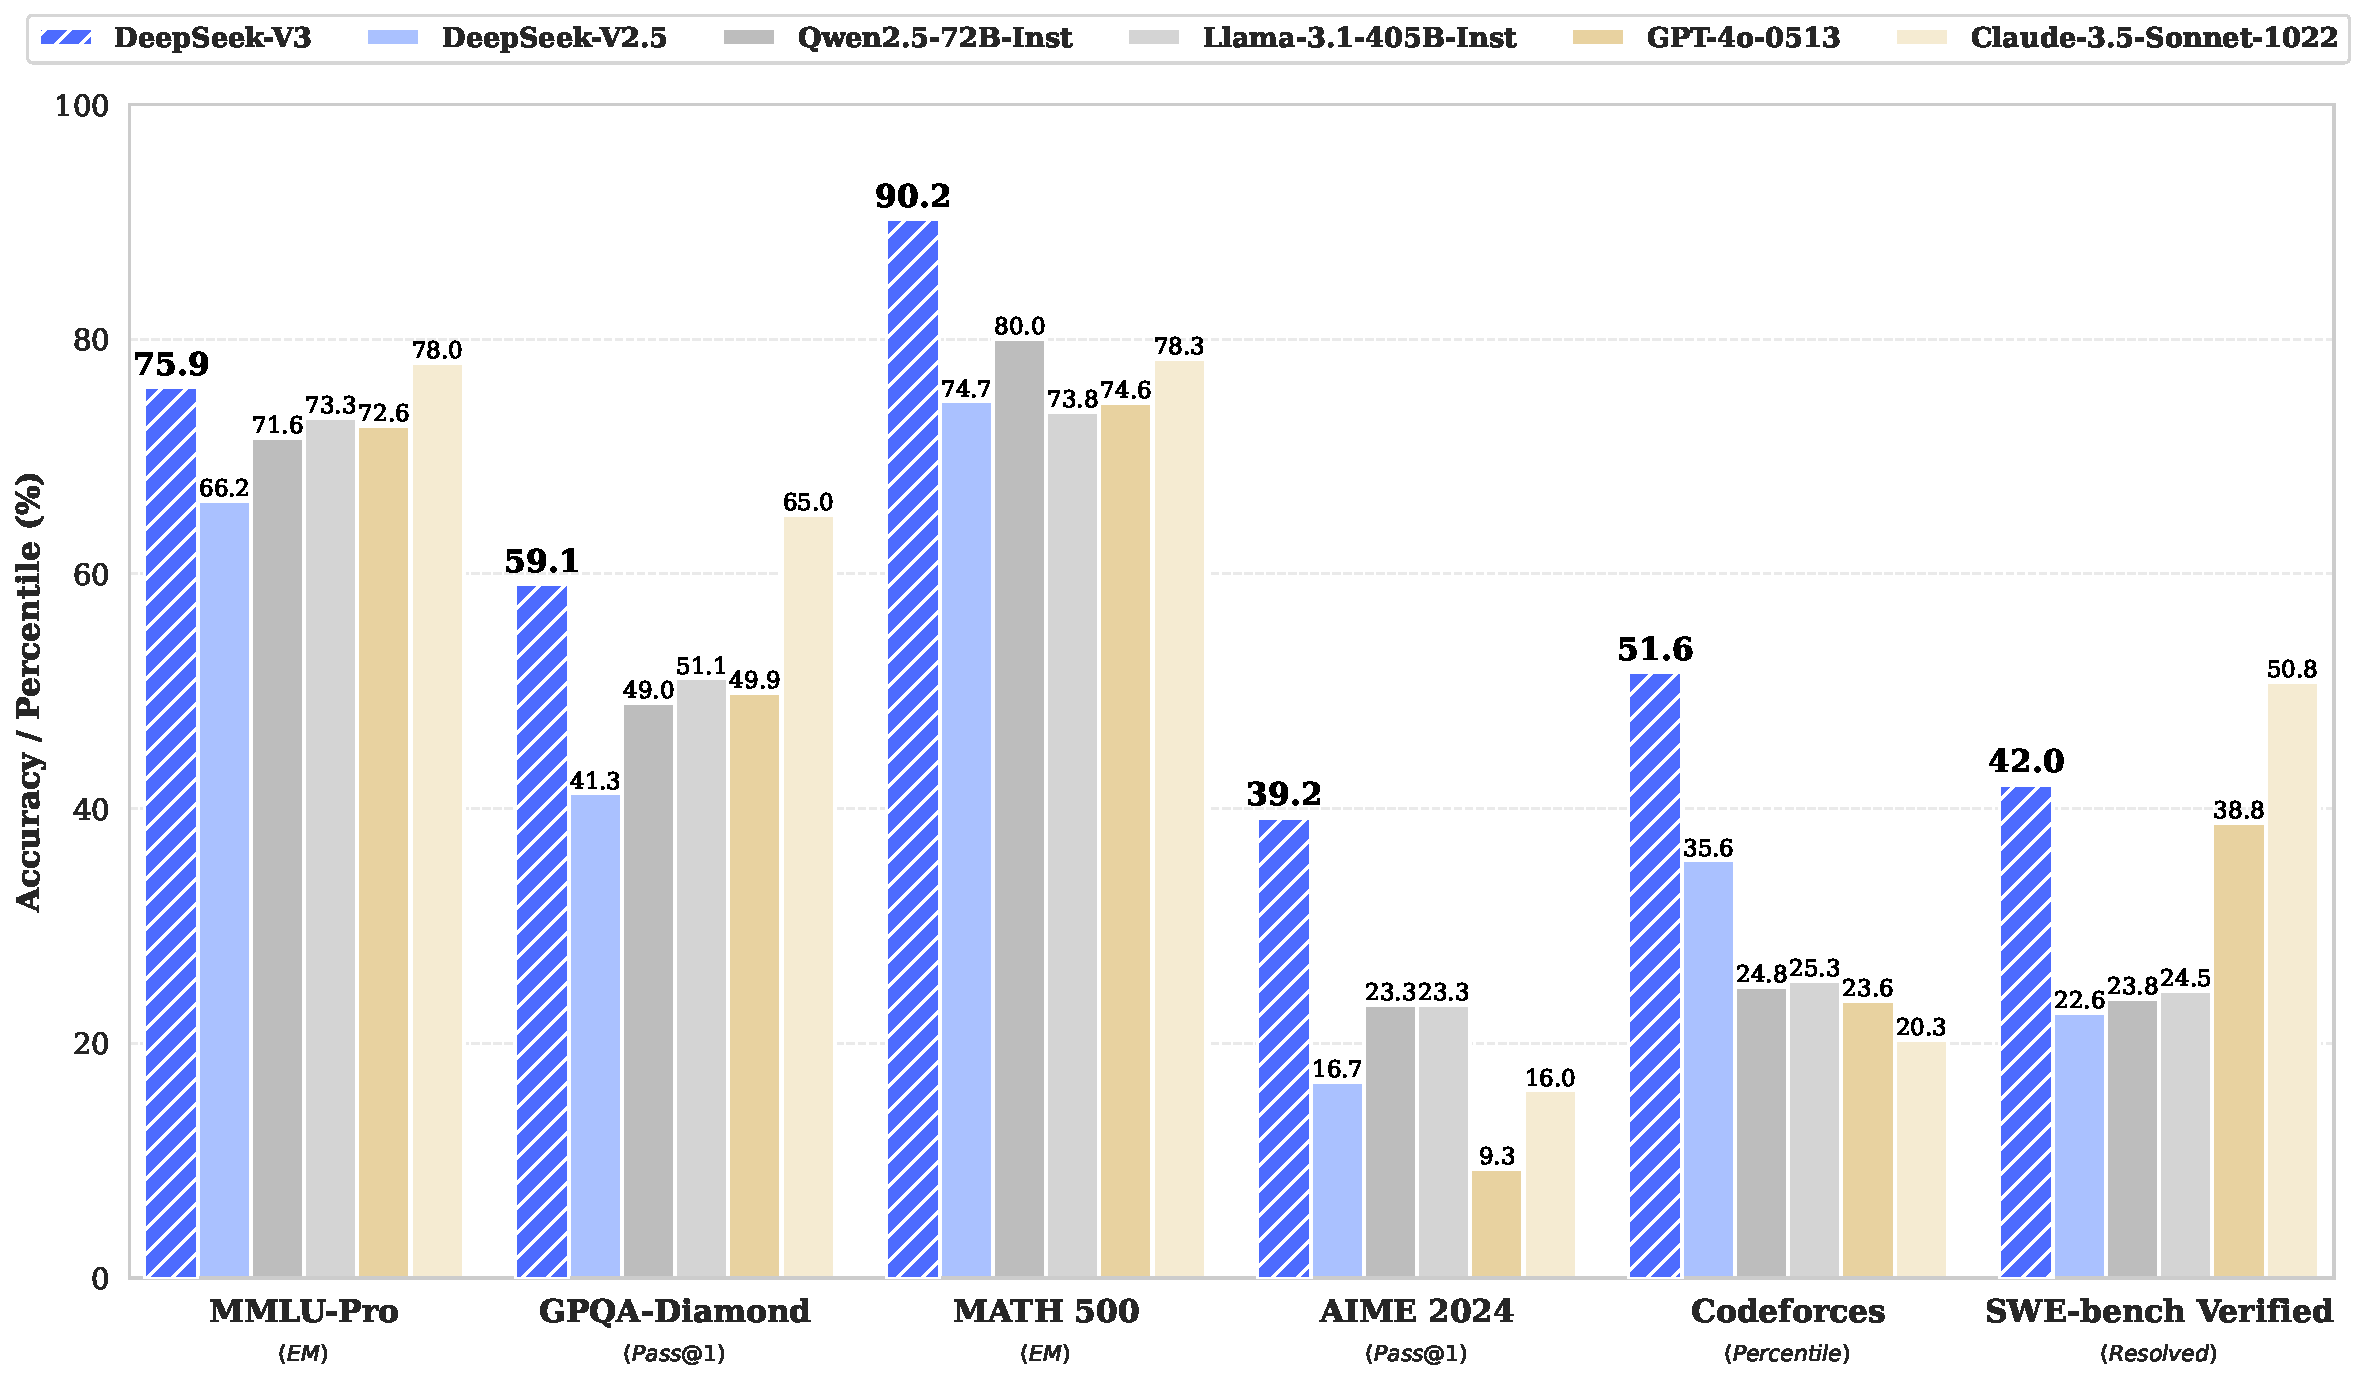
\includegraphics[width=\textwidth]{figures/dsv3_performance.pdf}
\caption{
    \centering
    \dsviii{} 和竞品在性能基准测试中的比较。
}
\label{fig:dsv3_performance}
\end{figure}

\newpage
\tableofcontents
\newpage

\section{简介}

近年来,大语言模型(Large Language Models, LLMs)正在经历快速的迭代和进化,逐步缩小与通用人工智能(Artificial General Intelligence, AGI)的差距。除了闭源模型外,开源模型,包括DeepSeek系列、LLaMA系列、Qwen系列和Mistral系列,也在取得显著进展,努力缩小与闭源模型的差距。为了进一步突破开源模型的能力边界,我们继续扩大模型规模,并推出了\dsviii{},这是一个拥有6710亿参数的大型混合专家(Mixture-of-Experts, MoE)模型,其中每个Token激活的参数量为370亿。

本着以终为始的精神,我们始终致力于实现强大的模型性能同时尽可能的节省训练和推理的成本。因此,在架构方面,\dsviii{}仍然采用多头潜在注意力(\dsattn{})以实现高效推理,以及采用\dsmoe{}以实现低成本的训练。这两种架构在\dsvii{}中得到了验证,证明了它们在保持模型强大性能的同时仍能实现高效的训练和推理。除了基础架构外,我们还实现了两种额外策略以进一步增强模型能力。首先,\dsviii{}首创了一种无辅助损失的负载均衡策略,旨在最小化负载均衡策略\footnote{因为负载均衡策略的使用不可避免}带来的模型性能下降。其次,\dsviii{}将多Token预测设定为训练目标。我们观察到,在评估基准上,整体性能提升了。

为了实现高效的训练,我们实现了FP8混合精度训练,并对训练框架进行了全面优化。低精度训练作为高效训练模型的一种解决方案,很有前景。其发展与硬件能力的进步密切相关。在本文所描述的工作中,我们引入了FP8混合精度训练框架,并首次在超大规模模型上验证了低精度训练的有效性。通过支持FP8的计算和存储,我们实现了训练的加速并减少了GPU内存的使用量。在训练框架方面,我们设计了 DualPipe 算法以实现高效的流水线并行,DualPipe 算法减少了流水线气泡,并通过计算-通信重叠(computation-communication overlap)隐藏了训练过程中的大部分通信。这种重叠确保了随着模型的进一步扩展,只要我们保持恒定的计算-通信比,就仍然可以在节点间使用细粒度的专家,同时实现近乎零的 All-to-All 通信开销。此外,我们还开发了高效的跨节点 All-to-All 通信内核,以充分利用InfiniBand和NVLink的带宽。此外,我们精心优化了内存占用,使得在不使用昂贵的张量并行的情况下,也能训练出\dsviii{}。通过这些努力,我们实现了高效的训练。

在预训练阶段,我们在14.8万亿个高质量且多样化的Token上训练出了\dsviii{}。预训练过程非常稳定。在整个训练过程中,我们没有遇到任何不可恢复的损失突增,也没有执行任何回滚操作。接下来,我们对\dsviii{}进行了两阶段的上下文长度扩展。在第一阶段,最大上下文长度扩展到32K,在第二阶段进一步扩展到128K。随后,我们对\dsviii{}的基础模型进行了后训练,包括监督微调(Supervised Fine-Tuning, SFT)和强化学习(Reinforcement Learning, RL),以使模型与人类偏好对齐并进一步释放模型的潜力。在后训练阶段,我们从DeepSeek-R1系列模型中蒸馏了推理能力,同时保持了模型准确性和生成长度之间的平衡。

我们在广泛的基准测试上对\dsviii{}进行了评估。尽管训练成本很低,综合评估表明,\dsviii{}-Base已成为当前最强的开源基础模型,尤其是在编程和数学领域。其聊天版本也在标准基准和开放式基准测试中优于其它开源模型,并与领先的闭源模型(包括GPT-4o和Claude-3.5-Sonnet)性能相当。

\begin{table}[t]
    \centering
    \setlength{\tabcolsep}{6pt}
    \begin{tabular}{l | c c c | c}
        \toprule
        \textbf{Training Costs} & \textbf{Pre-Training} & \textbf{Context Extension} & \textbf{Post-Training} & \textbf{Total} \\
        \midrule
        in H800 GPU Hours & 2664K & 119K & 5K & 2788K \\
        in USD & \$5.328M & \$0.238M & \$0.01M & \$5.576M \\
        \bottomrule
    \end{tabular}
    \caption{
    \dsviii{} 的训练花费,假设 H800 每个 GPU 小时的租赁费用是 \$2。
    }
    \label{tab:cost}
\end{table}

最后,我们再次强调\dsviii{}的训练成本非常低,具体见表~\ref{tab:cost}。这是通过我们对算法、框架和硬件的协同优化实现的。在预训练阶段,每万亿Token的训练仅需18万H800 GPU小时,也就是在我们自己的一个由 2048 个 H800 GPU 组成的集群上训练时间仅需 3.7 天。因此,我们花了不到两个月的时间就完成了模型的预训练,并只消耗了266.4万个GPU小时。结合上下文长度扩展所需的11.9万GPU小时和后训练所需的0.5万GPU小时,\dsviii{}的完整训练仅需278.8万GPU小时。假设H800 GPU的租赁价格为每小时2美元,我们的总训练成本仅为557.6万美元。需要注意的是,上述成本仅包括\dsviii{}的官方训练成本,不包括在架构、算法或数据上的前期研究和消融实验的相关成本。

我们的主要贡献包括:

\noindent
\textbf{架构:创新的负载均衡策略和训练目标}
\begin{itemize}[topsep=0pt]
    \item
    基于\dsvii{}使用的高效架构,我们首创了一种无辅助损失的负载均衡策略,最大限度地减少了因采用负载均衡而导致的性能下降。
    \item
    我们将多Token预测(Multi-Token Prediction, MTP)设置为训练目标,并证明其对模型性能有益。它还可以用于推测解码(speculative decoding)以实现推理加速。
\end{itemize}

\noindent
\textbf{预训练:向着终极的训练效率进发!}
\begin{itemize}[topsep=0pt]
    \item
    我们设计了一个FP8混合精度训练框架,并首次在超大规模模型上验证了FP8低精度训练的可行性和有效性。
    \item 
    通过算法、框架和硬件的协同设计,我们克服了跨节点MoE训练中的通信瓶颈,实现了近乎完全的计算-通信重叠。这显著提高了我们的训练效率并降低了训练成本,使我们能够在不增加额外开销的情况下进一步扩大模型规模。
    \item
    仅以266.4万个 H800 GPU 小时的成本,我们在14.8万亿Token上预训练出了DeepSeek-V3,它可以说是当前最强的开源基础模型。预训练后的后续训练阶段仅需10万GPU小时。
\end{itemize}

\noindent
\textbf{后训练:从DeepSeek-R1进行知识蒸馏}
\begin{itemize}[topsep=0pt]
    \item 
    我们引入了一种创新的方法,可以将长思维链(Chain-of-Thought, CoT)模型(特别是DeepSeek R1系列模型之一)的推理能力蒸馏到标准大语言模型(尤其是DeepSeek-V3)中。我们的工作巧妙地将R1的验证和反思能力融入了 DeepSeek-V3 模型中,显著提升了模型的推理性能。同时,我们还控制了DeepSeek-V3的输出风格和输出长度。
\end{itemize}

\noindent
\textbf{评估结果总结}
\begin{itemize}[topsep=0pt]
    \item \textbf{知识}:
    (1) 在教育类基准测试(如MMLU、MMLU-Pro和GPQA)上,DeepSeek-V3优于所有其它开源模型,在MMLU上得分为88.5,在MMLU-Pro上得分为75.9,在GPQA上得分为59.1。其性能与领先的闭源模型(如GPT-4o和Claude-Sonnet-3.5)相当,缩小了开源模型与闭源模型在该领域的差距。(2) 在事实性基准测试中,DeepSeek-V3在SimpleQA和中文SimpleQA上均表现出优于其他开源模型的性能。尽管在英文事实知识(SimpleQA)上略逊于GPT-4o和Claude-Sonnet-3.5,但在中文事实知识(中文SimpleQA)上超越了这些模型,凸显了其在中文事实知识方面的优势。
    \item \textbf{编程、数学和推理}: 
    (1) DeepSeek-V3在所有没有长思维链(CoT)的开源模型和闭源模型中,在数学相关基准测试上实现了最先进的性能。值得注意的是,它在特定基准测试(如MATH-500)上甚至优于o1-preview,展示了其强大的数学推理能力。(2) 在编程相关任务中,DeepSeek-V3成为编程竞赛基准测试(如LiveCodeBench)中表现最佳的模型,巩固了其在该领域的领先地位。在工程相关任务中,尽管DeepSeek-V3的表现略低于Claude-Sonnet-3.5,但它仍然显著领先于所有其它模型,展示了其在多样化技术基准测试中的竞争力。
\end{itemize}

在本文的剩余部分,我们首先详细阐述了\dsviii{}的模型架构(第\ref{sec:arch}节)。随后,介绍了基础设施,包括计算集群、训练框架、对FP8训练的支持、推理部署策略以及对未来AI硬件的一些设计建议。接下来,我们描述了预训练过程,包括训练数据的构建、超参数设置、长上下文扩展技术、相关评估以及一些讨论(第\ref{sec:pre-training}节)。之后,我们讨论了后训练过程,包括监督微调(SFT)、强化学习(RL)、相关评估和讨论(第\ref{sec:alignment}节)。最后,总结了这项工作,讨论了\dsviii{}的现有局限性,并提出了未来研究的潜在方向(第\ref{sec:conclusion}节)。

\section{架构}
\label{sec:arch}

首先来介绍 \dsviii{} 的基本架构。\dsviii{} 的特点是采用多头潜在注意力机制(Multi-head Latent Attention,\dsattn{})以实现高效推理,采用 \dsmoe{} 以实现模型的低成本训练。随后,我们提出了将多Token预测(Multi-Token Prediction,MTP)设定为训练目标的方案,并观察到它能够提升评估基准上的整体性能。对于其它没有明确提及的小细节,\dsviii{} 沿用了 \dsvii{} 的设置。

\begin{figure}[!t]
\centering
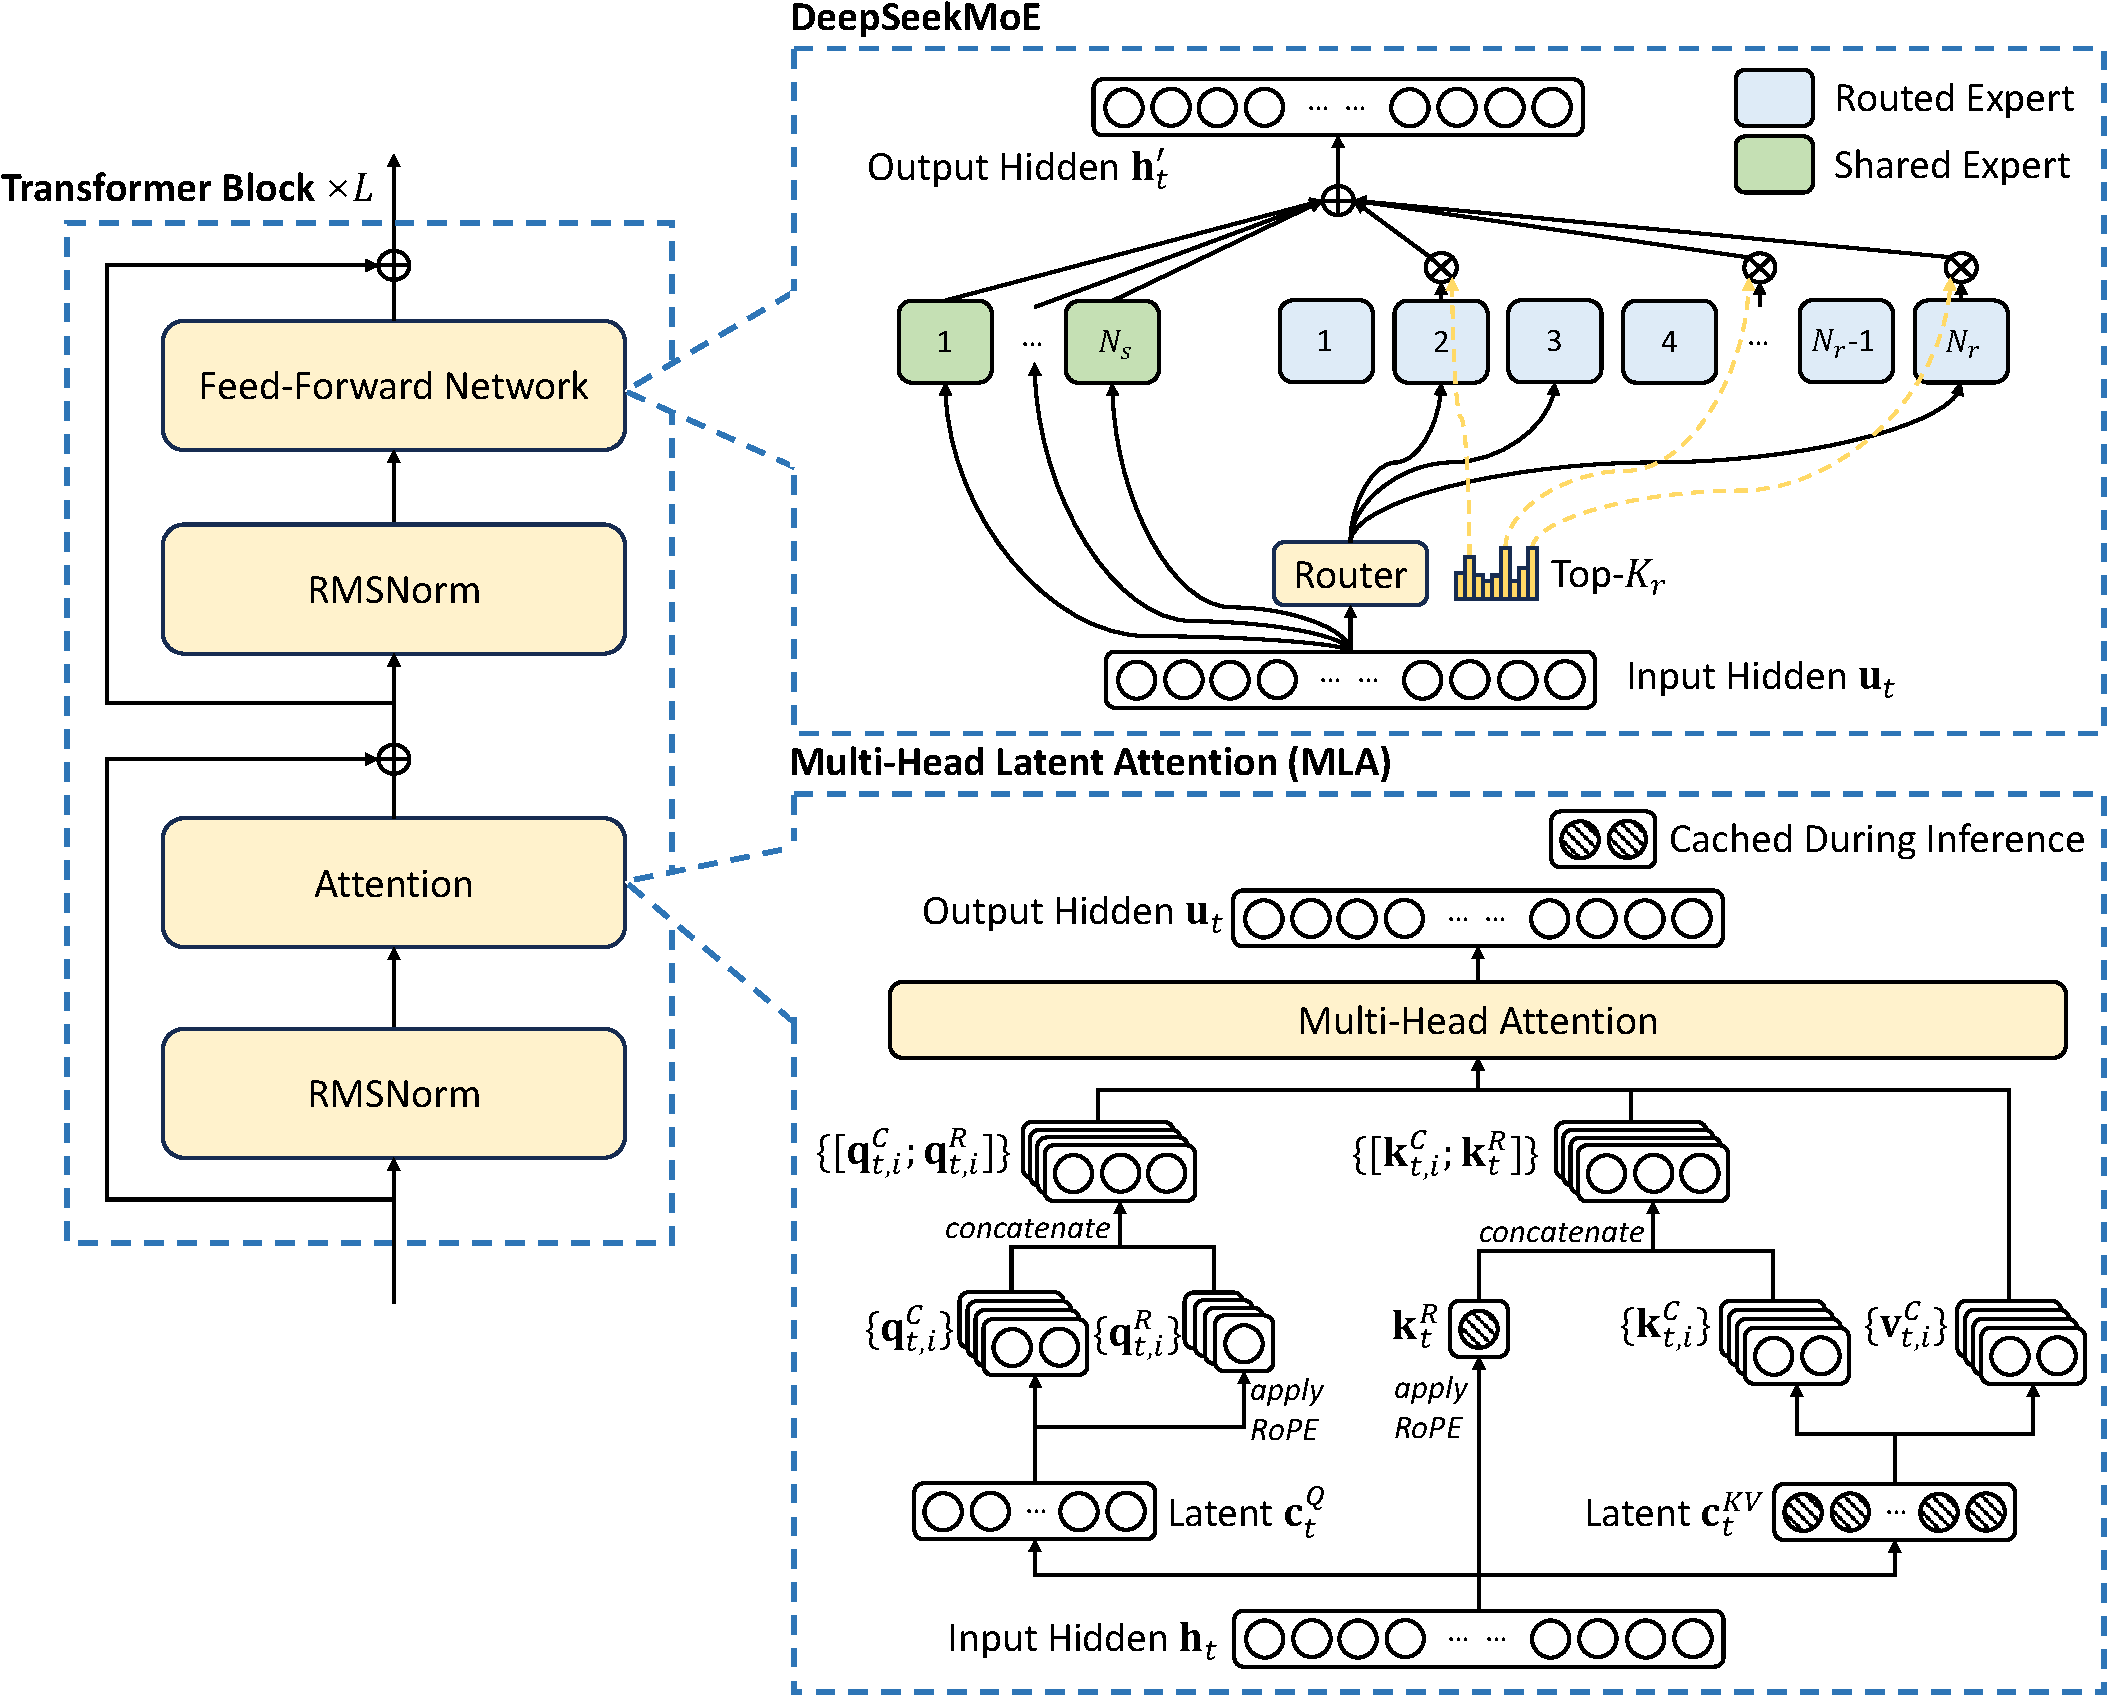
\includegraphics[width=0.99\linewidth]{figures/basic_arch.pdf}
\caption{
    \dsviii{} 的基本架构图,\dsviii{} 延续了 \dsvii{} 的思想,采用了 \dsattn{} 和 \dsmoe{} 来实现高效的推理和低成本的训练。
}
\label{fig:basic_arch}
\end{figure}

\subsection{基本架构}

\dsviii{} 的基本架构仍然没有脱离 Transformer 。为了实现高效的推理和低成本的训练,\dsviii{} 还采用了 \dsattn{} 和 \dsmoe{},这两者已在 \dsvii{} 中得到了充分验证。与 \dsvii{} 相比,\dsviii{} 有一点不同,那就是我们额外引入了一种无辅助损失的负载均衡策略,从而减轻了采用负载平衡策略所带来的性能下降。图~\ref{fig:basic_arch} 展示了 \dsviii{} 的基本架构,我们将在本节中简要回顾 MLA 和 DeepSeekMoE 的细节。

\subsubsection{多头潜在注意力机制(Multi-Head Latent Attention)}

在注意力机制方面,\dsviii{} 采用了 \dsattn{} 架构。设 $d$ 表示嵌入的维度,$n_h$ 表示注意力头的数量,$d_h$ 表示每个头的维度,$\mathbf{h}_{t} \in \mathbb{R}^{d}$ 表示在给定的注意力层中第 $t$ 个 Token 的注意力输入。\dsattn{} 的核心是对注意力的键(keys)和值(values)进行低秩(low-rank)联合压缩,以减少推理过程中键-值(Key-Value,KV)缓存的使用:

\begin{align}
    \boxed{\color{blue} \mathbf{c}_{t}^{KV}} &= W^{DKV} \mathbf{h}_{t}, \\
    [\mathbf{k}_{t, 1}^{C};\mathbf{k}_{t, 2}^{C};...;\mathbf{k}_{t, n_{h}}^{C}] = \mathbf{k}_{t}^{C} &= W^{UK} \mathbf{c}_{t}^{KV}, \\
    \boxed{\color{blue}\mathbf{k}_{t}^{R}} &= \operatorname{RoPE}({W^{KR}} \mathbf{h}_{t}), \\
    \mathbf{k}_{t, i} &= [\mathbf{k}_{t, i}^{C}; \mathbf{k}_{t}^{R}], \\
    [\mathbf{v}_{t, 1}^{C};\mathbf{v}_{t, 2}^{C};...;\mathbf{v}_{t, n_{h}}^{C}] = \mathbf{v}_{t}^{C} &= W^{UV} \mathbf{c}_{t}^{KV}, 
\end{align}

其中 $\mathbf{c}_{t}^{KV} \in \mathbb{R}^{d_c}$ 是键和值的压缩潜在向量;$d_c (\ll d_h n_h)$ 表示 KV 的压缩维度;$W^{DKV} \in \mathbb{R}^{d_c \times d}$ 表示下投影矩阵(down-projection matrix);$W^{UK}, W^{UV} \in \mathbb{R}^{d_h n_h \times d_c}$ 表示键和值的上投影矩阵(up-projection matrix);$W^{KR} \in \mathbb{R}^{d_h^R \times d}$ 是用于生成解耦键(decoupled key)的矩阵,解耦键携带了旋转位置嵌入(Rotary Positional Embedding,RoPE);$\operatorname{RoPE}(\cdot)$ 表示应用 RoPE 矩阵的运算;$[\cdot;\cdot]$ 表示拼接。请注意,对于 MLA,只有蓝框中的向量(即 $\color{blue} \mathbf{c}_{t}^{KV}$ 和 $\color{blue}\mathbf{k}_{t}^{R}$)需要在生成过程中缓存,而这可以显著减少 KV 缓存,同时保持与标准多头注意力(Multi-Head Attention,MHA)相当的性能。

对于注意力查询(queries),我们也进行了低秩压缩,这可以减少训练过程中的激活内存:

\begin{align}
    \mathbf{c}_{t}^{Q} &= W^{DQ} \mathbf{h}_{t}, \\
    [\mathbf{q}_{t, 1}^{C};\mathbf{q}_{t, 2}^{C};...;\mathbf{q}_{t, n_{h}}^{C}] = \mathbf{q}_{t}^{C} &= W^{UQ} \mathbf{c}_{t}^{Q}, \\
    [\mathbf{q}_{t, 1}^{R};\mathbf{q}_{t, 2}^{R};...;\mathbf{q}_{t, n_{h}}^{R}] = \mathbf{q}_{t}^{R} &= \operatorname{RoPE}({W^{QR}} \mathbf{c}_{t}^{Q}), \\
    \mathbf{q}_{t, i} &= [\mathbf{q}_{t, i}^{C}; \mathbf{q}_{t, i}^{R}],
\end{align}

其中 $\mathbf{c}_{t}^{Q} \in \mathbb{R}^{d_c^{\prime}}$ 是查询(queries)的压缩潜在向量;$d_c^{\prime} (\ll d_h n_h)$ 表示查询压缩维度;$W^{DQ} \in \mathbb{R}^{d_c^{\prime} \times d}, W^{UQ} \in \mathbb{R}^{d_h n_h \times d_c^{\prime}}$ 分别是查询的下投影矩阵和上投影矩阵;$W^{QR} \in \mathbb{R}^{d_h^R n_h \times d_c^{\prime}}$ 是一个矩阵,用来生成携带 RoPE 的解耦查询。

最终,通过组合注意力查询 ($\mathbf{q}_{t, i}$)、键 ($\mathbf{k}_{j, i}$) 和值 ($\mathbf{v}_{j, i}^{C}$) 来产生最终的注意力输出 $\mathbf{u}_{t}$:

\begin{align}
    \mathbf{o}_{t, i} &= \sum_{j=1}^{t} \operatorname{Softmax}_j(\frac{\mathbf{q}_{t, i}^T \mathbf{k}_{j, i}}{\sqrt{d_{h} + d_{h}^{R}}}) \mathbf{v}_{j, i}^{C}, \\
    \mathbf{u}_{t} &= W^{O} [\mathbf{o}_{t, 1};\mathbf{o}_{t, 2};...;\mathbf{o}_{t, n_{h}}],
\end{align}

其中 $W^{O} \in \mathbb{R}^{d \times d_h n_h}$ 表示输出投影矩阵(projection matrix)。

\subsubsection{带有无辅助损失负载均衡的\dsmoe{}}

\paragraph{\dsmoe{} 的基本架构。}
对于前馈网络(Feed-Forward-Networks),\dsviii{} 采用了 \dsmoe{} 架构。与传统的 MoE 架构(如 GShard)相比,\dsmoe{} 使用了更细粒度的专家,并将一些专家隔离作为共享专家。设 $\mathbf{u}_{t}$ 表示第 $t$ 个 Token 的前馈网络输入,并计算前馈网络的输出 $\mathbf{h}_{t}^{\prime}$ 如下:

\begin{align}
    \mathbf{h}_{t}^{\prime} & = \mathbf{u}_{t} + \sum_{i=1}^{N_{s}} {\operatorname{FFN}^{(s)}_{i}\left( \mathbf{u}_{t} \right)} + \sum_{i=1}^{N_r} {g_{i,t} \operatorname{FFN}^{(r)}_{i}\left( \mathbf{u}_{t} \right)}, \\
    g_{i,t} & = \frac{g^{\prime}_{i,t}}{\sum_{j=1}^{N_r} g^{\prime}_{j,t}}, \\
    g^{\prime}_{i,t} & = \begin{cases} 
    s_{i,t}, & s_{i,t} \in \operatorname{Topk} (\{ s_{j, t} | 1 \leq j \leq N_r \}, K_{r}), \\
    0, & \text{otherwise}, 
    \end{cases} \\
    s_{i,t} & = \operatorname{Sigmoid} \left( {\mathbf{u}_{t}}^{T} \mathbf{e}_{i} \right),
\end{align}

其中 $N_{s}$ 和 $N_r$ 分别表示共享专家的数量和路由专家的数量; $\operatorname{FFN}^{(s)}_{i}(\cdot)$ 和 $\operatorname{FFN}^{(r)}_{i}(\cdot)$ 分别表示第 $i$ 个共享专家和第 $i$ 个路由专家; $K_{r}$ 表示激活的路由专家数量; $g_{i,t}$ 是第 $i$ 个专家的门控值; $s_{i,t}$ 是 Token 与专家的亲和度; $\mathbf{e}_{i}$ 是第 $i$ 个路由专家的中心向量; $\operatorname{Topk}(\cdot, K)$ 表示包含 $K$ 个最高分数的集合,这些分数是为第 $t$ 个 Token 和所有路由专家计算的亲和度分数。与 \dsvii{} 略有不同,\dsviii{} 使用 Sigmoid 函数来计算亲和度分数,并对所有选定的亲和度分数进行归一化,从而生成门控值。

\paragraph{无辅助损失的负载均衡。}
对于 MoE 模型,不均衡的专家负载会导致路由崩溃,并在专家并行的场景中降低计算效率。传统的解决方案通常依赖于辅助损失来避免负载不均衡。然而,过大的辅助损失会损害模型性能。为了在负载均衡和模型性能之间实现更好的权衡,我们首创了一种无辅助损失的负载均衡策略,以确保负载均衡。

具体来说,我们为每个专家引入一个偏置项 $b_i$,并将其添加到相应的亲和度分数 $s_{i,t}$ 中,以确定 top-K 路由:

\begin{align}
    g^{\prime}_{i,t} & = \begin{cases} 
    s_{i,t}, & s_{i,t} + b_i \in \operatorname{Topk} (\{ s_{j, t} + b_j | 1 \leq j \leq N_r \}, K_{r}), \\
    0, & \text{otherwise}.
    \end{cases}
\end{align}

请注意,偏置项仅用于路由。门控值将与前馈网络的输出相乘,且门控值仍然来源于原始的亲和度分数 $s_{i,t}$。在训练过程中,我们会持续监控每个训练步骤中整个批次(batch)的专家负载。在每个步骤结束时,如果有某个专家负载过高,我们会将这个专家对应的偏置项减少 $\gamma$;如果某个专家负载不足,则增加相应的 $\gamma$,其中 $\gamma$ 是一个称为偏置更新速度的超参数。通过动态调整,\dsviii{} 在训练过程中维持了专家的负载均衡,并且实现了比那些采用了纯辅助损失负载均衡策略的模型更好的性能。

\paragraph{互补的序列级辅助损失。}
虽然 \dsviii{} 主要依赖于无辅助损失的负载均衡策略,但为了防止单个序列内部的负载极端不均衡,我们还采用了互补的序列级均衡损失:

\begin{align}
    \mathcal{L}_{\mathrm{Bal}} & = \alpha \sum_{i=1}^{N_r}{f_i P_i}, \\
    % f_i = \frac{N_r}{K_r T} \sum_{t=1}^{T} \mathds{1}( \text{Expert $i$ } & \text{belongs to the Top-$K_r$ set for Token $t$} ), \\
    f_i = \frac{N_r}{K_r T} \sum_{t=1}^{T} \mathds{1} & \left( s_{i,t} \in \operatorname{Topk} ( \{ s_{j, t} | 1 \leq j \leq N_r \}, K_{r} ) \right), \\
    s^{\prime}_{i,t} & = \frac{s_{i,t}}{\sum_{j=1}^{N_r} s_{j,t}}, \\
    P_i & = \frac{1}{T} \sum_{t=1}^{T}{s^{\prime}_{i,t}},
\end{align}

其中均衡因子 $\alpha$ 是一个超参数,针对 \dsviii{} 会被赋予一个极小的值;$\mathds{1}(\cdot)$ 表示指示函数;$T$ 表示序列中 Token 的数量。序列级均衡损失会尽量使得每个序列的专家负载保持均衡。

\paragraph{限制节点数量的路由。}
与 \dsvii{} 使用的设备限制路由类似,\dsviii{} 也采用了一种受限路由机制,以限制训练过程中的通信成本。简而言之,我们确保每个 Token 最多只会被发送到 $M$ 个节点,这些节点是根据分布在每个节点上的专家的最高 $\frac{K_r}{M}$ 个亲和度分数之和进行选择的。在这个约束下,我们的 MoE 训练框架几乎可以实现完全的计算-通信重叠。

\paragraph{不丢弃任何Token}
由于采用了有效的负载均衡策略,\dsviii{} 在整个训练过程中都保持了良好的负载均衡。因此,\dsviii{} 在训练过程中不会丢弃任何 Token。此外,我们还实现了特定的部署策略,以确保推理的负载均衡,因此 \dsviii{} 在推理过程中也不会丢弃任何 Token。

\begin{figure}[!t]
\centering
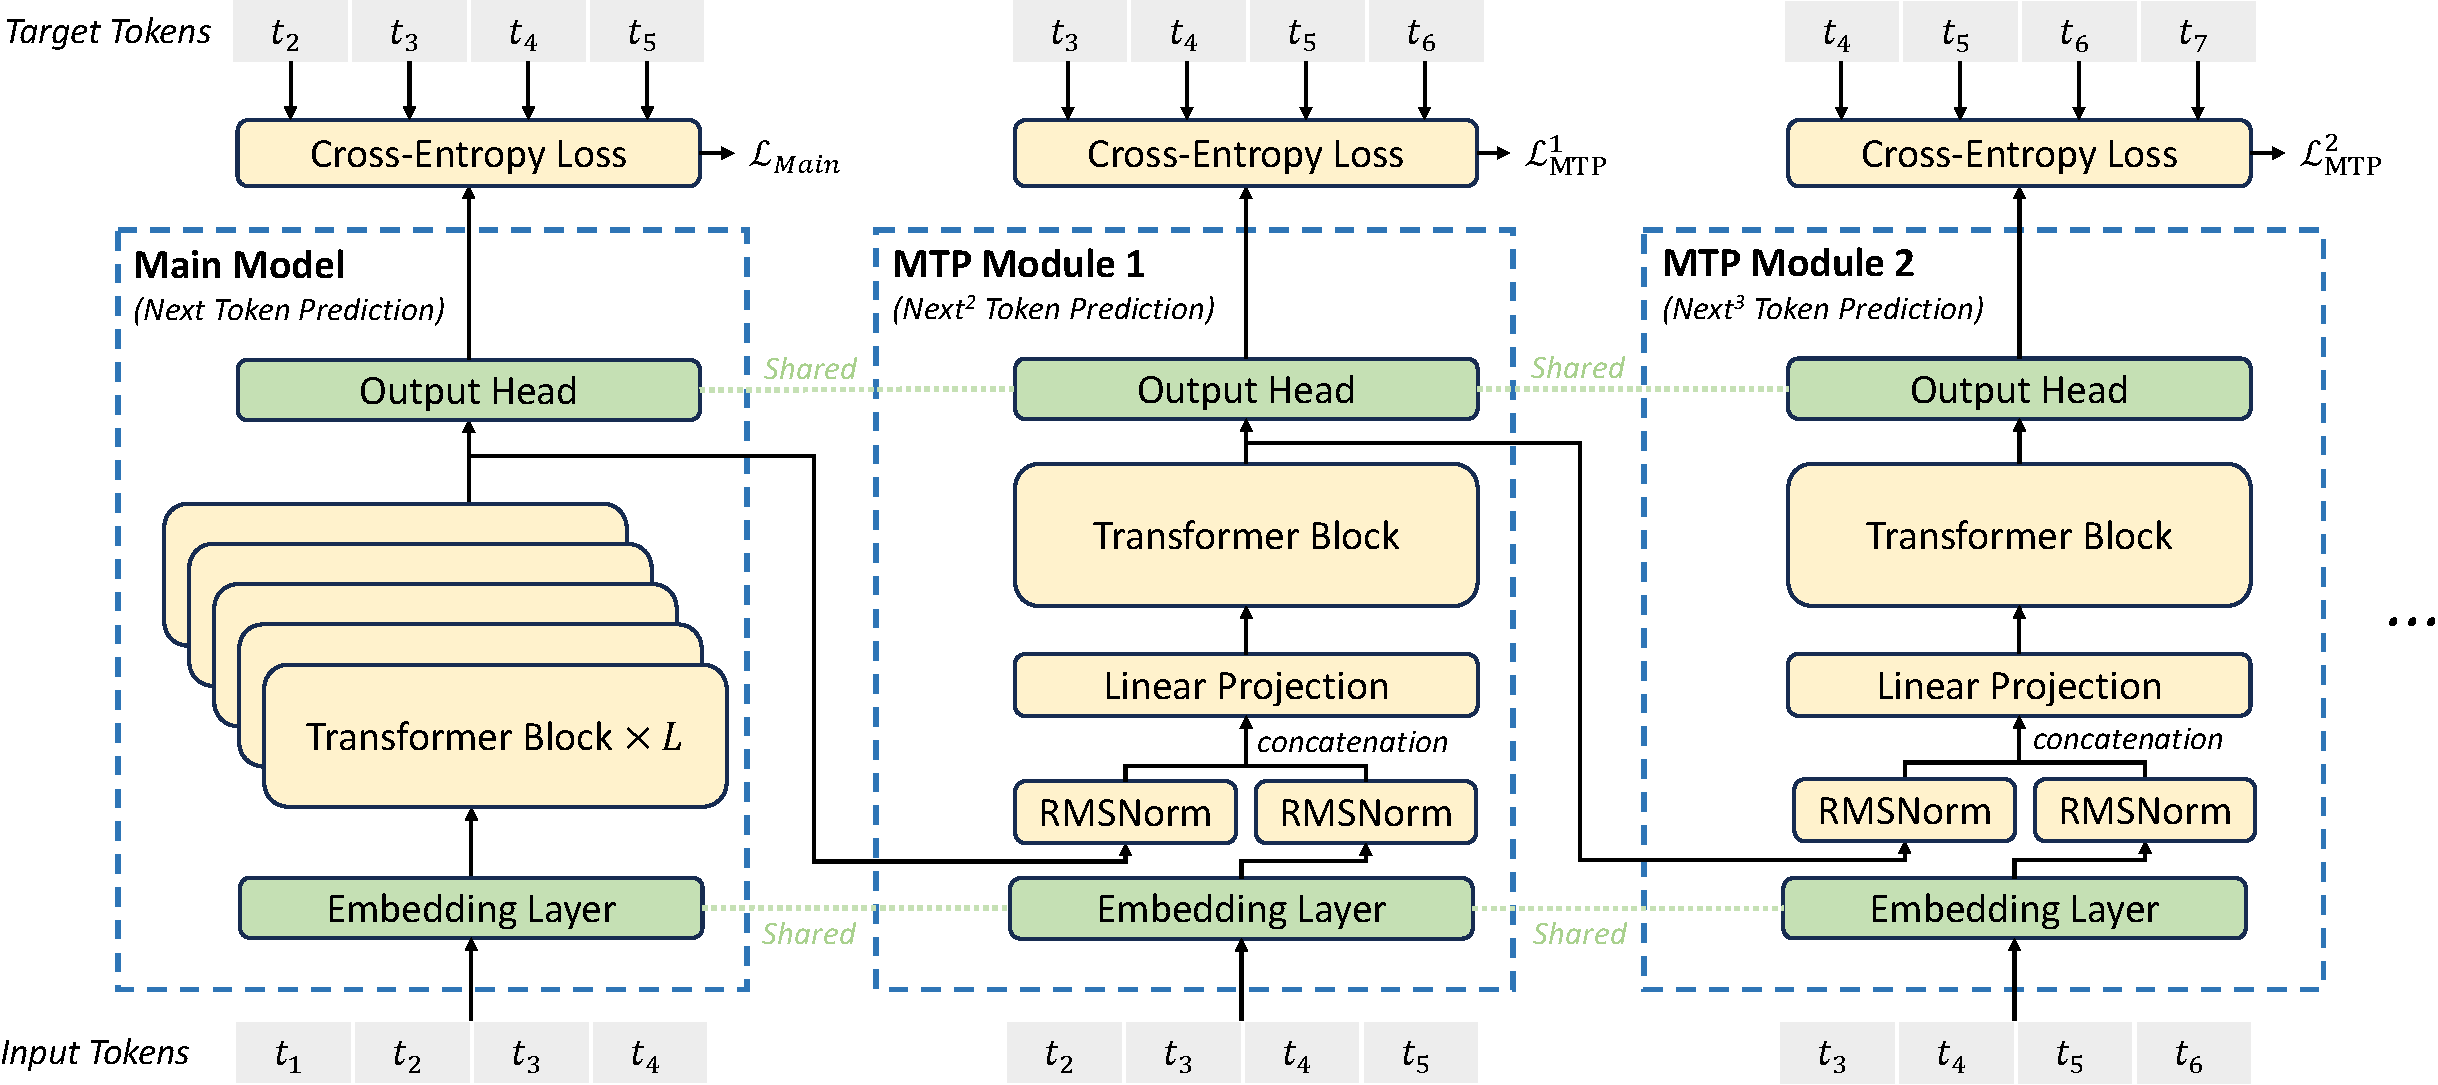
\includegraphics[width=0.99\linewidth]{figures/nextn.pdf}
\caption{多Token预测的实现架构图。针对每个深度的每个Token的预测,我们都会维护完整的因果链。}
\label{fig:nextn}
\end{figure}

\subsection{多Token预测(Multi-Token Prediction)}

受到文章《Better \& faster large language models via multi-token prediction》的启发,我们为 \dsviii{} 研究并设定了多 Token 预测(MTP)训练目标。这样训练目标就将预测范围扩展到每个位置的多个未来Token。一方面,MTP 训练目标密集化了训练信号,有可能提高数据效率。另一方面,MTP 可能使模型能够提前规划其表示,以更好地预测未来的Token。图~\ref{fig:nextn} 展示了我们对 MTP 的实现。与《Better \& faster large language models via multi-token prediction》使用独立输出头来并行预测 $D$ 个额外 Token 不同,我们是顺序的预测了额外的Token,并在每个预测深度都维护了完整的因果链。在本节中,我们将介绍 MTP 实现的详细信息。

\paragraph{MTP模块。}
具体来说,我们的 MTP 实现使用 $D$ 个顺序模块来预测 $D$ 个额外的Token。第 $k$ 个 MTP 模块由一个共享的嵌入层 $\operatorname{Emb}(\cdot)$、一个共享的输出头 $\operatorname{OutHead}(\cdot)$、一个 Transformer 块 $\operatorname{TRM}_k(\cdot)$ 和一个投影矩阵 $M_k \in \mathbb{R}^{d \times 2d}$ 组成。对于第 $i$ 个输入的Token $t_i$,在第 $k$ 个预测深度,我们首先将第 $(k-1)$ 深度的第 $i$ 个 Token 的表示 $\mathbf{h}_i^{k-1} \in \mathbb{R}^{d}$ 与第 $(i+k)$ 个 Token 的嵌入 $Emb(t_{i+k}) \in \mathbb{R}^{d}$ 通过线性投影结合起来:

\begin{equation}
    \mathbf{h}_i^{\prime k} = M_k [\operatorname{RMSNorm}(\mathbf{h}_i^{k-1}) ; \operatorname{RMSNorm}(\operatorname{Emb}(t_{i+k}))],
\end{equation}

其中 $[\cdot ; \cdot]$ 表示拼接。特别地,当 $k=1$ 时,$\mathbf{h}_i^{k-1}$ 指的是主模型给出的表示。注意,对于每个 MTP 模块,它的嵌入层会和主模型共享。结合后的 $\mathbf{h}_i^{\prime k}$ 作为第 $k$ 个深度的 Transformer 块的输入,以生成当前深度的输出表示 $\mathbf{h}_{i}^{k}$:

\begin{equation}
    \mathbf{h}_{1:T-k}^{k} = \operatorname{TRM}_k(\mathbf{h}_{1:T-k}^{\prime k}),
\end{equation}

其中 $T$ 表示输入序列的长度,$_{i:j}$ 表示切片运算(包括左右边界)。最后,以 $\mathbf{h}_{i}^{k}$ 作为输入,共享的输出头将计算第 $k$ 个额外预测的 Token 的概率分布 $P_{i+1+k}^{k} \in \mathbb{R}^{V}$,其中 $V$ 是词汇表的大小:

\begin{equation}
    P_{i+k+1}^{k} = \operatorname{OutHead}(\mathbf{h}_{i}^{k}).
\end{equation}

输出头 $\operatorname{OutHead}(\cdot)$ 会将\underline{表示}线性映射成logits,随后使用 $\operatorname{Softmax}(\cdot)$ 函数来计算第 $k$ 个额外 Token 的预测概率。此外,对于每个 MTP 模块,其输出头也与主模型共享。我们维护预测的因果链的原则和EAGLE维护预测的因果链的原则是一样的,但EAGLE的主要目标是推测解码,而我们是利用 MTP 来改善训练。

\paragraph{MTP 训练目标。}
对于每个预测深度,我们计算交叉熵损失 $\mathcal{L}_{\text{MTP}}^{k}$:

\begin{equation}
    \mathcal{L}_{\text{MTP}}^{k} = \operatorname{CrossEntropy}(P_{2 + k:T + 1}^{k}, t_{2 + k:T + 1}) = -\frac{1}{T} \sum_{i=2 + k}^{T + 1} \log P_i^k [t_i],
\end{equation}

其中 $T$ 表示输入序列的长度,$t_i$ 表示第 $i$ 个位置的真实 Token,$P_i^k [t_i]$ 表示由第 $k$ 个 MTP 模块给出的 $t_i$ 的相应预测概率。最后,我们计算所有深度的 MTP 损失的平均值,并乘以一个权重因子 $\lambda$,以获得整体 MTP 损失 $\mathcal{L}_{\text{MTP}}$,作为 \dsviii{} 的额外训练目标:

\begin{equation}
    \mathcal{L}_{\text{MTP}} = \frac{\lambda}{D} \sum_{k=1}^{D} \mathcal{L}_{\text{MTP}}^{k}.
\end{equation}

\paragraph{推理中的 MTP。}
MTP策略旨在提高主模型的性能,因此在推理过程中,我们可以直接丢弃 MTP 模块,主模型也可以独立且正常地运行。此外,我们还可以将这些 MTP 模块重新用于推测解码,以进一步改进生成的延迟。

\section{基础设施}
\label{sec:infra}

\subsection{计算集群}

\dsviii{} 在一个配备 2048 个 NVIDIA H800 GPU 的集群上进行训练。每个 H800 集群节点包含 8 个通过 NVLink 和 NVSwitch 连接的 GPU。不同节点之间使用 InfiniBand 互连来促进通信。

\subsection{训练框架}

\dsviii{} 的训练得益于 HAI-LLM 框架,这是我们的工程师从零开始打造的高效轻量级训练框架。总体而言,\dsviii{} 使用了 16 路流水线并行(Pipeline Parallelism)、跨越 8 个节点的 64 路专家并行(Expert Parallelism)和 ZeRO-1 数据并行(Data Parallelism)。

为了促进 \dsviii{} 的高效训练,我们进行了细致的工程优化。首先,我们设计了 DualPipe 算法以实现高效的流水线并行。与现有的流水线并行方法相比,DualPipe 具有更少的流水线气泡。更重要的是,它在前向和反向过程中重叠计算和通信阶段,从而解决了跨节点专家并行带来的高通信开销问题。其次,我们开发了高效的跨节点All-to-All通信内核,以充分利用 InfiniBand 和 NVLink 带宽,从而将专用于通信的流式多处理器(SM)节省了一部分出来。最后,我们在训练过程中仔细优化了内存占用,从而使我们能够在不使用昂贵的张量并行(Tensor Parallelism)的情况下训练 \dsviii{}。

\subsubsection{DualPipe和计算-通信叠加}

\begin{figure}[t]
    \centering
    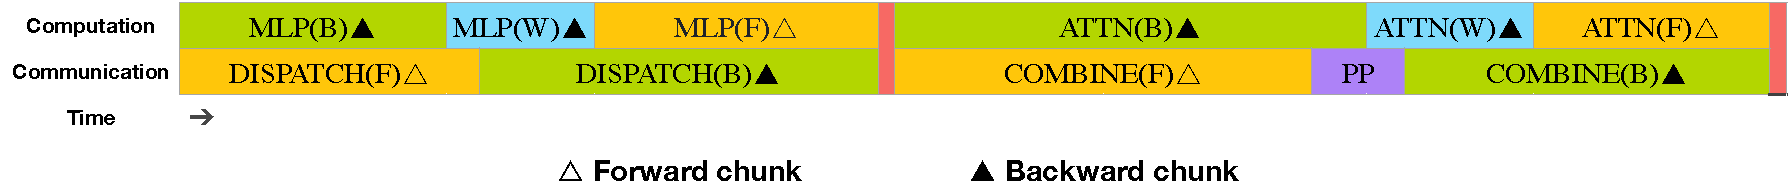
\includegraphics[width=0.9\textwidth]{figures/overlap.pdf}
    \caption{针对一对儿独立的前向和反向计算块的重叠策略(Transformer块的边界未对齐)。橙色表示前向,绿色表示“输入的反向”,蓝色表示“权重的反向”,紫色表示流水线并行通信,红色表示屏障。All-to-All通信和流水线并行通信都可以完全隐藏。
    }
    \label{fig:transformer-overlap}
\end{figure}

对于 \dsviii{},跨节点专家并行引入的通信开销导致计算-通信比约为 1:1,这使得效率低下。为了解决这一挑战,我们设计了一种创新的流水线并行算法,称为 DualPipe 算法,它不仅通过有效重叠前向和反向计算-通信阶段来加速模型训练,还减少了流水线气泡的产生。

DualPipe 算法的关键思想是在一对前向和反向块内重叠计算和通信。具体来说,我们将每个块分为四个组件:\texttt{attention}、\texttt{all-to-all dispatch}、\texttt{MLP} 和 \texttt{all-to-all combine}。特别地,对于反向块,\texttt{attention} 和 \texttt{MLP} 进一步拆分为两个部分:\texttt{输入的backward} 和 \texttt{权重的backward},类似于ZeroBubble。此外,我们还有一个 \texttt{流水线并行通信} 组件。如图~\ref{fig:transformer-overlap} 所示,对于一对前向和反向块,我们重新排列这些组件,并手动调整专用于通信与计算的 GPU 流式多处理器的比例。在这种重叠策略中,我们可以确保在执行期间,所有All-to-All通信和流水线并行通信可以完全隐藏。由于采用了高效的重叠策略,完整的 DualPipe 算法调度如图~\ref{fig:dualpipe-schedules} 所示。它采用双向管道调度,也就是同时从管道的两端输入微批次(micro batch),这样大量通信就可以完全重叠了。这种重叠还确保了,即使模型会进一步扩展,只要我们保持恒定的计算-通信比,就可以在节点之间使用细粒度的专家,同时将All-to-All通信的开销降低到接近于零。

\begin{figure}[t]
    \centering
    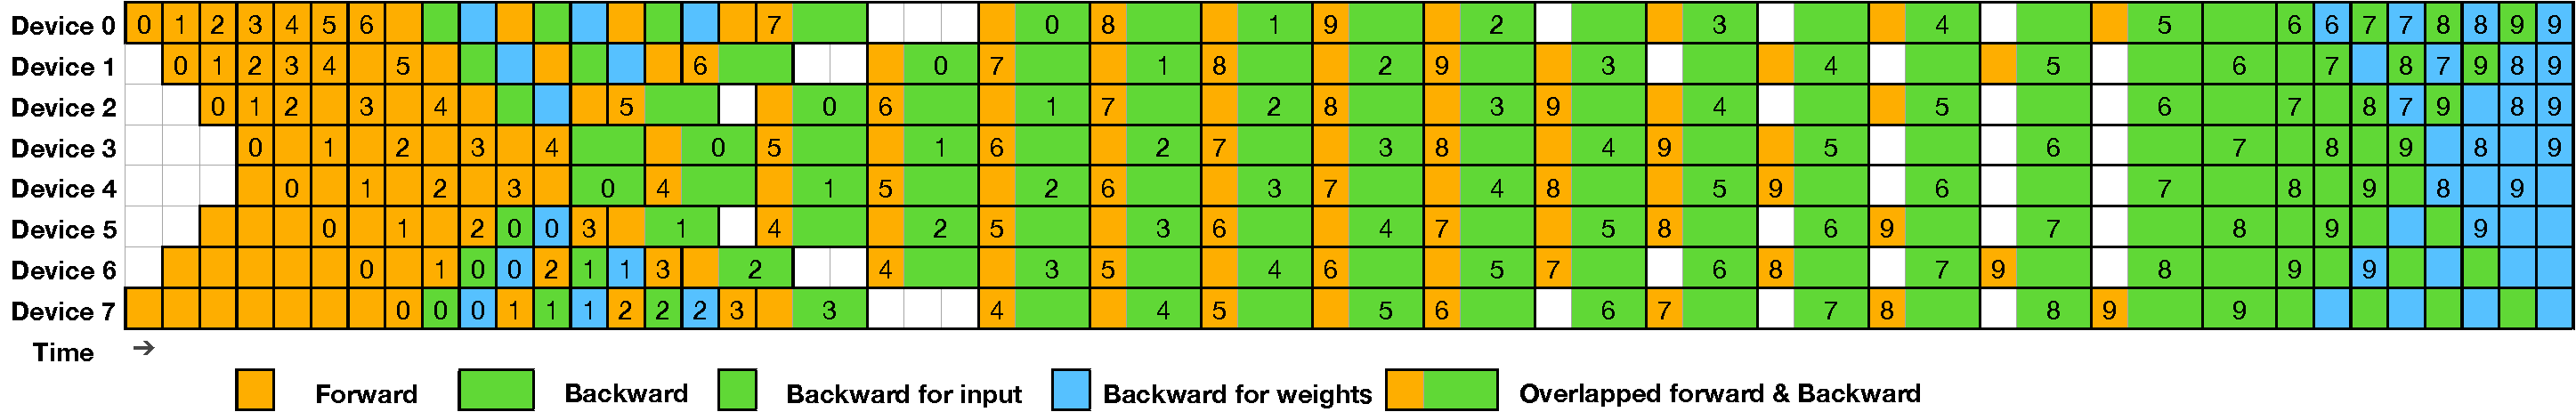
\includegraphics[width=0.99\linewidth]{figures/dualpipe.pdf}
    \caption{
        8个PP排名和20个微批次在两个方向上的DualPipe调度示例。反向方向上的微批次与前向方向上的微批次对称,因此为了简化说明,我们省略了它们的批次ID。两个由共享黑色边框围住的单元具有相互重叠的计算和通信。
    }
    \label{fig:dualpipe-schedules}
\end{figure}

此外,即使在通信开销不高的那些更一般的场景中,DualPipe 算法仍然表现出效率优势。在表~\ref{tab:dualpipe-bubble} 中,我们总结了不同的流水线并行方法的流水线气泡和内存使用情况。如表中所示,与 ZB1P 和 1F1B 相比,DualPipe 算法显著减少了流水线气泡,同时仅将峰值激活内存增加了 $\frac{1}{PP}$ 倍。尽管 DualPipe 算法需要维护两份模型参数的副本,但由于我们在训练中使用了较大的专家并行规模,所以这并不会显著增加内存消耗。与 Chimera 相比,DualPipe 算法仅要求管道的阶段数量和微批次数量可被 2 整除就行,而不要求微批次数量可被管道的阶段数量整除。此外,对于 DualPipe 算法,随着微批次数量的增加,流水线气泡和激活内存都不会增加。

\begin{table}[t]
    \centering
    \setlength{\tabcolsep}{15pt}
    \begin{tabular}{c c c c}
        \toprule
        \textbf{Method} & \textbf{Bubble} & \textbf{Parameter} & \textbf{Activation} \\
        \midrule
        1F1B     & $(PP - 1)(F + B)$       & $1\times$ & $PP$ \\
        ZB1P     & $(PP - 1)(F + B - 2W)$   & $1\times$ & $PP$ \\
        DualPipe (Ours) & $(\frac{PP}{2} - 1)(F\&B + B - 3W)$ & $2\times$ & $PP + 1$ \\
        \bottomrule
    \end{tabular}
    \caption{
        不同流水线并行方法下的流水线气泡和内存使用情况比较。$F$ 表示前向块的执行时间,$B$ 表示完整反向块的执行时间,$W$ 表示“反向权重”块的执行时间,$F\&B$ 表示两个相互重叠的前向和反向块的执行时间。
    }
    \label{tab:dualpipe-bubble}
\end{table}

\subsubsection{跨节点All-to-All通信的高效实现}

为了确保 DualPipe 算法的计算性能,我们定制了高效的跨节点All-to-All通信内核(包括调度和合并),以节省用于通信的流式多处理器(SM)的数量。这些内核的实现与我们的 MoE 门控算法和集群的网络拓扑共同设计。具体来说,在我们的集群中,跨节点的 GPU 通过 InfiniBand 完全互连,而节点内的通信则通过 NVLink 处理。NVLink 的带宽为 160 GB/s,约为 InfiniBand(50 GB/s)的 3.2 倍。为了有效利用 InfiniBand 和 NVLink 的不同带宽,我们限制每个Token最多调度到 4 个节点,从而减少 InfiniBand 流量。对于每个Token,当其路由决策做出后,它会首先通过 InfiniBand 传输到目标节点上具有相同节点索引的 GPU。一旦到达目标节点,我们将努力确保它能够即时通过 NVLink 转发到承载其目标专家的特定 GPU,而不被后续到达的Token阻塞。通过这种方式,InfiniBand 和 NVLink 的通信得以完全重叠,每个Token可以有效地选择每个节点中的平均 3.2 个专家,而不会产生 NVLink 的额外开销。这意味着,尽管 \dsviii{} 实际上只选择 8 个路由专家,但它可以将这个数字扩展到最多 13 个专家(4 个节点 × 3.2 个专家/节点),同时维持相同的通信成本。总体而言,在这种通信策略下,仅需 20 个 流式多处理器 就足以充分利用 InfiniBand 和 NVLink 的带宽。

具体来说,我们采用了Warp专门化技术,将 20 个流式多处理器(SM)划分为 10 个通信通道。在调度过程中,(1) InfiniBand 发送、(2) InfiniBand 到 NVLink 的转发和 (3) NVLink 接收分别由相应的Warp处理。分配给每个通信任务的Warp数量根据所有 流式多处理器 的实际工作负载动态调整。

类似地,在合并过程中,(1) NVLink 发送、(2) NVLink 到 InfiniBand 的转发和累加,以及 (3) InfiniBand 接收和累加也由动态调整的Warp处理。此外,调度和合并内核与计算流重叠,因此我们还考虑它们对其他 流式多处理器 计算内核的影响。具体而言,我们采用定制的 PTX(并行线程执行)指令,并自动调优通信块的大小,这显著减少了 L2 缓存的使用和对其他 流式多处理器 的干扰。

\subsubsection{在最小化开销的情况下,极致的节省内存}

为了减少训练过程中的内存占用,我们采用了以下技术。

\paragraph{重新计算 RMSNorm 和 MLA 的上投影(up-projection)。}
我们在反向传播过程中重新计算了所有 RMSNorm 运算和 MLA 上投影,从而消除持续存储其输出激活的需要。通过这种策略,虽然会有少量的开销,但显著减少了存储激活所需的内存。

\paragraph{CPU中的指数移动平均(Exponential Moving Average)。}
在训练过程中,我们保留模型参数的指数移动平均(EMA),以便在学习率衰减后对模型性能进行早期估计。EMA 参数存储在 CPU 内存中,并在每个训练步骤后异步更新。这种方法使我们能够维护 EMA 参数的同时,不会增加额外的内存或时间开销。

\paragraph{在多token预测中,共享嵌入和输出头。}
通过 DualPipe 算法策略,我们将模型的最浅层(包括嵌入层)和最深层(包括输出头)部署在相同排位的流水线并行上。这种安排使得 MTP 模块和主模型之间共享的嵌入和输出头可以在物理上共享参数和梯度。这种物理共享机制进一步提高了内存效率。

\subsection{FP8低精度训练}

\begin{figure}[!t]
\centering
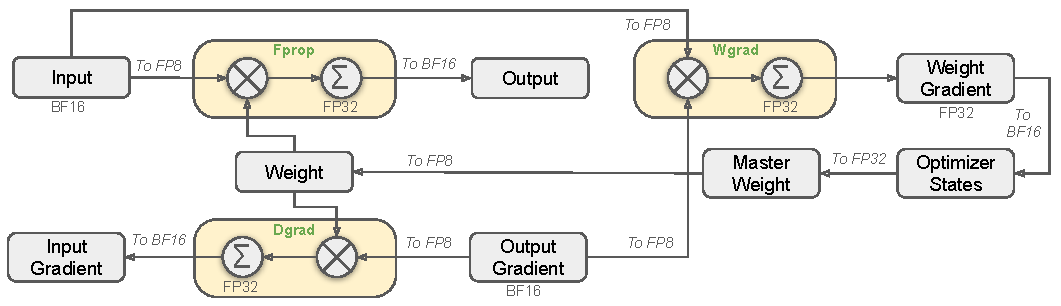
\includegraphics[width=0.99\linewidth]{figures/fp8-frameworkv3-repaired.pdf}
\caption{FP8数据格式的混合精度框架概览。为了清晰易懂,我们只画出了\texttt{线性}运算符。}
\label{fig:fp8_framework}
\end{figure}

受到最近低精度训练的研究进展的启发,我们提出了一种细粒度的混合精度框架,也就是利用FP8数据格式来训练\dsviii{}模型。尽管低精度训练具有巨大潜力,但在激活值、权重和梯度中常常存在异常值,这也限制了低精度训练的应用。尽管低精度技术在推理量化方面已取得显著进展,但关于低精度技术在大模型预训练中的成功应用的研究仍然相对较少。为了解决这个挑战并有效扩展FP8格式的动态范围,我们提出了一种细粒度的量化策略:基于$1\times N_c$元素的切片分组或基于$N_c\times N_c$元素的块分组。通过提高精度并累加的方式,我们有效缓解了与去量化(dequantization)相关的开销,这对实现准确的FP8通用矩阵乘法(GEMM)至关重要。此外,为了进一步减少MoE训练中的内存和通信开销,我们以FP8格式缓存和调度激活值,同时以BF16格式存储低精度优化器状态。我们在与\dsvii{}-Lite和\dsvii{}类似的两个模型规模上验证了所提出的FP8混合精度框架,并训练了大约1万亿个tokens(详细信息请参见附录~\ref{app:fp8_cp_bf16})。值得注意的是,与BF16基准相比,我们的FP8训练模型的相对损失误差始终保持在0.25\%以下,处于训练随机性的可接受范围内。

\subsubsection{混合精度框架}

基于广泛采用的低精度训练技术,我们提出了一种用于FP8训练的混合精度框架。在该框架中,大多数计算密集型运算使用FP8进行处理,而一些关键运算则通过策略性地保持原始数据格式,来平衡训练效率和数值稳定性。整体框架如图~\ref{fig:fp8_framework}所示。

首先,为了加速模型训练,大多数核心计算核(即GEMM操作)采用FP8精度实现。这些GEMM运算接受FP8张量作为输入,并生成BF16或FP32格式的输出。如图~\ref{fig:fp8_framework}所示,与\texttt{线性}运算相关的三个GEMM运算——\texttt{Fprop}(前向传播)、\texttt{Dgrad}(激活反向传播)和\texttt{Wgrad}(权重反向传播)——都在FP8中执行。与原始的BF16方法相比,这种设计理论上使得计算速度翻倍。此外,FP8的\texttt{Wgrad} GEMM允许激活值以FP8格式存储,并在反向传播中使用。这大大减少了内存消耗。

尽管FP8格式在效率上具有优势,但某些运算对低精度计算很敏感,所以要求更高的精度。此外,一些低成本运算也可以使用更高的精度,而对整体训练成本的影响几乎可以忽略不计。因此,在经过仔细调查后,我们决定对于以下组件保持原始精度(例如BF16或FP32):嵌入模块、输出头、MoE门控模块、归一化运算符和注意力运算符。针对性地保留高精度可以确保\dsviii{}训练过程中的稳定性。为了进一步确保数值稳定性,我们使用更高的精度存储主权重、权重梯度和优化器状态。尽管这些高精度组件会引入一些内存开销,但通过在我们的分布式训练系统中实现的高效分片技术,可以最小化它们的影响。

\begin{figure}[!t]
\centering
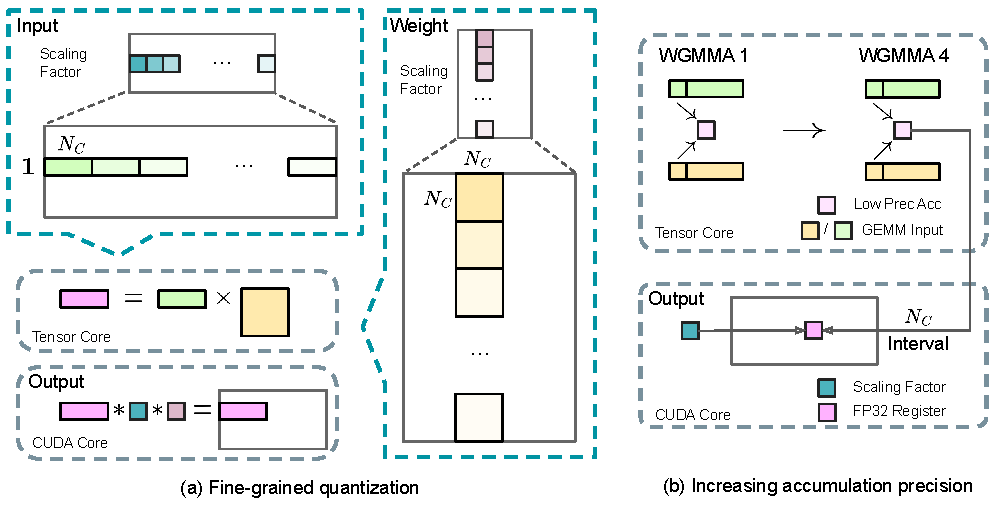
\includegraphics[width=0.95\linewidth]{figures/fp8-128accumulatorv4.pdf}
\caption{
    (a) 我们提出了一种细粒度量化方法,以减轻由异常特征值引起的量化误差;为了简单说明,仅展示了\texttt{Fprop}。(b) 配合我们的量化策略,当矩阵乘法累加运算(MMA)达到间隔$N_C=128$时,就将中间结果提升至CUDA核进行运算,从而提升了FP8 GEMM的精度,实现高精度的累加。
}
\label{fig:fp8_quantization}
\end{figure}

\subsubsection{量化和乘法带来的精度提升}

基于我们的FP8混合精度框架,我们引入了几种策略来提高低精度训练的准确性,重点优化量化方法和乘法过程。

\paragraph{细粒度的量化。}
在低精度训练框架中,由于FP8格式的动态范围有限,且其指数位数较少,溢出和下溢是常见的挑战。标准的做法是,输入分布通过将输入张量的最大绝对值缩放到FP8可表示的最大值,来对齐到FP8格式的表示范围。这种方法使得低精度训练对激活值的异常值非常敏感,而异常值可能会严重降低量化精度。为了解决这个问题,我们提出了一种细粒度的量化方法,在更细的层面上进行缩放。如图~\ref{fig:fp8_quantization}(a)所示,(1) 对于激活值,我们按\texttt{1x128}的切片方式对元素进行分组和缩放(即每个Token每128个通道);(2) 对于权重,我们按\texttt{128x128}一块的方式对元素进行分组和缩放(即每128个输入通道对128个输出通道)。这种方法确保量化过程能够根据较小的元素组调整缩放,来更好地适应异常值。在附录~\ref{app:fp8_blockwise}中,我们进一步讨论了当我们按与权重量化相同的方式对激活值进行块级分组和缩放时,可能出现的训练不稳定性。

我们方法中的一个关键修改是,顺着GEMM运算内部维度,引入了每组缩放因子。这一功能在标准的FP8 GEMM中并不直接支持,但结合我们的精确FP32累加策略,可以高效地实现。

值得注意的是,我们的细粒度量化策略与微缩放格式的理念高度一致,而NVIDIA下一代GPU(Blackwell系列)的Tensor Cores已宣布支持具有更小量化粒度的微缩放格式。这里希望我们的设计能为未来的工作提供参考,以跟上最新GPU架构的发展。

\paragraph{提高累加精度。}
低精度GEMM运算常常遭遇下溢问题,它们的精度在很大程度上依赖于高精度的累加,而这通常是在FP32精度下进行的。然而,我们观察到,在NVIDIA H800 GPU上,FP8 GEMM的累加精度仅能保留大约14位,这明显低于FP32的累加精度。当内部维度\texttt{K}较大时,这个问题会变得更加明显,因为在大模型训练的典型场景中,批大小和模型宽度都会增大。以\texttt{K} = 4096的两个随机矩阵的GEMM运算为例,在初步测试中,Tensor Cores中有限的累加精度导致最大相对误差接近2\%。尽管存在这些问题,有限的累加精度仍然是一些FP8框架中的默认选项,这严重制约了训练的准确性。

为了解决这个问题,我们采用了\underline{提升到CUDA核进行运算}的方法以获得更高的精度。这一过程如图~\ref{fig:fp8_quantization}(b)所示。具体来说,在张量核(Tensor Cores)上执行MMA(矩阵乘法累加)时,使用有限的位宽累加中间结果。一旦达到$N_C$的间隔,将这些中间结果复制到CUDA核上的FP32寄存器中,并在那里执行全精度的FP32累加。如前所述,我们的细粒度量化在内部维度\texttt{K}上应用每组缩放因子。这些缩放因子可以在CUDA核上高效地与去量化过程一起进行乘法运算,且几乎没有额外的计算开销。

值得注意的是,这一修改减少了单个warpgroup的WGMMA(warp组级别矩阵乘法累加)指令发射率。然而,在H800架构上,通常会有两个WGMMA并行存在:一个warpgroup执行提升操作,另一个则执行MMA运算。这种设计使得两个操作能够重叠执行,从而保持了张量核的高利用率。根据我们的实验,将$N_C=128$元素(相当于4个WGMMAs)设置为最小的累加间隔,可以显著提高精度,同时不会引入过多的开销。

\paragraph{尾数优于指数。}
先前NVIDIA某项工作采用了混合FP8格式,也就是在\texttt{Fprop}中使用\texttt{E4M3}(4位指数和3位尾数),在\texttt{Dgrad}和\texttt{Wgrad}中使用\texttt{E5M2}(5位指数和2位尾数)。而我们选择了不同的策略,我们在所有张量中都采用\texttt{E4M3}格式,以获得更高的精度。我们认为这种方法可行的原因在于我们的细粒度量化策略,即切片级别和块级别的缩放。通过对较小的元素组进行运算,我们的方法有效地在这些分组元素之间共享指数位,从而减轻了有限动态范围的影响。

\paragraph{在线量化。}
延迟量化被应用于张量级量化框架中,该框架维护了先前迭代中最大绝对值的历史记录,以推测当前值。为了确保准确的缩放因子并简化框架,我们对每个\texttt{1x128}激活切片或\texttt{128x128}权重块在线计算最大绝对值。基于该值,我们推导出缩放因子,然后在线将激活值或权重量化为FP8格式。

\subsubsection{低精度数据的存储和通信}

结合我们的FP8训练框架,通过将缓存的激活值和优化器状态压缩为低精度格式,进一步减少了内存消耗和通信开销。

\paragraph{低精度优化器状态。}
我们采用BF16数据格式而不是FP32来跟踪AdamW优化器中的一阶和二阶矩,且没有引起明显的性能下降。然而,主权重(由优化器存储)和梯度(用于批量大小累加)仍然使用FP32,以确保整个训练过程中的数值稳定性。

\paragraph{低精度激活值。}
如图~\ref{fig:fp8_framework}所示,\texttt{Wgrad}运算使用FP8执行。为了减少内存消耗,在\texttt{线性}运算的反向传播中,将激活值缓存为FP8格式是一个自然的选择。然而,针对一些运算,我们在低成本高精度训练中进行了特别考虑:

\begin{quote}
\textbf{(1) 注意力运算符后面的\texttt{线性}输入。} 这些激活值也用于注意力运算符的反向传播,因此对精度比较敏感。我们为这些激活值采用了定制的\texttt{E5M6}数据格式。此外,这些激活值将在反向传播中从\texttt{1x128}量化切片转换为\texttt{128x1}切片。为了避免引入额外的量化误差,所有的缩放因子都采用2的整数次幂进行四舍五入缩放。

\textbf{(2) MoE中的SwiGLU运算符的输入。} 为了进一步降低内存开销,我们缓存SwiGLU运算符的输入,并在反向传播中重新计算其输出。这些激活值也使用我们的细粒度量化方法以FP8格式存储,在内存效率和计算精度之间取得平衡。
\end{quote}

\paragraph{低精度数据的通信。}
通信带宽是MoE模型训练中的一个关键瓶颈。为了缓解这一挑战,我们将MoE上投影前的激活值量化为FP8,然后应用\texttt{dispatch}组件,这与MoE上投影中的FP8 \texttt{Fprop}兼容。与注意力运算符后面的\texttt{线性}输入类似,这些激活值的缩放因子是2的整数次幂。类似的策略也应用于MoE下投影前的激活梯度。对于前向和反向的\texttt{combine}组件,我们将它们保留为BF16,以确保训练过程中关键部分的训练精度。

\subsection{推理和部署}
\label{sec:inference_deployment}

我们在H800集群上部署了\dsviii{},其中每个节点内的GPU通过NVLink互连,集群内所有GPU通过 InfiniBand 实现全互连。为了同时确保在线服务的服务级目标(SLO)和高吞吐量,我们采用了以下部署策略,将\textit{预填充}和\textit{解码}阶段分开。

\subsubsection{预填充(Prefilling)}

预填充阶段的最小部署单元由4个节点和32个GPU组成。\texttt{attention}部分采用4路张量并行(TP4)与序列并行(SP)相结合,再加上8路数据并行(DP8)。其较小的张量并行大小为4,限制了张量并行的通信开销。对于\texttt{MoE}部分,我们使用32路专家并行(EP32),确保每个专家处理足够大的批次大小,从而提高计算效率。对于\texttt{MoE}的All-to-All通信,我们采用与训练相同的方法:首先通过 InfiniBand 在节点间传输Token,然后通过 NVLink 在节点内的GPU之间转发。特别地,对于浅层中的稠密MLP,我们使用1路张量并行,以节省张量并行的通信开销。

为了在\texttt{MoE}部分实现不同专家之间的负载均衡,我们需要确保每个GPU处理大致相同数量的Token。为此,我们引入了一种\textit{冗余专家}的部署策略,复制高负载专家并进行冗余部署。高负载专家是根据在线部署过程中收集的统计信息检测到的,并定期进行调整(例如,每10分钟调整一次)。在确定冗余专家集合后,我们根据观察到的负载,仔细地在一个节点内重新安排专家,尽量在不增加跨节点All-to-All通信开销的情况下均衡各GPU的负载。对于\dsviii{}的部署,我们在预填充阶段设置了32个冗余专家。对于每个GPU,除了原有的8个专家外,还将托管一个额外的冗余专家。

此外,在预填充阶段,为了提高吞吐量并隐藏All-to-All和张量并行通信的开销,我们同时处理两个具有相似计算负载的微批次,将一个微批次的\texttt{attention}和\texttt{MoE}与另一个微批次的\texttt{dispatch}和\texttt{combine}重叠执行。

最后,我们正在探索一种\textit{动态冗余}策略,针对专家,每个GPU托管更多的专家(例如,16个专家),但每次推理步骤中仅激活9个专家。在每层的All-to-All操作开始之前,我们即时计算全局最优的路由方案。鉴于预填充阶段涉及的大量计算,计算这个路由方案的开销几乎可以忽略不计。

\subsubsection{解码}

在解码过程中,我们将共享专家视为路由专家。从这个角度来看,每个Token在路由过程中将选择9个专家,其中共享专家被视为高负载专家,将始终被选择。解码阶段的最小部署单元由40个节点和320个GPU组成。\texttt{attention}部分采用4路张量并行(TP4)与序列并行(SP)相结合,再配合80路数据并行,而\texttt{MoE}部分使用320路专家并行。对于\texttt{MoE}部分,每个GPU只托管一个专家,64个GPU负责托管冗余专家和共享专家。\texttt{dispatch}和\texttt{combine}部分的All-to-All通信通过 InfiniBand 进行直接点对点传输,以实现低延迟。此外,我们利用IBGDA技术进一步最小化延迟并提高通信效率。

与预填充阶段类似,我们根据在线服务中的专家负载统计,定期确定冗余专家集合。然而,由于每个GPU只托管一个专家,我们不需要重新安排专家。我们还在探索解码阶段的\textit{动态冗余}策略,但这需要更仔细地优化计算全局最优路由方案的算法,并与\texttt{dispatch}核进行融合以减少开销。

此外,为了提高吞吐量并隐藏All-to-All通信的开销,我们还在探索在解码阶段同时处理两个具有相似计算负载的微批次。与预填充阶段不同,\texttt{attention}在解码阶段消耗了较大部分的时间。因此,我们将一个微批次的\texttt{attention}与另一个微批次的\texttt{dispatch+MoE+combine}重叠执行。在解码阶段,每个专家的批次大小相对较小(通常在256个Token以内),瓶颈是内存访问而非计算。由于\texttt{MoE}部分只需要加载一个专家的参数,因此内存访问开销最小,因此使用较少的流式多处理器不会显著影响整体性能。因此,为了避免影响\texttt{attention}部分的计算速度,我们可以将少部分流式多处理器分配给\texttt{dispatch+MoE+combine}部分。

\subsection{对硬件设计的建议}
\label{fp8_hardware_design}

基于我们在实现All-to-All通信和FP8训练策略时的经验,我们想对AI硬件提供商提出以下设计芯片的建议:

\subsubsection{通信硬件}

在 \dsviii{} 中,我们通过在计算过程中隐藏通信延迟来实现计算与通信的重叠。这显著减少了与串行计算和通信相比对通信带宽的依赖。然而,目前的通信实现依赖于昂贵的流式多处理器(例如,我们为此在H800 GPU中分配了132个流式多处理器中的20个),这将限制计算吞吐量。此外,使用流式多处理器进行通信会导致显著的低效,因为张量核完全没有得到充分利用。

目前,在All-to-All通信中,流式多处理器主要执行以下任务:

\begin{itemize}[topsep=0pt]
    \item
    \textbf{在 InfiniBand 和 NVLink 域之间转发数据},同时汇聚从单个 GPU 发往同一节点内多个 GPU 的 InfiniBand 流量。
    \item 
    \textbf{在 RDMA 缓冲区(已注册的 GPU 内存区域)和输入/输出缓冲区之间传输数据}。
    \item 
    \textbf{执行 \texttt{reduce} 运算},用于 \texttt{all-to-all} \texttt{combine}。
    \item
    \textbf{在通过 InfiniBand 和 NVLink 域向多个专家传输分块数据时,管理细粒度的内存布局}。
\end{itemize}

我们期望未来的硬件供应商能够开发出将这些通信任务从宝贵的计算单元 流式多处理器 中卸载的硬件,作为 GPU 协处理器或类似 NVIDIA SHARP 的网络协处理器。此外,为了降低应用程序编程的复杂性,我们希望该硬件能够从计算单元的角度统一 InfiniBand(扩展)和 NVLink(扩展)网络。通过这个统一接口,计算单元可以轻松地通过提交基于简单原语的通信请求,完成诸如 \texttt{read}、\texttt{write}、\texttt{multicast} 和 \texttt{reduce} 等操作,跨越整个 InfiniBand-NVLink-统一域。

\subsubsection{计算硬件}

\paragraph{张量核中更高的 FP8 GEMM 累加精度。}
在 NVIDIA Hopper 架构的张量核实现中,FP8 GEMM(通用矩阵乘法)采用定点累加,在加法之前通过基于最大指数的右移对尾数积进行对齐。我们的实验表明,在符号填充右移后,它仅使用每个尾数积的最高 14 位,并截断超过此范围的位。然而,例如,为了从 32 次 FP8$\times$FP8 相乘的累加中获得精确的 FP32 结果,至少需要 34 位精度。因此,我们建议未来的芯片设计在张量核中提高累加精度,以支持全精度累加,或根据训练和推理算法的精度需求选择适当的累加位宽。这种方法可以确保误差保持在可接受的范围内,同时保持计算效率。

\paragraph{支持Tile级和块级量化。}
目前的GPU仅支持张量级别的量化,缺乏对像我们这种Tile级别和块级别量化的原生支持。在当前的实现中,当达到$N_C$间隔时,部分结果会从张量核复制到CUDA核,乘以缩放因子后,添加到CUDA核上的FP32寄存器中。尽管结合我们精确的FP32累加策略,去量化开销已经得到了显著缓解,但频繁的张量核和CUDA核之间的数据移动仍然限制了计算效率。因此,我们建议未来的芯片支持细粒度量化,通过使张量核能够接收缩放因子并实现带组缩放的MMA(矩阵乘法累加)。这样,整个部分和累加去量化的过程可以直接在张量核内部完成,直到最终结果产生,从而避免频繁的数据移动。

\paragraph{支持在线量化。}
尽管我们的研究已证明在线量化的有效性,当前的实现仍难以有效支持在线量化。在现有过程中,我们需要从HBM(高带宽内存)中读取128个BF16激活值(上一步计算的输出)进行量化,然后将量化后的FP8值写回到HBM,再次读取用于MMA。为了解决这一低效问题,我们建议未来的芯片将FP8类型转换和TMA(张量内存加速器)访问集成为一个融合操作,这样量化过程可以在激活值从全局内存传输到共享内存的过程中完成,从而避免频繁的内存读写操作。我们还建议支持一个Warp级的类型转换指令,以加速运算,并进一步促进层归一化和FP8类型转换的更好融合。另外,也可以采用近内存计算的方法,将计算逻辑放置在靠近HBM的位置。在这种情况下,BF16元素可以在从HBM读取到GPU时直接转换为FP8,减少大约50\%的芯片外内存访问。

\paragraph{支持转置GEMM运算。}
当前的架构使得将矩阵转置与GEMM运算融合变得繁琐。在我们的工作流程中,前向传播过程中,激活值被量化为\texttt{1x128}的FP8 Tile并存储。在反向传播过程中,矩阵需要被读取、去量化、转置、重新量化为\texttt{128x1} Tile,并存储在HBM中。为了减少内存操作,我们建议未来的芯片在执行MMA运算之前,允许从共享内存中直接读取转置后的矩阵,适用于训练和推理所需的精度。结合FP8格式转换与TMA访问的融合,这一增强将显著简化量化工作流程。

\section{预训练(Pre-Training)}
\label{sec:pre-training}

\subsection{训练数据的构成}

与 \dsvii{} 相比,我们通过增强数学和编程样本的比例来优化预训练语料库,同时扩展了多语言覆盖范围,超越了英语和中文。此外,我们的数据处理流水线经过改进,以最小化冗余,同时保持语料库的多样性。受 Ding2024FewerTI 的启发,我们实现了文档打包方法以确保数据完整性,但在训练过程中未采用跨样本注意力掩码。最后,\dsviii{} 的训练语料库由 14.8T 高质量和多样化的Token组成。

在 DeepSeekCoder-V2 的训练过程中,我们观察到填充中间(Fill-in-Middle,FIM)策略并未损害下一个Token预测能力,同时使模型能够基于上下文线索准确预测中间文本。与 DeepSeekCoder-V2 一致,我们在 \dsviii{} 的预训练中也采用了 FIM 策略。具体来说,我们使用前缀-后缀-中间(Prefix-Suffix-Middle,PSM)框架来构建数据,如下所示:

\begin{align}
\texttt{<|fim\_begin|>}f_{\text{pre}}\texttt{<|fim\_hole|>}f_{\text{suf}}\texttt{<|fim\_end|>}f_{\text{middle}}\texttt{<|eos\_token|>} . \nonumber
\end{align}

该结构在文档级别应用,作为预打包过程的一部分。FIM 策略的应用比例为 0.1,符合 PSM 框架。

\dsviii{} 的分词器采用字节级 BPE 分词器,并将词汇表扩展为 128K 个Token。分词器的预分词器和训练数据经过修改,以优化多语言压缩效率。此外,与 \dsvii{} 相比,新的预分词器引入了将标点符号和换行符结合的Token。然而,当模型处理没有终止换行符的多行提示时,这种技巧可能会引入Token边界偏差,特别是在少样本评估提示中。为了解决这个问题,我们在训练过程中随机拆分一定比例的这种组合Token,从而使模型接触到更广泛的特殊情况,并减轻这种偏差。

\subsection{超参数}

\paragraph{模型超参数。}
我们将Transformer层数设置为61,隐藏层维度设置为7168。所有可学习参数的初始化标准差为0.006。在\dsattn{}中,我们将注意力头数$n_h$设置为128,每个头的维度$d_h$设置为128。KV压缩维度$d_c$设置为512,查询压缩维度$d_c^{\prime}$设置为1536。对于解耦查询和解耦键,我们将每个头的维度$d_h^R$设置为64。我们将除了前三层之外的所有前馈网络替换为MoE层。每个MoE层包含1个共享专家和256个路由专家,每个专家的中间隐藏层维度为2048。在路由专家中,每个Token将激活8个专家,每个Token将确保最多发送到4个节点。多Token预测深度$D$设置为1,即除了精确的下一个Token外,每个Token还会预测一个额外的Token。与\dsvii{}类似,\dsviii{}也在压缩后的潜在向量后使用额外的RMSNorm层,并在宽度瓶颈处乘以额外的缩放因子。在此配置下,\dsviii{}包含671B总参数,其中每个Token激活的参数为37B。

\paragraph{训练超参数。}
我们采用AdamW优化器,超参数设置为$\beta_1=0.9$,$\beta_2=0.95$,以及$\mathrm{weight\_decay}=0.1$。在预训练期间,我们将最大序列长度设置为4K,并在14.8T个Token上进行预训练\dsviii{}。关于学习率调度,我们首先在前2K步内将学习率从0线性增加到$2.2 \times 10^{-4}$。然后,我们保持学习率为$2.2 \times 10^{-4}$,直到模型处理了10T个训练Token。接下来,我们将学习率逐渐衰减至$2.2 \times 10^{-5}$,在4.3T个Token内按余弦衰减曲线进行衰减。在最后500B Token的训练过程中,我们在前333B Token内保持学习率为$2.2 \times 10^{-5}$不变,并在剩余的167B Token内切换为$7.3 \times 10^{-6}$的常数学习率。梯度裁剪范数设置为1.0。我们采用批次大小调度策略,在训练的前469B Token中,批次大小逐渐从3072增加到15360,之后在剩余训练中保持15360。我们利用流水线并行将模型的不同层部署到不同的GPU上,对于每一层,路由专家将均匀地部署在64个GPU上,这些GPU属于8个节点。关于限制了节点数量的路由,每个Token最多将被发送到4个节点(即$M=4$)。为了实现无辅助损失的负载均衡,我们将偏置更新速度$\gamma$设置为0.001,适用于前14.3T个Token,在剩余的500B Token中设置为0.0。对于平衡损失,我们将$\alpha$设置为0.0001,以避免单个序列内出现极端不均衡。MTP损失权重$\lambda$在前10T Token中设置为0.3,在剩余的4.8T Token中设置为0.1。

\begin{figure}[h]
    \centering
    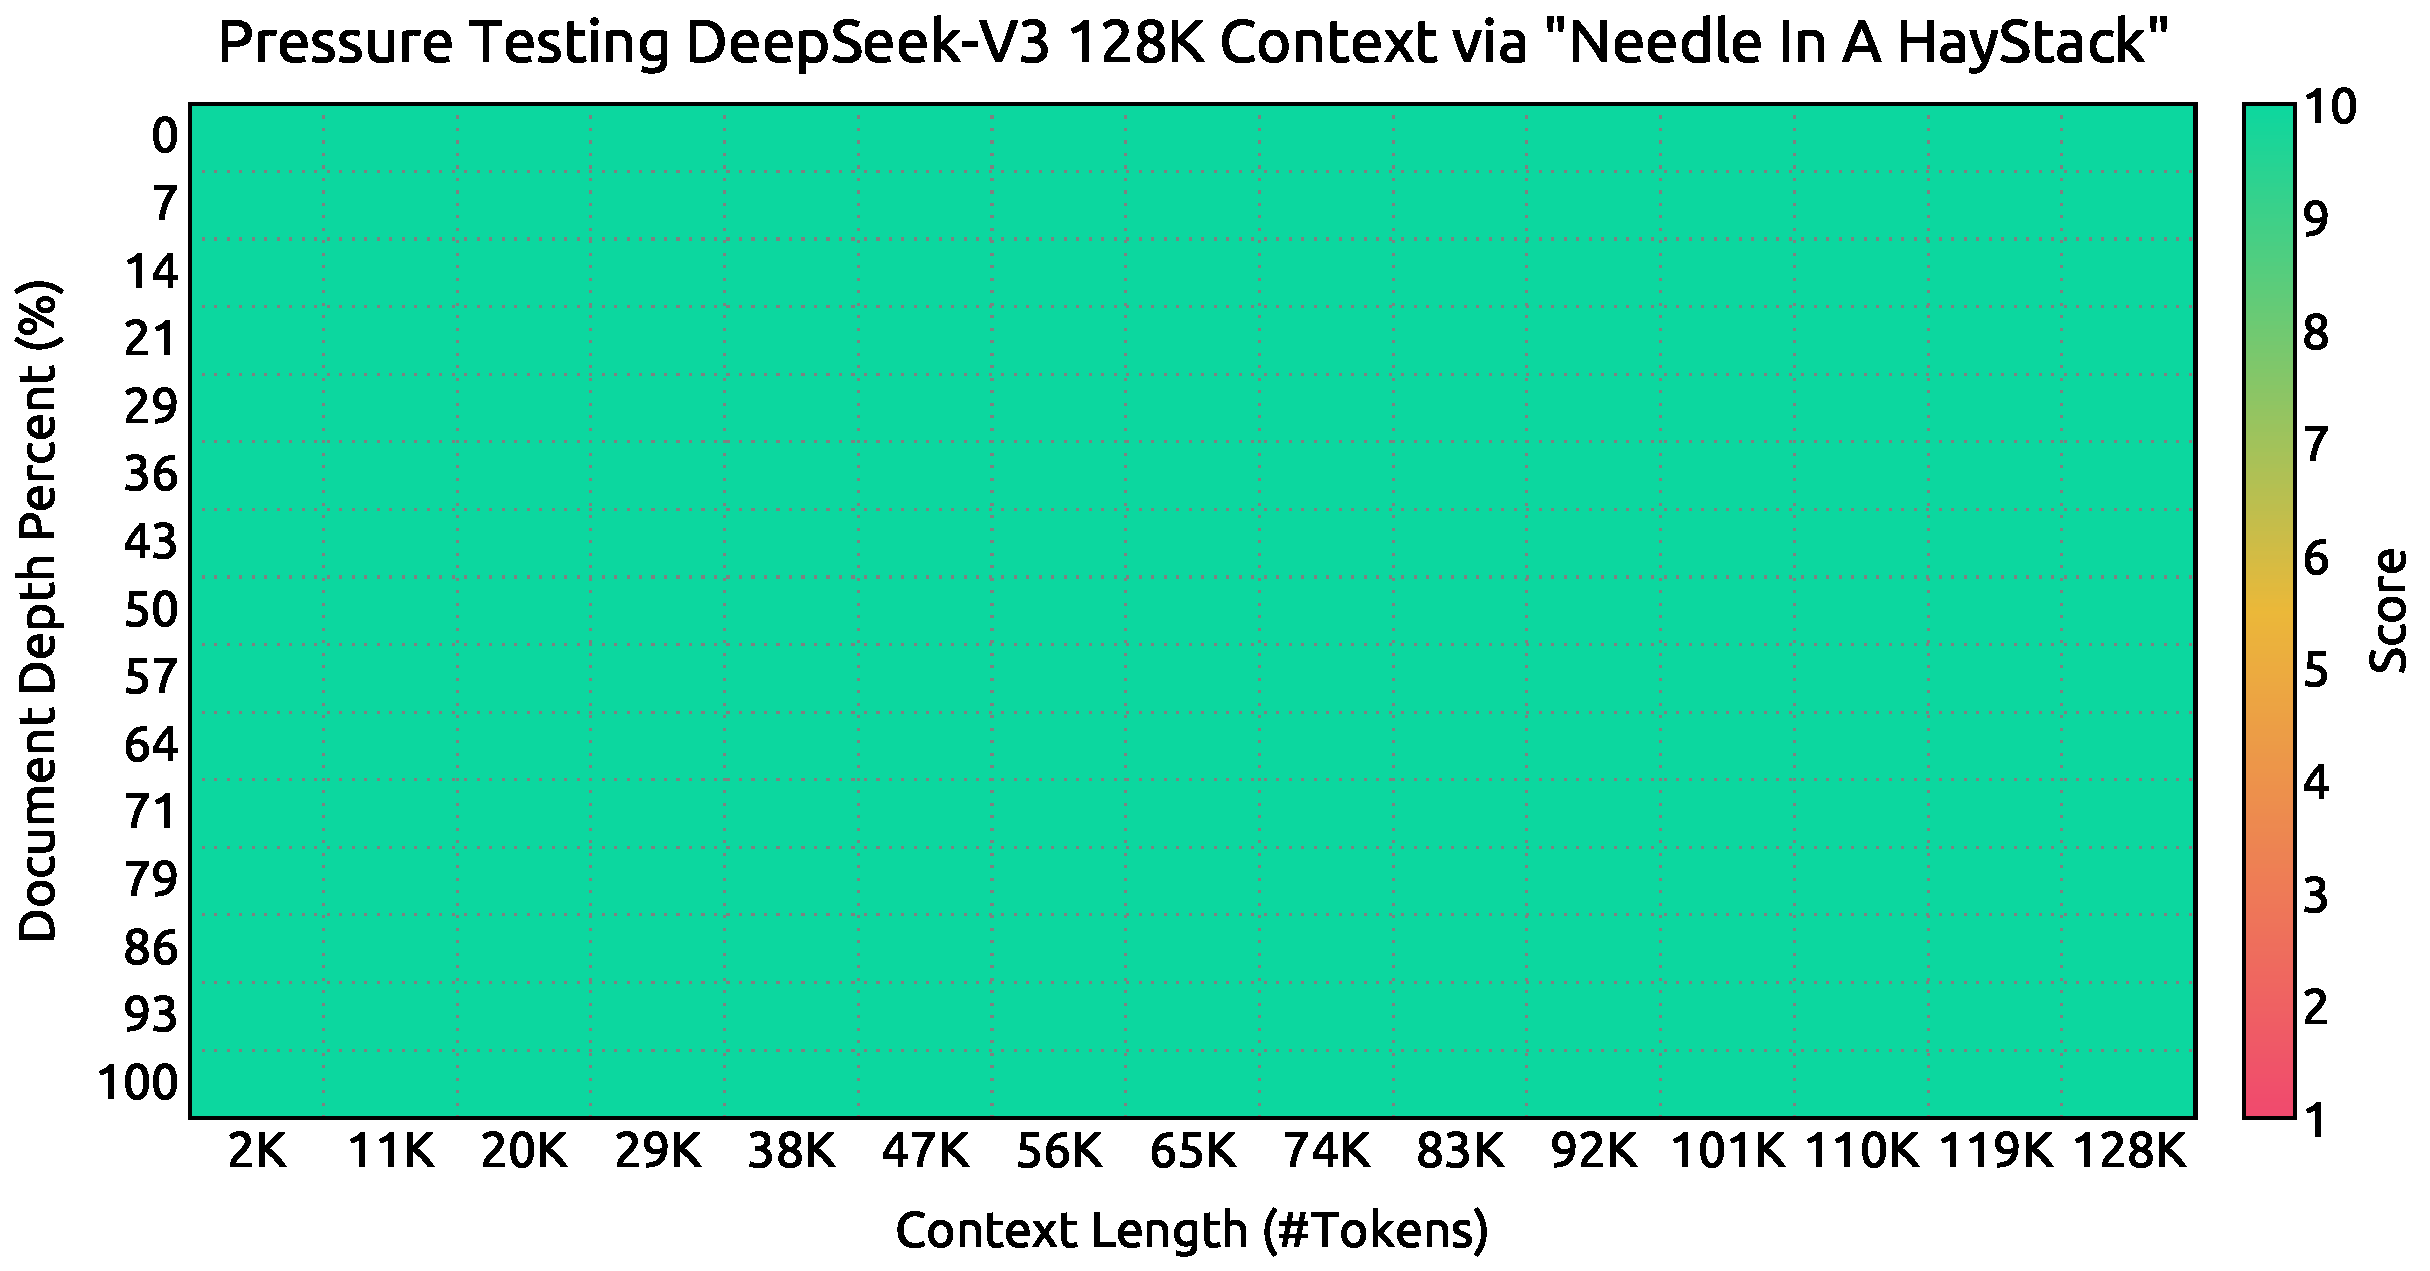
\includegraphics[width=0.98\linewidth]{figures/needle_in_a_haystack.pdf}
    \caption{
        在 ''Needle In A Haystack'' (NIAH) 测试集上的评估结果。\dsviii{} 在 128K 以内的上下文窗口长度下,都表现很好。
    }
    \label{fig:long_context}
\end{figure}

\subsection{长上下文扩展}

我们采用与\dsvii{}类似的方法,在\dsviii{}中实现长上下文能力。在预训练阶段之后,我们使用YaRN进行上下文扩展,并执行两个额外的训练阶段,每个阶段包括1000步,逐步将上下文窗口从4K扩展到32K,再扩展到128K。YaRN的配置与在\dsvii{}中使用的配置一致,仅应用于解耦共享键$\mathbf{k}^R_t$。两个阶段的超参数保持相同,分别为:比例因子$s = 40$,$\alpha = 1$,$\beta = 32$,以及缩放因子$\sqrt{t} = 0.1 \ln{s} + 1$。在第一个阶段,序列长度设置为32K,批次大小为1920。在第二个阶段,序列长度增加到128K,批次大小减少到480。两个阶段的学习率都设置为$7.3 \times 10^{-6}$,与预训练阶段的最终学习率相匹配。  

通过这两阶段的扩展训练,\dsviii{}能够处理最大长度为128K的输入,并保持强大的性能。图~\ref{fig:long_context}展示了经过监督微调后的\dsviii{}在"Needle In A Haystack"(NIAH)测试中取得了显著的表现,且在上下文窗口长度达到128K时,展现了持续的健壮性。

\subsection{评估}

\subsubsection{评估基准}

\dsviii{} 的基础模型是在一个多语言语料库上进行预训练的,其中英语和中文占据了大多数。因此,我们对其在一系列基准测试中的表现进行了评估,这些基准测试主要是英语和中文,以及一个多语言基准。我们的评估基于集成在我们的 HAI-LLM 框架中的内部评估框架。基准被分类并列出如下,其中:带\underline{下划线}的基准为中文基准,带\uuline(双下划线)的基准为多语言基准:

\textbf{多学科多项选择} 数据集包括 MMLU、MMLU-Redux、MMLU-Pro、\uuline{MMMLU}、\underline{C-Eval} 和 \underline{CMMLU}。

\textbf{语言理解与推理} 数据集包括 HellaSwag、PIQA、ARC 和 BigBench Hard (BBH)。

\textbf{闭卷问答} 数据集包括 TriviaQA 和 NaturalQuestions。

\textbf{阅读理解} 数据集包括 RACE、DROP、\underline{C3} 和 \underline{CMRC}。

\textbf{参考消歧} 数据集包括 \underline{CLUEWSC} 和 WinoGrande 。

\textbf{语言建模} 数据集包括 Pile 。

\textbf{中文理解与文化} 数据集包括 \underline{CCPM} 。

\textbf{数学} 数据集包括 GSM8K、MATH、MGSM 和 \underline{CMath} 。

\textbf{代码} 数据集包括 HumanEval、LiveCodeBench-Base (0801-1101)、MBPP 和 CRUXEval。

\textbf{标准化考试} 包括 \underline{AGIEval} 。请注意,AGIEval 包括英语和中文两个子集。

根据我们之前的工作,我们对以下数据集采用基于困惑度的评估:HellaSwag、PIQA、WinoGrande、RACE-Middle、RACE-High、MMLU、MMLU-Redux、MMLU-Pro、MMMLU、ARC-Easy、ARC-Challenge、C-Eval、CMMLU、C3 和 CCPM;对于 TriviaQA、NaturalQuestions、DROP、MATH、GSM8K、MGSM、HumanEval、MBPP、LiveCodeBench-Base、CRUXEval、BBH、AGIEval、CLUEWSC、CMRC 和 CMath,我们采用基于生成的评估。此外,我们对 Pile-test 进行基于语言建模的评估,并使用每字节比特数(Bits-Per-Byte, BPB)作为指标,以确保在使用不同分词器的模型之间进行公平比较。

\begin{table}[!h]
    \centering
    \footnotesize
    \setlength{\tabcolsep}{4.5pt}
    \begin{tabular}{@{}c l c | c | c c | c@{}}
    \toprule
    & \multirow{2}{*}{\centering \textbf{Benchmark {\tiny (Metric)}}} & \multirow{2}{*}{\textbf{\# Shots}} & \textbf{\dsvii{}} & \textbf{Qwen2.5} & \textbf{LLaMA-3.1} & \textbf{\dsviii{}} \\
    & & & \textbf{Base} & \textbf{72B Base} & \textbf{405B Base} & \textbf{Base} \\
    \midrule
    & Architecture & - & MoE & Dense & Dense & MoE \\
    & \# Activated Params & - & 21B & 72B & 405B & 37B \\
    & \# Total Params & - & 236B & 72B & 405B & 671B \\
    \midrule
    \multirow{16}{*}{English} & Pile-test {\tiny (BPB)} & - & 0.606 & 0.638 & \textbf{0.542} & 0.548 \\
    & BBH {\tiny (EM)} & 3-shot & 78.8 & 79.8 & 82.9 & \textbf{87.5} \\
    & MMLU {\tiny (EM)} & 5-shot & 78.4 & 85.0 & 84.4 & \textbf{87.1} \\
    & MMLU-Redux {\tiny (EM)} & 5-shot & 75.6 & 83.2 & 81.3 & \textbf{86.2} \\
    & MMLU-Pro {\tiny (EM)} & 5-shot & 51.4 & 58.3 & 52.8 & \textbf{64.4} \\
    & DROP {\tiny (F1)} & 3-shot & 80.4 & 80.6 & 86.0 & \textbf{89.0} \\
    & ARC-Easy {\tiny (EM)} & 25-shot & 97.6 & 98.4 & 98.4 & \textbf{98.9} \\
    & ARC-Challenge {\tiny (EM)} & 25-shot & 92.2 & 94.5 & \textbf{95.3} & \textbf{95.3} \\
    & HellaSwag {\tiny (EM)} & 10-shot & 87.1 & 84.8 & \textbf{89.2} & \textbf{88.9} \\
    & PIQA {\tiny (EM)} & 0-shot & 83.9 & 82.6 & \textbf{85.9} & 84.7 \\
    & WinoGrande {\tiny (EM)} & 5-shot & \textbf{86.3} & 82.3 & 85.2 & 84.9 \\
    & RACE-Middle {\tiny (EM)} & 5-shot & 73.1 & 68.1 & \textbf{74.2} & 67.1 \\
    & RACE-High {\tiny (EM)} & 5-shot & 52.6 & 50.3 & \textbf{56.8} & 51.3 \\
    & TriviaQA {\tiny (EM)} & 5-shot & 80.0 & 71.9 & \textbf{82.7} & \textbf{82.9} \\
    & NaturalQuestions {\tiny (EM)} & 5-shot & 38.6 & 33.2 & \textbf{41.5} & 40.0 \\
    & AGIEval {\tiny (EM)} & 0-shot & 57.5 & 75.8 & 60.6 & \textbf{79.6} \\
    \midrule
    \multirow{4}{*}{Code} & HumanEval {\tiny (Pass@1)} & 0-shot & 43.3 & 53.0 & 54.9 & \textbf{65.2} \\
    & MBPP {\tiny (Pass@1)} & 3-shot & 65.0 & 72.6 & 68.4 & \textbf{75.4} \\
    & LiveCodeBench-Base {\tiny (Pass@1)} & 3-shot & 11.6 & 12.9 & 15.5 & \textbf{19.4} \\
    & CRUXEval-I {\tiny (EM)} & 2-shot & 52.5 & 59.1 & 58.5 & \textbf{67.3} \\
    & CRUXEval-O {\tiny (EM)} & 2-shot & 49.8 & 59.9 & 59.9 & \textbf{69.8} \\
    \midrule
    \multirow{3}{*}{Math} & GSM8K {\tiny (EM)} & 8-shot & 81.6 & 88.3 & 83.5 & \textbf{89.3} \\
    & MATH {\tiny (EM)} & 4-shot & 43.4 & 54.4 & 49.0 & \textbf{61.6} \\
    & MGSM {\tiny (EM)} & 8-shot & 63.6 & 76.2 & 69.9 & \textbf{79.8} \\
    & CMath {\tiny (EM)} & 3-shot & 78.7 & 84.5 & 77.3 & \textbf{90.7} \\
    \midrule
    \multirow{7}{*}{Chinese} & CLUEWSC {\tiny (EM)} & 5-shot & 82.0 & 82.5 & \textbf{83.0} & \textbf{82.7} \\
    & C-Eval {\tiny (EM)} & 5-shot & 81.4 & 89.2 & 72.5 & \textbf{90.1} \\
    & CMMLU {\tiny (EM)} & 5-shot & 84.0 & \textbf{89.5} & 73.7 & 88.8 \\
    & CMRC {\tiny (EM)} & 1-shot & \textbf{77.4} & 75.8 & 76.0 & 76.3 \\
    & C3 {\tiny (EM)} & 0-shot & 77.4 & 76.7 & \textbf{79.7} & 78.6 \\
    & CCPM {\tiny (EM)} & 0-shot & \textbf{93.0} & 88.5 & 78.6 & 92.0 \\
    \midrule
    \multirow{1}{*}{Multilingual} & MMMLU-non-English {\tiny (EM)} & 5-shot & 64.0 & 74.8 & 73.8 & \textbf{79.4} \\
    \bottomrule
    \end{tabular}
    \caption{\dsviii{}-Base 与其他代表性的开源基础模型的比较。所有模型在我们的内部框架中进行评估,并共享相同的评估设置。得分差距不超过 0.3 的模型被认为处于同一水平。\dsviii{}-Base 在大多数基准测试中表现最佳,特别是在数学和代码任务上。}
    \label{tab:main}
\end{table}

\subsubsection{评估结果}

在表~\ref{tab:main}中,我们将 \dsviii{} 的基础模型与最先进的开源基础模型进行比较,包括 \dsvii{}-Base(我们之前发布的版本)、Qwen2.5 72B Base 和 LLaMA-3.1 405B Base。我们使用内部评估框架对所有这些模型进行评估,并确保它们共享相同的评估设置。请注意,由于我们评估框架在过去几个月中的变化,\dsvii{}-Base 的性能与我们之前报告的结果略有不同。总体而言,\dsviii{}-Base 在各项基准测试中全面超越了 \dsvii{}-Base 和 Qwen2.5 72B Base,并在大多数基准测试中超过了 LLaMA-3.1 405B Base,基本上成为了最强的开源模型。

从更详细的角度来看,我们分别将 \dsviii{}-Base 与其他开源基础模型进行比较。

\begin{enumerate}
\item 相较于 \dsvii{}-Base,由于我们模型架构的改进、模型规模和训练Token数量的扩大,以及数据质量的提升,\dsviii{}-Base 的性能显著提高,这也是意料之中的结果。
\item 与最先进的中文开源模型 Qwen2.5 72B Base 相比,尽管激活参数只有一半,\dsviii{}-Base 在英语、多语言、代码和数学基准测试上也展现出显著优势。至于中文基准,除了 CMMLU(一个中文多学科多项选择任务),\dsviii{}-Base 的表现也优于 Qwen2.5 72B。
\item 与激活参数多达 11 倍的最大开源模型 LLaMA-3.1 405B Base 相比,\dsviii{}-Base 在多语言、代码和数学基准测试上也表现得更好。在英语和中文语言基准上,\dsviii{}-Base 的表现具有竞争力或更好,尤其在 BBH、MMLU 系列、DROP、C-Eval、CMMLU 和 CCPM 上表现突出。
\end{enumerate}

由于我们的高效架构和全面的工程优化,\dsviii{} 实现了极高的训练效率。在我们的训练框架和基础设施下,训练 \dsviii{} 每万亿个Token仅需 180K H800 GPU 小时,这比训练 72B 或 405B 这样的稠密模型便宜得多。

\begin{table}[h]
    \centering
    \footnotesize
    \setlength{\tabcolsep}{8pt}
    \begin{tabular}{@{}l c | c c | c c@{}}
    \toprule
    \multirow{2}{*}{\centering \textbf{Benchmark (Metric)}} & \multirow{2}{*}{\textbf{\# Shots}} & \textbf{Small MoE} & \textbf{Small MoE} & \textbf{Large MoE} & \textbf{Large MoE} \\
     & & \textbf{Baseline} & \textbf{w/ MTP} & \textbf{Baseline} & \textbf{w/ MTP} \\
    \midrule
    \# Activated Params {\tiny (Inference)} & - & 2.4B & 2.4B & 20.9B & 20.9B \\
    \# Total Params {\tiny (Inference)} & - & 15.7B & 15.7B & 228.7B & 228.7B \\
    \# Training Tokens & - & 1.33T & 1.33T & 540B & 540B \\
    \midrule
    Pile-test {\tiny (BPB)} & - & \textbf{0.729} & \textbf{0.729} & 0.658 & \textbf{0.657} \\
    BBH {\tiny (EM)} & 3-shot & 39.0 & \textbf{41.4} & 70.0 & \textbf{70.7} \\
    MMLU {\tiny (EM)} & 5-shot & 50.0 & \textbf{53.3} & \textbf{67.5} & 66.6 \\
    DROP {\tiny (F1)} & 1-shot & 39.2 & \textbf{41.3} & 68.5 & \textbf{70.6} \\
    TriviaQA {\tiny (EM)} & 5-shot & 56.9 & \textbf{57.7} & \textbf{67.0} & \textbf{67.3} \\
    NaturalQuestions {\tiny (EM)} & 5-shot & \textbf{22.7} & 22.3 & 27.2 & \textbf{28.5} \\
    HumanEval {\tiny (Pass@1)} & 0-shot & 20.7 & \textbf{26.8} & 44.5 & \textbf{53.7} \\
    MBPP {\tiny (Pass@1)} & 3-shot & 35.8 & \textbf{36.8} & 61.6 & \textbf{62.2} \\
    GSM8K {\tiny (EM)} & 8-shot & 25.4 & \textbf{31.4} & 72.3 & \textbf{74.0} \\
    MATH {\tiny (EM)} & 4-shot & 10.7 & \textbf{12.6} & 38.6 & \textbf{39.8} \\
    \bottomrule
    \end{tabular}
    \caption{MTP 策略的消融结果。MTP 策略持续的增强了模型在大多数评估基准上的性能。}
    \label{tab:ablation_nextn}
\end{table}

\subsection{讨论}

\subsubsection{多Token预测的消融研究}
\label{discussion:ablation_nextn}

在表~\ref{tab:ablation_nextn}中,我们展示了 MTP 策略的消融结果。具体来说,我们在两个不同规模的基线模型上验证了 MTP 策略。在小规模上,我们训练了一个包含 15.7B 总参数的基线 MoE 模型,使用了 1.33T 的Token数据。在大规模上,我们训练了一个包含 228.7B 总参数的基线 MoE 模型,使用了 540B 的Token数据。在这两个模型的基础上,保持训练数据和其他架构不变,我们在其上附加了一个深度为 1 的 MTP 模块,并训练了两个使用 MTP 策略的模型进行比较。请注意,在推理过程中,我们直接丢弃 MTP 模块,因此比较模型的推理成本完全相同。从表中可以观察到,MTP 策略在大多数评估基准上始终增强了模型性能。

\subsubsection{无辅助损失均衡策略的消融研究}
\label{discussion:ablation_noaux_tc}

在表~\ref{tab:ablation_noaux_tc}中,我们展示了无辅助损失平衡策略的消融结果。我们在两个不同规模的基线模型上验证了这一策略。在小规模上,我们训练了一个包含 15.7B 总参数的基线 MoE 模型,使用了 1.33T 的Token数据。在大规模上,我们训练了一个包含 228.7B 总参数的基线 MoE 模型,使用了 578B 的Token数据。这两个基线模型纯粹使用辅助损失的负载均衡策略,并使用带有 top-K 亲和度归一化的 Sigmoid 门控函数。它们控制辅助损失强度的超参数与 \dsvii{}-Lite 和 \dsvii{} 相同。在这两个基线模型的基础上,保持训练数据和其他架构不变,我们去除了所有辅助损失,并引入无辅助损失负载均衡策略进行比较。从表中可以观察到,无辅助损失策略在大多数评估基准上始终实现了更好的模型性能。

\begin{table}[t]
    \centering
    \footnotesize
    \setlength{\tabcolsep}{4pt}
    \begin{tabular}{@{}l c | c c | c c@{}}
    \toprule
    \multirow{2}{*}{\centering \textbf{Benchmark (Metric)}} & \multirow{2}{*}{\textbf{\# Shots}} & \textbf{Small MoE} & \textbf{Small MoE} & \textbf{Large MoE} & \textbf{Large MoE} \\
     & & \textbf{Aux-Loss-Based} & \textbf{Aux-Loss-Free} & \textbf{Aux-Loss-Based} & \textbf{Aux-Loss-Free} \\
    \midrule
    \# Activated Params & - & 2.4B & 2.4B & 20.9B & 20.9B \\
    \# Total Params & - & 15.7B & 15.7B & 228.7B & 228.7B \\
    \# Training Tokens & - & 1.33T & 1.33T & 578B & 578B \\
    \midrule
    Pile-test {\tiny (BPB)} & - & 0.727 & \textbf{0.724} & 0.656 & \textbf{0.652} \\
    BBH {\tiny (EM)} & 3-shot & 37.3 & \textbf{39.3} & 66.7 & \textbf{67.9} \\
    MMLU {\tiny (EM)} & 5-shot & 51.0 & \textbf{51.8} & \textbf{68.3} & 67.2 \\
    DROP {\tiny (F1)} & 1-shot & 38.1 & \textbf{39.0} & \textbf{67.1} & \textbf{67.1} \\
    TriviaQA {\tiny (EM)} & 5-shot & \textbf{58.3} & \textbf{58.5} & 66.7 & \textbf{67.7} \\
    NaturalQuestions {\tiny (EM)} & 5-shot & \textbf{23.2} & \textbf{23.4} & 27.1 & \textbf{28.1} \\
    HumanEval {\tiny (Pass@1)} & 0-shot & 22.0 & \textbf{22.6} & 40.2 & \textbf{46.3} \\
    MBPP {\tiny (Pass@1)} & 3-shot & \textbf{36.6} & 35.8 & 59.2 & \textbf{61.2} \\
    GSM8K {\tiny (EM)} & 8-shot & 27.1 & \textbf{29.6} & 70.7 & \textbf{74.5} \\
    MATH {\tiny (EM)} & 4-shot & \textbf{10.9} & \textbf{11.1} & 37.2 & \textbf{39.6} \\
    \bottomrule
    \end{tabular}
    \caption{无辅助损失平衡策略的消融结果。与纯粹基于辅助损失的方法相比,无辅助损失策略在大多数评估基准上始终实现了更好的模型性能。}
    \label{tab:ablation_noaux_tc}
\end{table}

\subsubsection{批次级负载均衡 vs. 序列级负载均衡}
\label{discussion:balance}

无辅助损失均衡策略与序列级辅助损失之间的关键区别在于它们的均衡范围:批次级与序列级。与序列级辅助损失相比,批次级均衡施加了更灵活的约束,因为它不要求每个序列在领域内保持均衡。这种灵活性使得专家能够更好地专注于不同领域。为了验证这一点,我们记录并分析了在 Pile 测试集上,16B 辅助损失基线模型和 16B 无辅助损失模型在不同领域的专家负载。如图~\ref{fig:expert_load}所示,我们观察到无辅助损失模型表现出更明显的专家专业化模式,正如预期的那样。

为了进一步探讨这种灵活性与模型性能优势之间的关联,我们还设计并验证了一种批次级辅助损失,该损失鼓励每个训练批次进行负载均衡,而不是每个序列。实验结果表明,当达到类似的批次级负载均衡时,批次级辅助损失也能实现与无辅助损失方法相似的模型性能。具体来说,在我们的 1B MoE 模型实验中,验证损失为:2.258(使用序列级辅助损失)、2.253(使用无辅助损失方法)和 2.253(使用批次级辅助损失)。我们在 3B MoE 模型上也观察到了类似的结果:使用序列级辅助损失的模型验证损失为 2.085,而使用无辅助损失方法或批次级辅助损失的模型验证损失均为 2.080。

此外,尽管批次级负载均衡方法表现出一致的性能优势,但它们在效率上也面临两个潜在挑战:(1) 某些序列或小批次内的负载不均衡,以及(2) 推理过程中因领域转移引起的负载不均衡。第一个挑战自然由我们使用大规模专家并行和数据并行的训练框架解决,这保证了每个微批次的较大规模。对于第二个挑战,我们还设计并实现了一个高效的推理框架,采用冗余专家部署,如第 \ref{sec:inference_deployment} 节所述,以克服该问题。

\begin{figure}[!t]
\centering
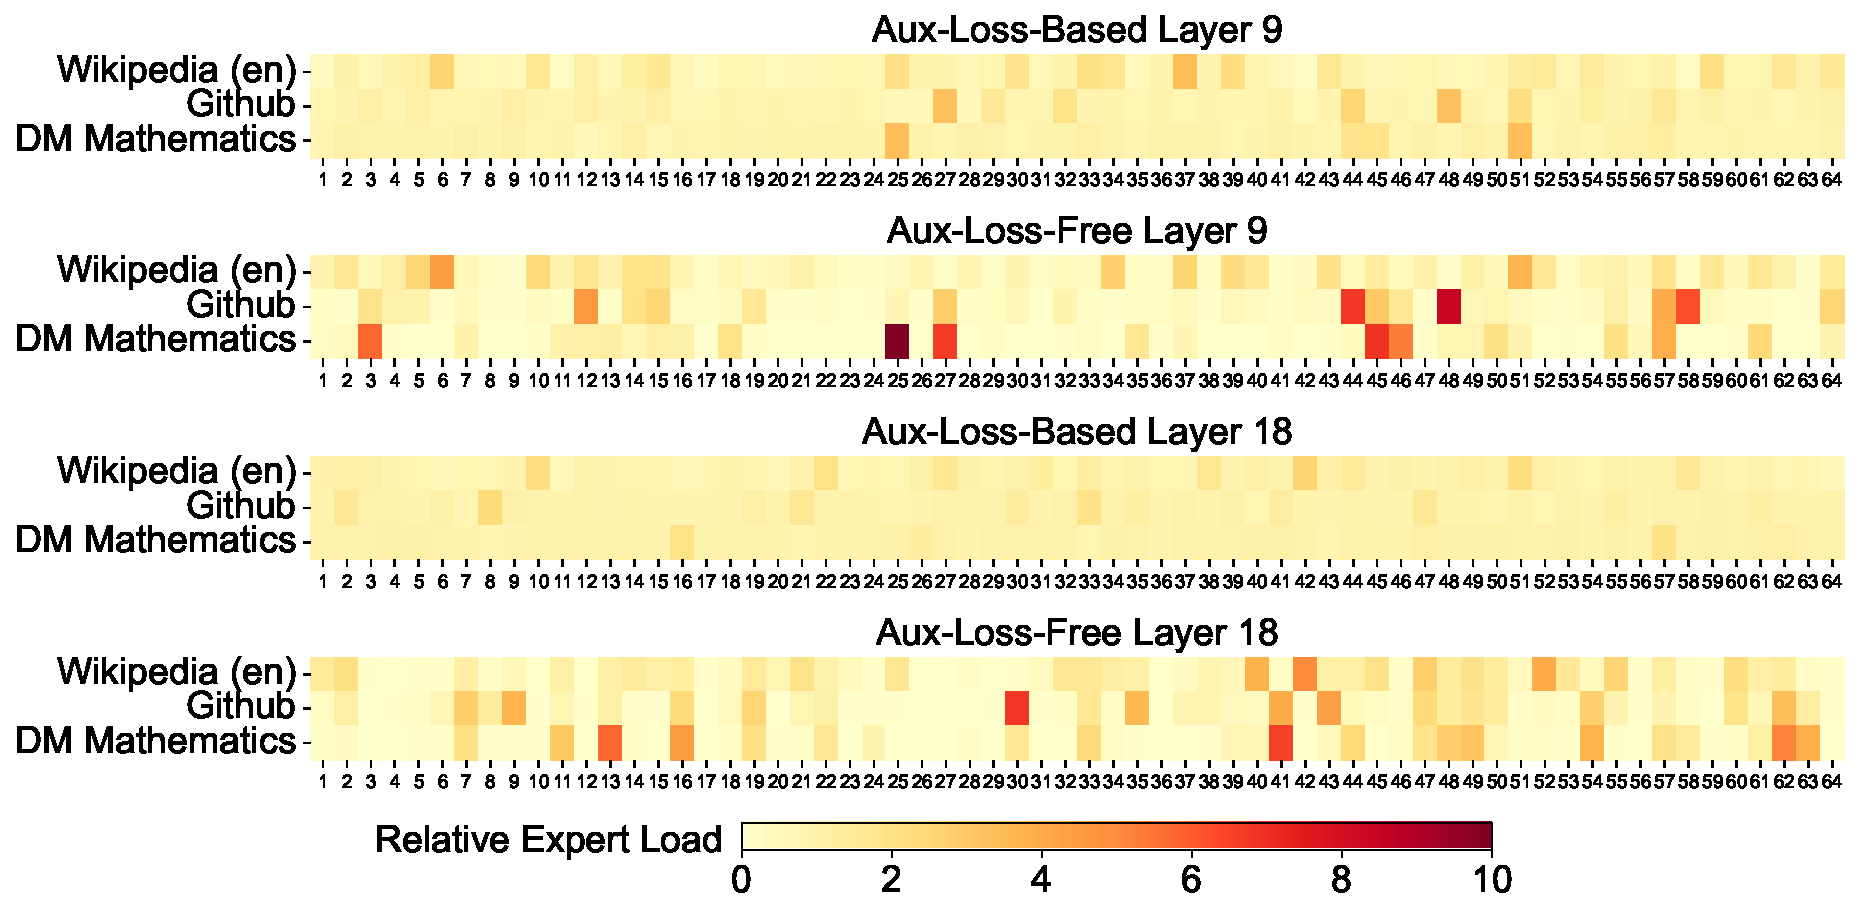
\includegraphics[width=0.99\linewidth]{figures/relative_expert_load_multi.pdf}
\caption{无辅助损失模型和基于辅助损失模型在 Pile 测试集三个领域的专家负载。无辅助损失模型表现出比基于辅助损失模型更明显的专家专业化模式。相对专家负载表示实际专家负载与理论平衡专家负载之间的比率。由于篇幅限制,我们仅展示两个层的结果作为示例,所有层的结果详见附录~\ref{app:detailed_expert_load}。}
\label{fig:expert_load}
\end{figure}

\section{后训练(Post-Training)}
\label{sec:alignment}

\subsection{监督微调(Supervised Fine-Tuning)}

我们精心策划了指令调优数据集,包括 150 万个实例,涵盖多个领域,每个领域采用不同的数据创建方法,以满足其特定需求。

\paragraph{推理数据。}
对于与推理相关的数据集,包括数学、代码竞赛问题和逻辑谜题,我们通过利用内部的 DeepSeek-R1 模型生成数据。具体来说,虽然 R1 生成的数据表现出较强的准确性,但也存在过度思考、格式不佳和长度过长等问题。我们的目标是平衡 R1 生成的推理数据的高准确性与常规格式化推理数据的清晰性和简洁性。

为了建立我们的方法论,我们首先开发一个专门针对特定领域(如代码、数学或一般推理)的专家模型,使用结合的监督微调(SFT)和强化学习(RL)训练流程。该专家模型作为最终模型的数据生成器。训练过程涉及为每个实例生成两种不同类型的 监督微调 样本:第一种将问题与其原始响应配对,格式为 <问题, 原始响应>;第二种则在问题和 R1 响应旁边添加系统提示,格式为 <系统提示, 问题, R1 响应>。

系统提示经过精心设计,包含指导模型生成丰富反思和验证机制的响应的指令。在 强化学习 阶段,模型利用高温采样生成响应,整合来自 R1 生成数据和原始数据的模式,即使在没有明确的系统提示的情况下。在经过数百步的 强化学习 训练后,中间 强化学习 模型学会了整合 R1 模式,从而战略性地提升整体性能。

完成 强化学习 训练阶段后,我们实现了拒绝采样,以策划高质量的 监督微调 数据供最终模型使用,专家模型被用作数据生成源。这种方法确保最终训练数据保留 DeepSeek-R1 的优点,同时生成简洁有效的响应。

\paragraph{非推理数据。}
对于非推理数据,如创意写作、角色扮演和简单问答,我们利用 DeepSeek-V2.5 生成响应,并招募人工注释员验证数据的准确性和正确性。

\paragraph{监督微调 设置。}
我们对 \dsviii{}-Base 进行两轮的微调,使用 监督微调 数据集,采用余弦衰减学习率调度,从 $5 \times 10^{-6}$ 开始,逐渐降低到 $1 \times 10^{-6}$。在训练过程中,每个单一序列由多个样本打包而成。然而,我们采用样本掩码策略,以确保这些示例保持隔离且相互不可见。

\subsection{强化学习}

\subsubsection{奖励模型}

我们在强化学习过程中采用基于规则的奖励模型(Rule-Based Reward Model,RM)和基于模型的奖励模型。

\paragraph{基于规则的奖励模型。}
对于可以通过特定规则验证的问题,我们采用基于规则的奖励系统来确定反馈。例如,某些数学问题具有确定的结果,我们要求模型以指定格式(例如,框内)提供最终答案,从而应用规则来验证正确性。同样,对于 LeetCode 问题,我们可以利用编译器根据测试用例生成反馈。通过尽可能利用基于规则的验证,我们确保了更高的可靠性,因为这种方法对操控或利用具有抵抗力。

\paragraph{基于模型的奖励模型。}
对于具有自由形式真实答案的问题,我们依赖奖励模型来判断响应是否与预期的真实答案匹配。相反,对于没有明确真实答案的问题,例如涉及创意写作的问题,奖励模型的任务是根据问题和相应答案作为输入提供反馈。奖励模型从 \dsviii{} 监督微调 检查点进行训练。为了增强其可靠性,我们构建了偏好数据,不仅提供最终奖励,还包括导致该奖励的思维链。这种方法有助于降低特定任务中奖励操控的风险。

\subsubsection{组相对策略优化(Group Relative Policy Optimization)}

与 \dsvii{} 类似,我们采用了组相对策略优化(GRPO),该方法放弃了通常与策略模型大小相同的评估模型,而是从组得分中估计基线。具体而言,对于每个问题 $q$,GRPO 从旧的策略模型 $\pi_{\theta_{old}}$ 中抽样一组输出 $\{o_1, o_2, \cdots, o_G\}$,然后通过最大化以下目标来优化策略模型 $\pi_{\theta}$:

\begin{equation}
\begin{split}
    \mathcal{J}_{GRPO}(\theta) &= \mathbb{E}{[q \sim P(Q), \{o_i\}_{i=1}^G \sim \pi_{\theta_{old}}(O|q)]}  \\
    & \frac{1}{G}\sum_{i=1}^G \left( \min \left( \frac{\pi_\theta(o_i |q)}{\pi_{\theta_{old}}(o_i |q)} A_i, \text{clip} \left( \frac{\pi_\theta(o_i |q)}{\pi_{\theta_{old}}(o_i |q)}, 1 - \epsilon, 1 + \epsilon \right)  A_i \right) - \beta \mathbb{D}_{KL}\left(\pi_{\theta} || \pi_{ref}\right)\right) ,
\end{split}
\label{eq:GRPO-obj}
\end{equation}

\begin{equation}
    \mathbb{D}_{KL}\left(\pi_{\theta} || \pi_{ref}\right) = \frac{\pi_{ref}(o_i|q)}{\pi_{\theta}(o_i|q)}- \log\frac{\pi_{ref}(o_i|q)}{\pi_{\theta}(o_i|q)} - 1,
\end{equation}

其中 $\epsilon$ 和 $\beta$ 是超参数;

$\pi_{ref}$ 是参考模型;

$A_i$ 是优势,来源于与每组内输出对应的奖励 ${r_1, r_2, \ldots, r_G}$:

\begin{equation}
    A_i = \frac{r_i - {\operatorname{mean}(\{r_1, r_2, \cdots, r_G\})}}{{\operatorname{std}(\{r_1, r_2, \cdots, r_G\})}}.
\end{equation}

我们在强化学习过程中融入了来自不同领域的提示,例如编程、数学、写作、角色扮演和问答。这种方法不仅使模型与人类偏好更加一致,还提高了基准测试中的表现,特别是在可用的 监督微调 数据有限的情况下。

\subsection{评估}

\subsubsection{评估设置}

\paragraph{评估基准。}
除了我们用于基础模型测试的基准外,我们还在 IFEval、FRAMES、LongBench v2、GPQA、SimpleQA、C-SimpleQA、SWE-Bench Verified、Aider~\footnote{\url{https://aider.chat}}、LiveCodeBench(2024年8月至2024年11月的问题)、Codeforces~\footnote{\url{https://codeforces.com}}、中国国家高中数学奥林匹克(CNMO 2024)\footnote{\url{https://www.cms.org.cn/Home/comp/comp/cid/12.html}}以及美国邀请数学考试 2024(AIME 2024)上进一步评估指令模型。

\paragraph{比较基线。}
我们对我们的聊天模型进行了全面评估,与多个强基线进行比较,包括 \dsvii{}-0506、DeepSeek-V2.5-0905、Qwen2.5 72B Instruct、LLaMA-3.1 405B Instruct、Claude-Sonnet-3.5-1022 和 GPT-4o-0513。对于 \dsvii{} 模型系列,我们选择最具代表性的变体进行比较。对于闭源模型,通过其各自的 API 进行评估。

\paragraph{详细评估配置。}
对于包括 MMLU、DROP、GPQA 和 SimpleQA 在内的标准基准,我们采用来自 simple-evals 框架的评估提示\footnote{\url{https://github.com/openai/simple-evals}}。我们在零-shot 设置中使用 Zero-Eval 提示格式进行 MMLU-Redux 的评估。对于其他数据集,我们遵循数据集创建者提供的原始评估协议和默认提示。对于代码和数学基准,HumanEval-Mul 数据集包括 8 种主流编程语言(Python、Java、C++、C\#、JavaScript、TypeScript、PHP 和 Bash)。我们使用 CoT 和非 CoT 方法评估模型在 LiveCodeBench 上的表现,数据收集时间为 2024 年 8 月至 2024 年 11 月。Codeforces 数据集的评估使用竞争者的百分比进行衡量。SWE-Bench Verified 使用无代理框架进行评估。我们使用“diff”格式评估与 Aider 相关的基准。对于数学评估,AIME 和 CNMO 2024 的评估温度为 0.7,结果在 16 次运行中取平均,而 MATH-500 则采用贪婪解码。我们允许所有模型在每个基准上输出最多 8192 个Token。

\begin{table}[h]
    \centering
    \footnotesize
    \setlength{\tabcolsep}{1.9pt}
    \begin{tabular}{@{}c l | c  c | c c c c| c@{}}
    \toprule
    & \multirow{2}{*}{\centering \textbf{Benchmark {\tiny (Metric)}}} & {\textbf{DeepSeek}} & {\textbf{DeepSeek}} & \textbf{Qwen2.5} & \textbf{LLaMA-3.1}  & \textbf{Claude-3.5-}  & \textbf{GPT-4o}& \textbf{DeepSeek} \\
    & & \textbf{V2-0506}& \textbf{V2.5-0905} & \textbf{72B-Inst.} & \textbf{405B-Inst.} & \textbf{Sonnet-1022}  & \textbf{0513} & \textbf{V3} \\
    \midrule
    & Architecture &  MoE & MoE & Dense & Dense &-&- & MoE \\
    & \# Activated Params & 21B & 21B & 72B & 405B& -&-& 37B \\
    & \# Total Params &  236B & 236B & 72B & 405B &-&-& 671B \\
    \midrule
    \multirow{8}{*}{English}&   MMLU {\tiny (EM)}  & 78.2 & 80.6 & 85.3& \textbf{88.6} & \textbf{88.3}&87.2 & \textbf{88.5} \\
     & MMLU-Redux {\tiny (EM)} &77.9 & 80.3 &  85.6 &86.2& \textbf{88.9}& 88.0 & \textbf{89.1}\\
    & MMLU-Pro {\tiny (EM)} & 58.5 &  66.2 & 71.6 &73.3 & \textbf{78.0} & 72.6 & 75.9\\
    & DROP {\tiny (3-shot F1)} &83.0 & 87.8 & 76.7 & 88.7 & 88.3 & 83.7 & \textbf{91.}\\
    & IF-Eval {\tiny (Prompt Strict)} &57.7 & 80.6 & 84.1 & 86.0 & \textbf{86.5} & 84.3 & 86.1\\
    & GPQA-Diamond {\tiny (Pass@1)} & 35.3 & 41.3& 49.0 & 51.1& \textbf{65.0} & 49.9 & 59.1\\
    & SimpleQA {\tiny (Correct)} & 9.0 & 10.2 & 9.1 & 17.1& 28.4 & \textbf{38.2}& 24.9\\
     & FRAMES {\tiny (Acc.)} & 66.9 & 65.4 & 69.8 & 70.0 & 72.5 & \textbf{80.5} & 73.3 \\
     & LongBench v2 {\tiny (Acc.)} & 31.6 & 35.4 & 39.4 & 36.1 & 41.0 & 48.1 &\textbf{48.7} \\
    \midrule
    \multirow{5}{*}{Code} & HumanEval-Mul {\tiny (Pass@1)} & 69.3 &77.4 & 77.3 & 77.2 & {81.7} &80.5&\textbf{82.6}\\
    & LiveCodeBench {\tiny (Pass@1-COT)} &18.8 & 29.2 & 31.1 & 28.4 & 36.3& 33.4& \textbf{40.5} \\
    & LiveCodeBench {\tiny (Pass@1)} &20.3 & 28.4 & 28.7 & 30.1 & 32.8& 34.2& \textbf{37.6} \\
    & Codeforces {\tiny (Percentile)} & 17.5 & 35.6 & 24.8 & 25.3 & 20.3 & 23.6 & \textbf{51.6} \\
    & SWE Verified {\tiny (Resolved)} &-&22.6& 23.8 & 24.5 & \textbf{50.8}&38.8&42.0\\
    & Aider-Edit {\tiny (Acc.)} & 60.3& 71.6 & 65.4 & 63.9 & \textbf{84.2} &72.9&79.7 \\
    & Aider-Polyglot {\tiny (Acc.)}  & -& 18.2 & 7.6 & 5.8 & 45.3&16.0&\textbf{49.6} \\
    \midrule
    \multirow{3}{*}{Math} & AIME 2024 {\tiny (Pass@1)} & 4.6 & 16.7 & 23.3 & 23.3 & 16.0 & 9.3 & \textbf{39.2} \\
    & MATH-500 {\tiny (EM)} &  56.3 & 74.7 & 80.0 & 73.8 & 78.3 & 74.6&\textbf{90.2} \\
    & CNMO 2024 {\tiny (Pass@1)} & 2.8 & 10.8 & 15.9& 6.8& 13.1 & 10.8 &\textbf{43.2} \\
    \midrule
    \multirow{3}{*}{Chinese} & CLUEWSC {\tiny (EM)} & 89.9& 90.4 & \textbf{91.4} & 84.7 & 85.4 & 87.9 & 90.9\\
    & C-Eval {\tiny (EM)} & 78.6& 79.5 & 86.1 & 61.5 & 76.7 & 76.0 & \textbf{86.5}\\
     & C-SimpleQA {\tiny (Correct)}  & 48.5& 54.1 & 48.4 & 50.4 & 51.3 & 59.3 & \textbf{64.8}\\
    \bottomrule
    \end{tabular}
    \caption{\dsviii{} 与其他代表性聊天模型的比较。所有模型在限制输出长度为 8K 的配置下进行评估。对于样本少于 1000 的基准测试,使用不同的温度设置进行多次测试,以得出稳健的最终结果。\dsviii{} 是表现最佳的开源模型,并且在与前沿的闭源模型相比时也展现了竞争力。}
    \label{tab:chat}
\end{table}

\subsubsection{标准评估}

表~\ref{tab:chat} 展示了评估结果,表明 \dsviii{} 是表现最好的开源模型。此外,它在与前沿闭源模型如 GPT-4o 和 Claude-3.5-Sonnet 的竞争中也表现出色。

\paragraph{英文基准测试}
MMLU 是一个广泛认可的基准,旨在评估大型语言模型在多种知识领域和任务中的表现。 \dsviii{} 展现出具有竞争力的性能,与顶尖模型如 LLaMA-3.1-405B、GPT-4o 和 Claude-Sonnet 3.5 不相上下,同时显著超越 Qwen2.5 72B。此外,\dsviii{} 在 MMLU-Pro 这一更具挑战性的教育知识基准测试中表现优异,接近 Claude-Sonnet 3.5。在 MMLU-Redux(一个修正标签的 MMLU 精简版)中,\dsviii{} 超越了其他同类模型。此外,在 GPQA-Diamond 这一博士级评估测试平台上,\dsviii{} 取得了卓越的成绩,仅次于 Claude 3.5 Sonnet,且显著超越了所有其他竞争对手。

在长文本理解基准测试中,如 DROP、LongBench v2 和 FRAMES,\dsviii{} 继续展示其作为顶尖模型的地位。在 DROP 的 3-shot 设置中,它取得了令人印象深刻的 91.6 F1 分数,超越了该类别中的所有其他模型。在 FRAMES 这一需要在超过 10 万个Token上下文中进行问答的基准测试中,\dsviii{} 紧随 GPT-4o,其表现显著优于其他所有模型。这展示了 \dsviii{} 在处理极长文本任务方面的强大能力。

\dsviii{} 的长文本处理能力在 LongBench v2 上得到了进一步验证,该数据集在 DeepSeek V3 发布前几周发布。在事实知识基准测试 SimpleQA 中,\dsviii{} 落后于 GPT-4o 和 Claude-Sonnet,这主要是由于其设计重点和资源分配。 \dsviii{} 将更多的训练Token分配给学习中文知识,从而在 C-SimpleQA 上表现出色。在遵循指令的基准测试中,\dsviii{} 显著超越了其前身 \dsvii{} 系列,突显了其在理解和遵循用户定义格式约束方面的改进能力。

\paragraph{代码与数学基准测试}
编程是大语言模型面临的一项具有挑战性且实用的任务,涵盖了工程相关的任务,如 SWE-Bench-Verified 和 Aider,以及算法任务,如 HumanEval 和 LiveCodeBench。在工程任务中,\dsviii{} 落后于 Claude-Sonnet-3.5-1022,但显著优于开源模型。开源的 \dsviii{} 有望促进与编码相关的工程任务的进展。通过提供其强大的能力,\dsviii{} 可以推动软件工程和算法开发等领域的创新与改进,使开发者和研究人员能够拓展开源模型在编程任务中的边界。

在算法任务中,\dsviii{} 展现出卓越的表现,超越了 HumanEval-Mul 和 LiveCodeBench 等基准测试中的所有基线。这一成功归因于其先进的知识蒸馏技术,有效提升了其在算法任务中的代码生成和问题解决能力。

在数学基准测试中,\dsviii{} 展现出卓越的表现,显著超越了基线,并为非 o1-like 模型设定了新的最先进水平。具体而言,在 AIME、MATH-500 和 CNMO 2024 上,\dsviii{} 的绝对得分比第二名模型 Qwen2.5 72B 高出约 10\%,这一差距在如此具有挑战性的基准测试中是相当显著的。这一卓越能力突显了 DeepSeek-R1 中蒸馏技术的有效性,该技术已被证明对非 o1-like 模型极为有益。

\paragraph{中文基准测试}
Qwen 和 DeepSeek 是两个在中文和英文方面具有强大支持的代表性模型系列。在事实基准测试中文 SimpleQA 中,\dsviii{} 超越了 Qwen2.5-72B 16.4 分,尽管 Qwen2.5 是在一个更大的语料库上训练的,包含 18T Token,比 \dsviii{} 预训练的 14.8T Token多出 20\%。

在 C-Eval(一个代表性的中文教育知识评估基准)和 CLUEWSC(中文 Winograd 语料库挑战)中,\dsviii{} 和 Qwen2.5-72B 表现出相似的性能水平,表明这两个模型在应对具有挑战性的中文推理和教育任务方面都经过了良好的优化。

\begin{table}[t]
    \centering
    \begin{tabular}{c | c c}
    \toprule
    \textbf{Model} & \textbf{Arena-Hard} & \textbf{AlpacaEval 2.0} \\
    \midrule
    DeepSeek-V2.5-0905 & 76.2 & 50.5\\
    Qwen2.5-72B-Instruct & 81.2 & 49.1  \\
    LLaMA-3.1 405B & 69.3 & 40.5\\
    GPT-4o-0513 & 80.4 &  51.1 \\
    Claude-Sonnet-3.5-1022 & 85.2  & 52.0 \\
    DeepSeek-V3 & \textbf{85.5} & \textbf{70.0} \\
    \bottomrule
    \end{tabular}
    \caption{英文开放性对话评估。对于 AlpacaEval 2.0,我们采用长度控制胜率作为评估标准。}
    \label{tab:open} 
\end{table}

\subsubsection{开放式评估}

除了标准基准测试,我们还使用大型语言模型(LLMs)作为评判者,对开放式生成任务进行了评估,结果如表~\ref{tab:open} 所示。具体而言,我们遵循了 AlpacaEval 2.0 和 Arena-Hard 的原始配置,利用 GPT-4-Turbo-1106 进行成对比较的评判。

在 Arena-Hard 上,\dsviii{} 以超过 86\% 的胜率击败基线模型 GPT-4-0314,其表现与顶尖模型如 Claude-Sonnet-3.5-1022 不相上下。这突显了 \dsviii{} 的强大能力,尤其是在处理复杂提示时,包括编码和调试任务。此外,\dsviii{} 成为第一个在 Arena-Hard 基准测试中超过 85\% 的开源模型,这一成就显著缩小了开源模型与闭源模型之间的性能差距,为开源模型在挑战性领域的成就设定了新标准。

同样,\dsviii{} 在 AlpacaEval 2.0 上表现出色,超越了闭源和开源模型。这证明了它在写作任务和处理简单问答场景方面的卓越能力。值得注意的是,它以 20\% 的显著优势超过了 DeepSeek-V2.5-0905,突显了在处理简单任务方面的重大改进,并展示了其进步的有效性。

\subsubsection{\dsviii{} 作为通用的奖励模型}

我们将 \dsviii{} 的判断能力与最先进的模型进行比较,即 GPT-4o 和 Claude-3.5。表~\ref{tab:rewardbench} 展示了这些模型在 RewardBench 中的表现。 

\dsviii{} 的表现与最佳版本的 GPT-4o-0806 和 Claude-3.5-Sonnet-1022 相当,同时超越了其他版本。此外,\dsviii{} 的判断能力还可以通过投票技术得到增强。因此,我们使用 \dsviii{} 结合投票技术,对开放式问题提供自我反馈,从而提高对齐过程的有效性和鲁棒性。

\begin{table}[t]
    \centering
    \begin{tabular}{c | c c c c c}
    \toprule
    \textbf{Model} & \textbf{Chat} & \textbf{Chat-Hard} & \textbf{Safety} & \textbf{Reasoning} & \textbf{Average} \\
    \midrule
    GPT-4o-0513 & 96.6 & 70.4 & 86.7 & 84.9 & 84.7\\
    GPT-4o-0806 & 96.1 & 76.1 & 88.1 & 86.6 & 86.7\\
    GPT-4o-1120 & 95.8 & 71.3 & 86.2 & 85.2 & 84.6\\
    \midrule 
    Claude-3.5-sonnet-0620 & 96.4 & 74.0 & 81.6 & 84.7 & 84.2\\
    Claude-3.5-sonnet-1022 & 96.4 & 79.7 & 91.1 & 87.6 & 88.7\\
    \midrule 
    \dsviii{} & 96.9 & 79.8 & 87.0 & 84.3 & 87.0\\
    \dsviii{} (maj@6) & 96.9 & 82.6 & 89.5 & 89.2 & 89.6\\
    \bottomrule
    \end{tabular}
    \caption{GPT-4o,Claude-3.5-sonnet 和 \dsviii{} 在 RewardBench 上的性能比较。}
    \label{tab:rewardbench}
\end{table}

\subsection{讨论}

\subsubsection{从 DeepSeek-R1 蒸馏}

我们基于 DeepSeek-V2.5 对来自 DeepSeek-R1 的蒸馏贡献进行了消融实验。基线模型是在短思维链(CoT)数据上训练的,而其竞争模型则使用了上述专家检查点生成的数据。

表~\ref{tab:distill} 显示了蒸馏数据的有效性,在 LiveCodeBench 和 MATH-500 基准测试中均显著提高了性能。我们的实验揭示了一个有趣的权衡:蒸馏导致了更好的性能,但也显著增加了平均响应长度。为了在模型准确性和计算效率之间保持平衡,我们为 \dsviii{} 在蒸馏中仔细选择了最佳设置。

我们的研究表明,从推理模型中进行知识蒸馏是后训练优化的一个有前景的方向。虽然我们目前的工作集中在数学和编程领域的数据蒸馏上,但这种方法在各种任务领域中显示出更广泛应用的潜力。在这些特定领域中展示的有效性表明,长思维链蒸馏可能对增强其他需要复杂推理的认知任务中的模型性能具有重要价值。进一步探索这种方法在不同领域的应用仍然是未来研究的重要方向。

\begin{table}[t]
    \centering
    \begin{tabular}{c|cc|cc}
    \toprule
    \multirow{2}{*}{\textbf{Model}} & \multicolumn{2}{c}{\textbf{LiveCodeBench-CoT}} & \multicolumn{2}{c}{\textbf{MATH-500}} \\

     & Pass@1 & Length & Pass@1 & Length\\
    \midrule
     DeepSeek-V2.5 Baseline & 31.1 & 718 & 74.6 & 769\\
     DeepSeek-V2.5 +R1 Distill & 37.4 & 783 &83.2& 1510\\
    \bottomrule
    \end{tabular}
    \caption{从 DeepSeek-R1 蒸馏的贡献。LiveCodeBench 和 MATH-500 的评估设定和表~\ref{tab:chat}中的一致。}
    \label{tab:distill} 
\end{table}

\subsubsection{自我奖励(Self-Rewarding)}

奖励在强化学习中发挥着关键作用,引导优化过程。在一些通过外部工具验证相对简单的领域,例如某些编程或数学场景,强化学习表现出卓越的效果。然而,在更一般的场景中,通过硬编码构建反馈机制是不可行的。在 \dsviii{} 的开发过程中,对于这些更广泛的背景,我们采用了宪法 AI (Constitutional AI)方法,利用 \dsviii{} 自身的投票评估结果作为反馈来源。这种方法产生了显著的对齐效果,显著提升了 \dsviii{} 在主观评估中的表现。通过整合额外的宪法输入,\dsviii{} 可以朝着宪法方向进行优化。

我们相信,这种将补充信息与大语言模型结合作为反馈来源的范式至关重要。大语言模型作为一个多功能处理器,能够将来自不同场景的非结构化信息转化为奖励,最终促进大语言模型的自我改进。除了自我奖励外,我们还致力于发现其他通用且可扩展的奖励方法,以持续提升模型在一般场景中的能力。

\subsubsection{多Token预测评估}

\dsviii{} 不仅仅预测下一个单个Token,而是通过 MTP 技术预测下两个Token。结合推测解码的框架,可以显著加快模型的解码速度。

一个自然的问题是关于额外预测Token的接受率。根据我们的评估,第二个Token预测的接受率在不同生成主题中范围在 85\% 到 90\% 之间,显示出一致的可靠性。这个高接受率使得 \dsviii{} 能够实现显著提高的解码速度,达到 1.8 倍的 TPS(每秒Token数)。

\section{结论,局限性和未来的方向}
\label{sec:conclusion}

在本文中,我们介绍了 \dsviii{},这是一个大型 MoE 语言模型,具有 671B 的总参数和 37B 的激活参数,训练数据量达到 14.8T Token。除了 \dsattn{} 和 \dsmoe{} 架构外,它还开创了一种无辅助损失的负载均衡策略,并设定了多Token预测训练目标,以实现更强的性能。

由于支持 FP8 训练和精细的工程优化,\dsviii{} 的训练具有成本效益。后训练阶段成功地从 DeepSeek-R1 系列模型中提炼了推理能力。全面评估表明,DeepSeek-V3 已成为当前最强的开源模型,并且在性能上与领先的闭源模型如 GPT-4o 和 Claude-3.5-Sonnet 相媲美。

尽管性能强大,但它仍保持了经济的训练成本。完整训练(包括预训练、上下文长度扩展和后训练)仅需 2.788M H800 GPU 小时。

尽管我们认可\dsviii{}的强大性能和成本效益,但我们也认识到它存在一些局限性,尤其是在部署方面。首先,为了确保高效的推理,\dsviii{}的推荐部署单元相对较大,这可能会对小型团队造成负担。其次,尽管我们对\dsviii{}的部署策略已经实现了端到端生成速度比\dsvii{}快两倍以上,但仍存在进一步优化的潜力。幸运的是,随着更先进硬件的发展,这些局限性有望自然得到解决。

DeepSeek 始终坚持开放源代码模型的长期发展路线,旨在稳步接近 AGI(人工通用智能)的最终目标。未来,我们计划在以下方向进行战略性投资研究。

\begin{itemize}
    \item 
    我们将持续研究和优化我们的模型架构,旨在进一步提高训练和推理效率,努力实现对无限上下文长度的高效支持。此外,我们还将尝试突破 Transformer 的架构限制,从而推动其建模能力的边界。
    \item 
    我们将不断迭代训练数据的数量和质量,并探索纳入额外训练信号来源,旨在推动数据在更广泛维度上的扩展。
    \item 
    我们将持续探索和迭代模型的深度思考能力,旨在通过扩展推理的长度和深度来增强模型的智能和解决问题的能力。
    \item 
    我们将探索更全面和多维度的模型评估方法,以防止在研究中倾向于优化固定的一组基准,这可能会对模型能力产生误导性的印象,并影响我们的基础评估。
\end{itemize}

\newpage
\appendix

\section*{Appendix}

\section{低精度训练的融合研究}
\label{app:fp8}

\begin{figure}[!h]
\centering
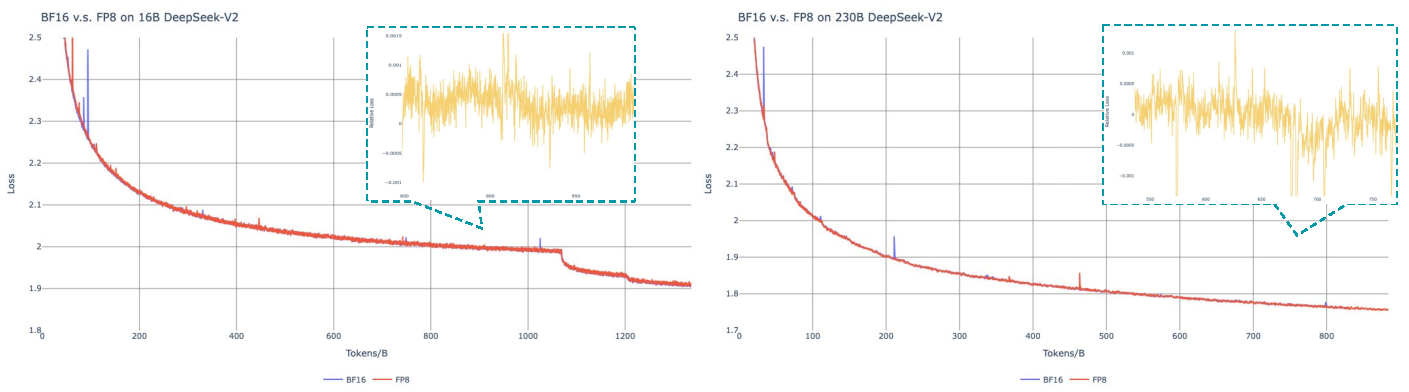
\includegraphics[width=0.95\linewidth]{figures/fp8-v.s.-bf16-repaired.pdf}
\caption{BF16 和 FP8 训练的损失曲线比较。结果通过指数移动平均(EMA)平滑,系数为 0.9。}
\label{fig:fp8_vs_bf16}
\end{figure}

\subsection{FP8训练 v.s. BF16训练}
\label{app:fp8_cp_bf16}

我们通过与两种基线模型在不同规模上进行比较,验证了我们的 FP8 混合精度框架与 BF16 训练的效果。在小规模上,我们训练了一个基线 MoE 模型,总参数约为 16B,使用了 1.33T 的Token。在大规模上,我们训练了一个基线 MoE 模型,总参数约为 230B,使用了大约 0.9T 的Token。我们在图~\ref{fig:fp8_vs_bf16} 中展示了训练曲线,并证明在我们的高精度累积和细粒度量化策略下,相对误差保持在 0.25\% 以下。

\subsection{有关块级量化的讨论}
\label{app:fp8_blockwise}

尽管我们的块状细粒度量化有效减轻了特征异常值引入的误差,但它需要对激活量化进行不同的分组,即在前向传播中使用 \texttt{1x128},而在反向传播中使用 \texttt{128x1}。激活梯度也需要类似的过程。一种简单的策略是对每 \texttt{128x128} 元素进行块状量化,就像我们对模型权重进行量化的方式一样。这样,反向传播时只需要进行转置。因此,我们进行了一项实验,其中与 \texttt{Dgrad} 相关的所有张量都在块状基础上进行量化。结果显示,计算激活梯度并以链式方式向浅层反向传播的 \texttt{Dgrad} 操作对精度非常敏感。具体而言,对激活梯度进行块状量化会导致一个约 16B 总参数的 MoE 模型在训练约 300B Token时发生模型发散。我们假设这种敏感性产生的原因是激活梯度在Token之间高度不平衡,导致与Token相关的异常值。这些异常值无法通过块状量化方法有效管理。

\section{16B 辅助损失模型和无辅助损失模型的专家专长模式}
\label{app:detailed_expert_load}

我们记录了 16B 辅助损失基线模型和无辅助损失模型在 Pile 测试集上的专家负载。无辅助损失模型在所有层次上通常具有更强的专家专长,如图~\ref{fig:detailed_expert_load} 所示。

\begin{figure}[!t]
    \subfigure[Layers 1-7]{
        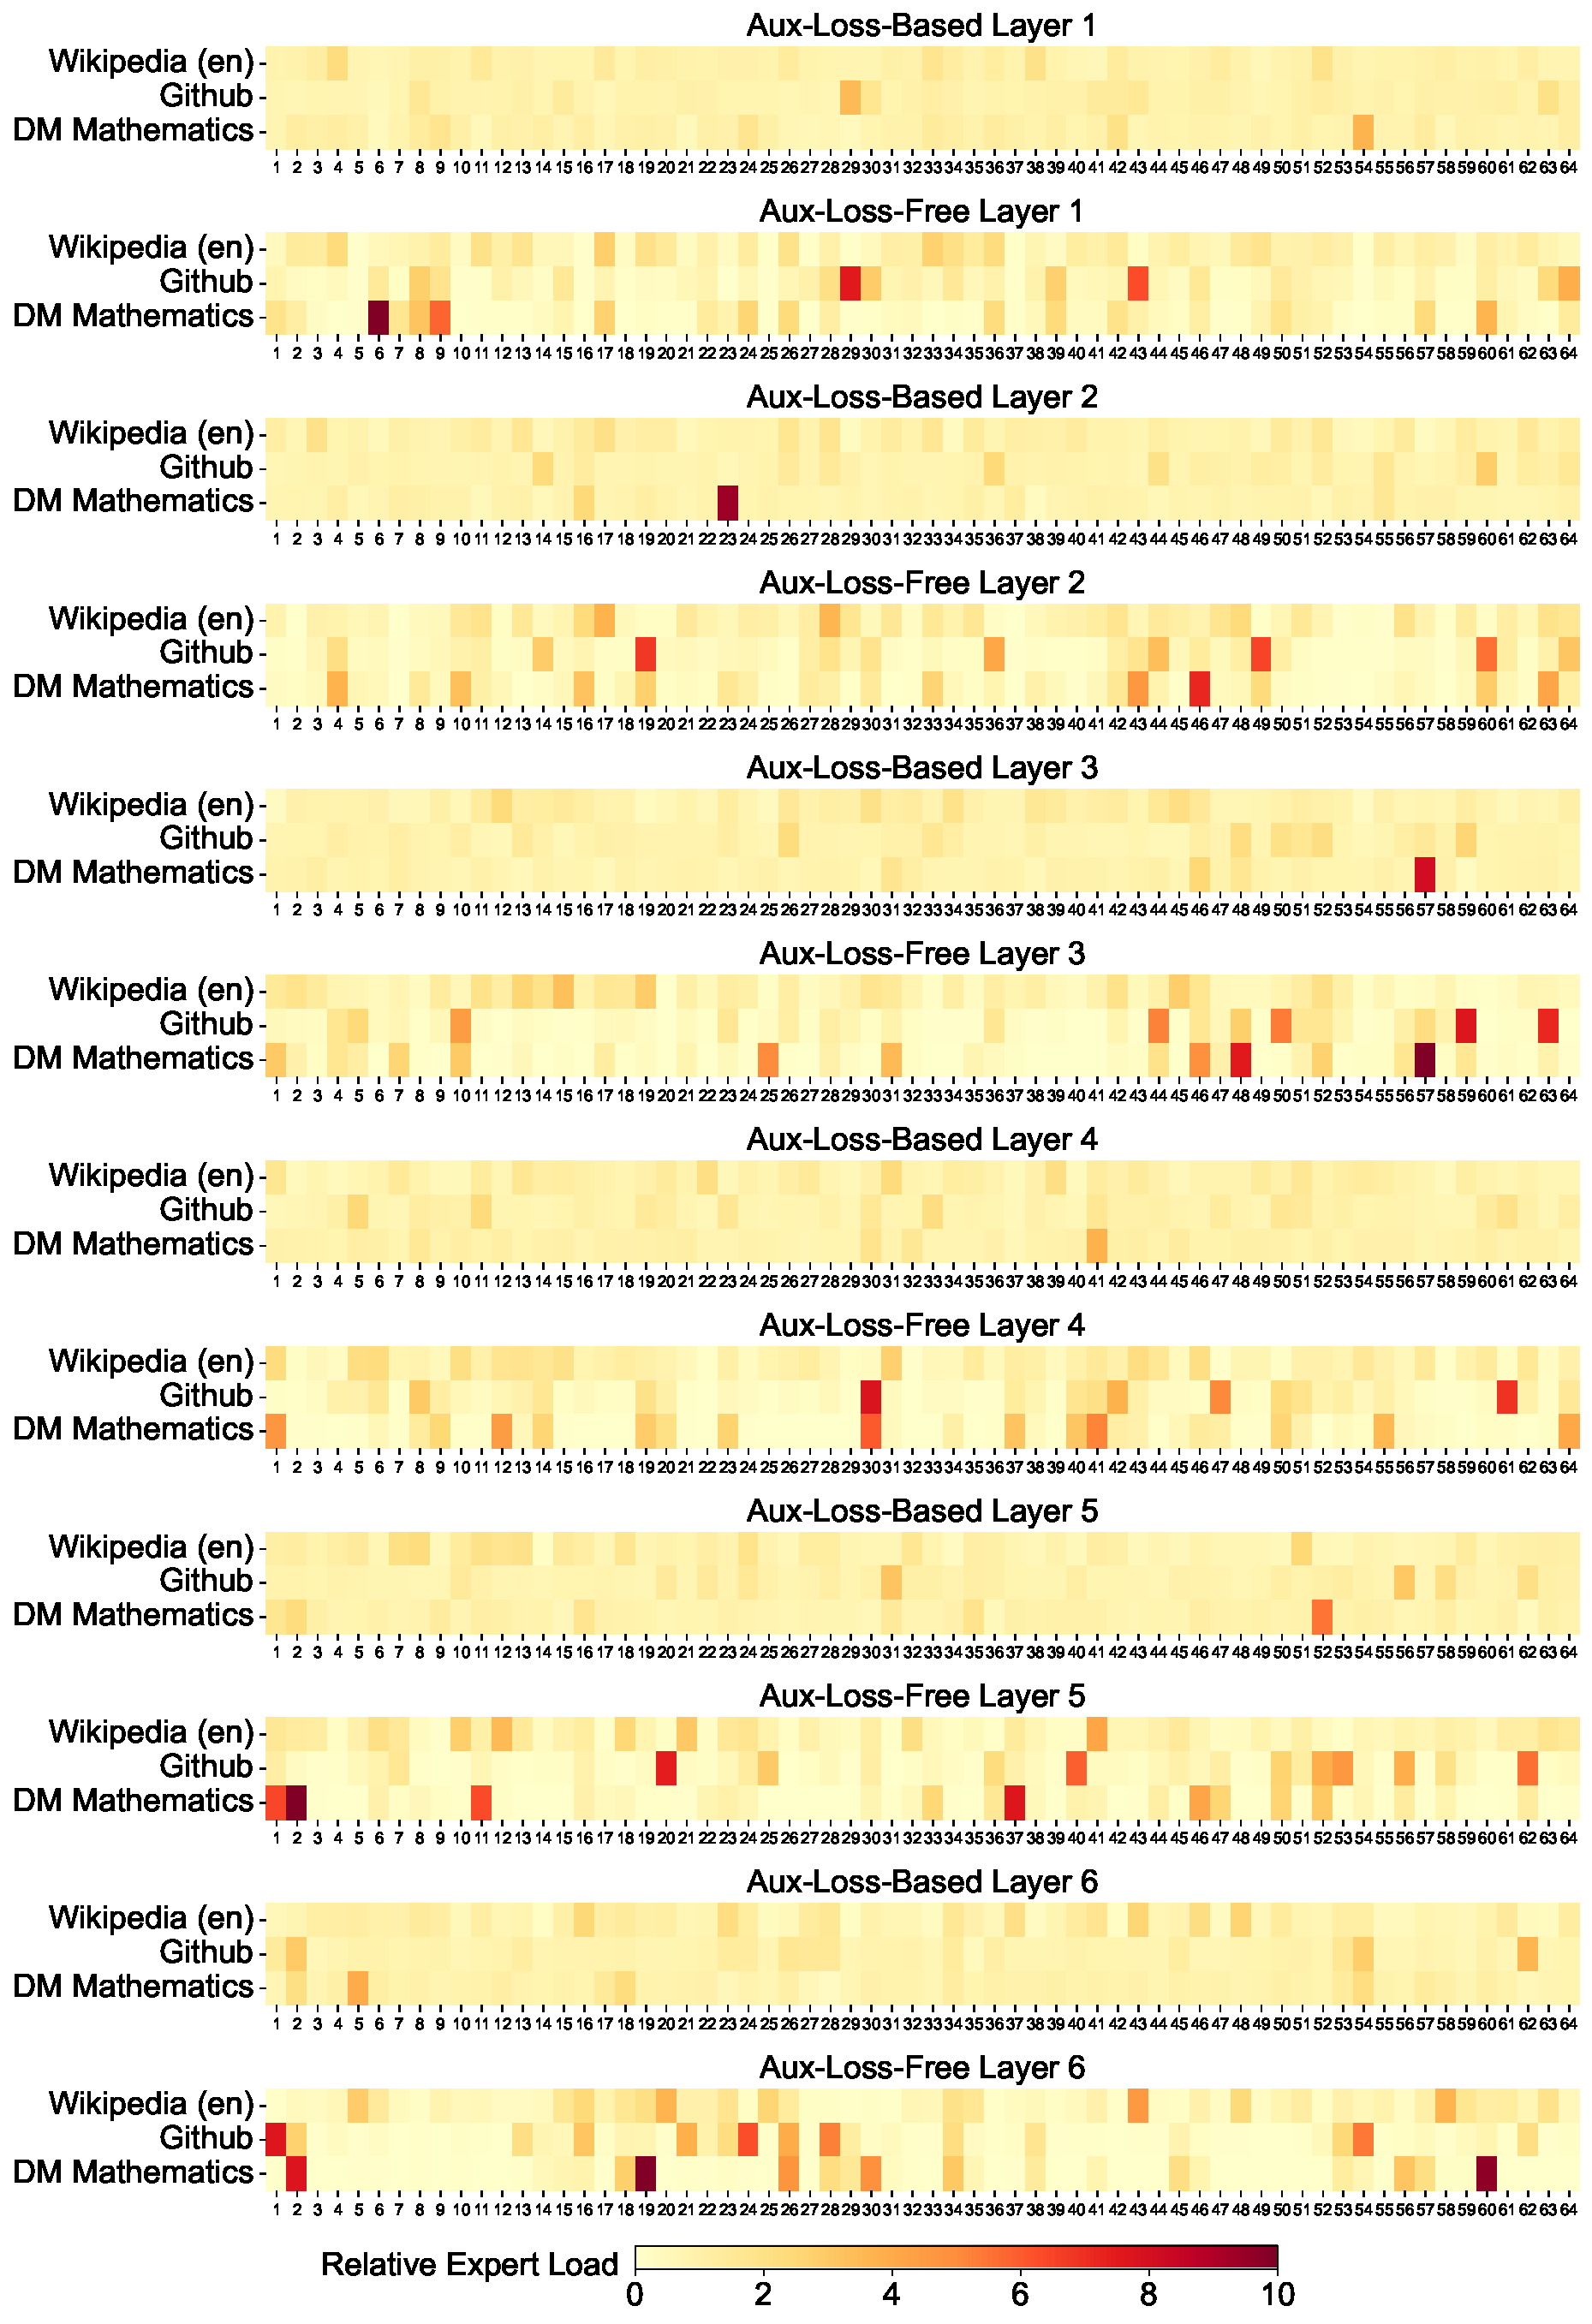
\includegraphics[width=0.95\linewidth]{figures/relative_expert_load_multi_1-6.pdf}
    }
\end{figure}

\begin{figure}[!t]
    \ContinuedFloat
    \subfigure[Layers 7-13]{
        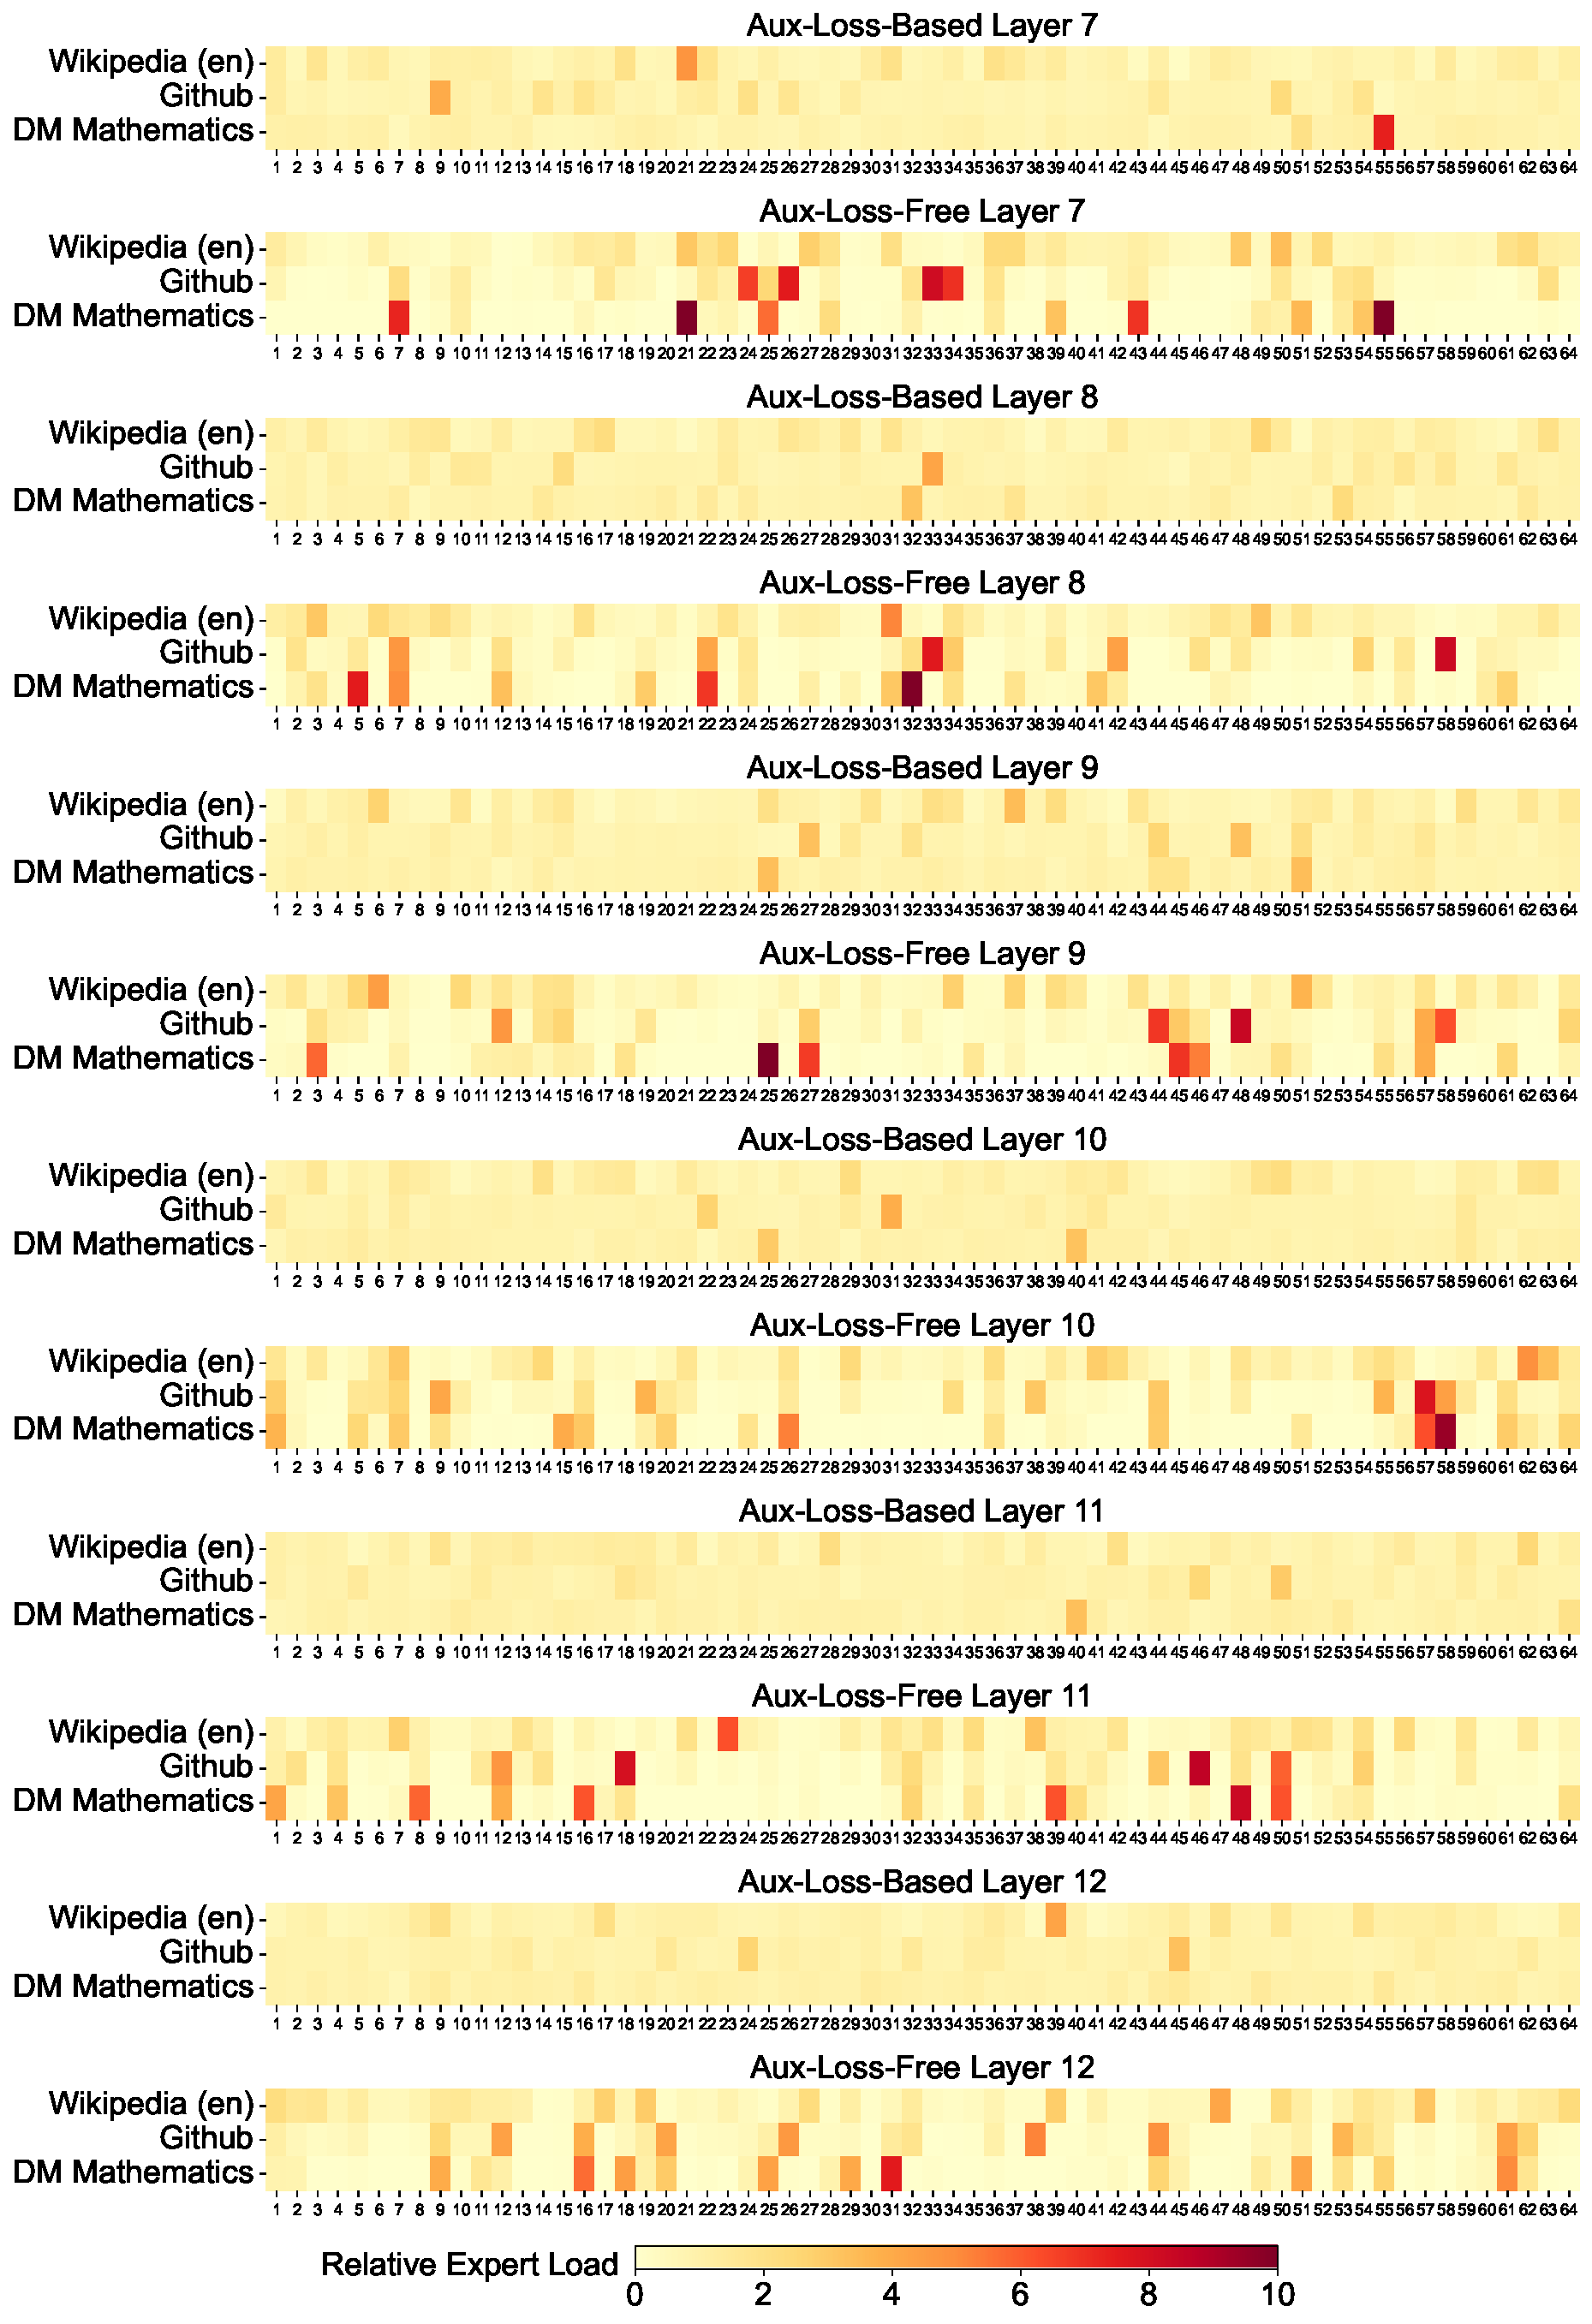
\includegraphics[width=0.95\linewidth]{figures/relative_expert_load_multi_7-12.pdf}
    }
\end{figure}

\begin{figure}[!t]
    \ContinuedFloat
    \subfigure[Layers 13-19]{
        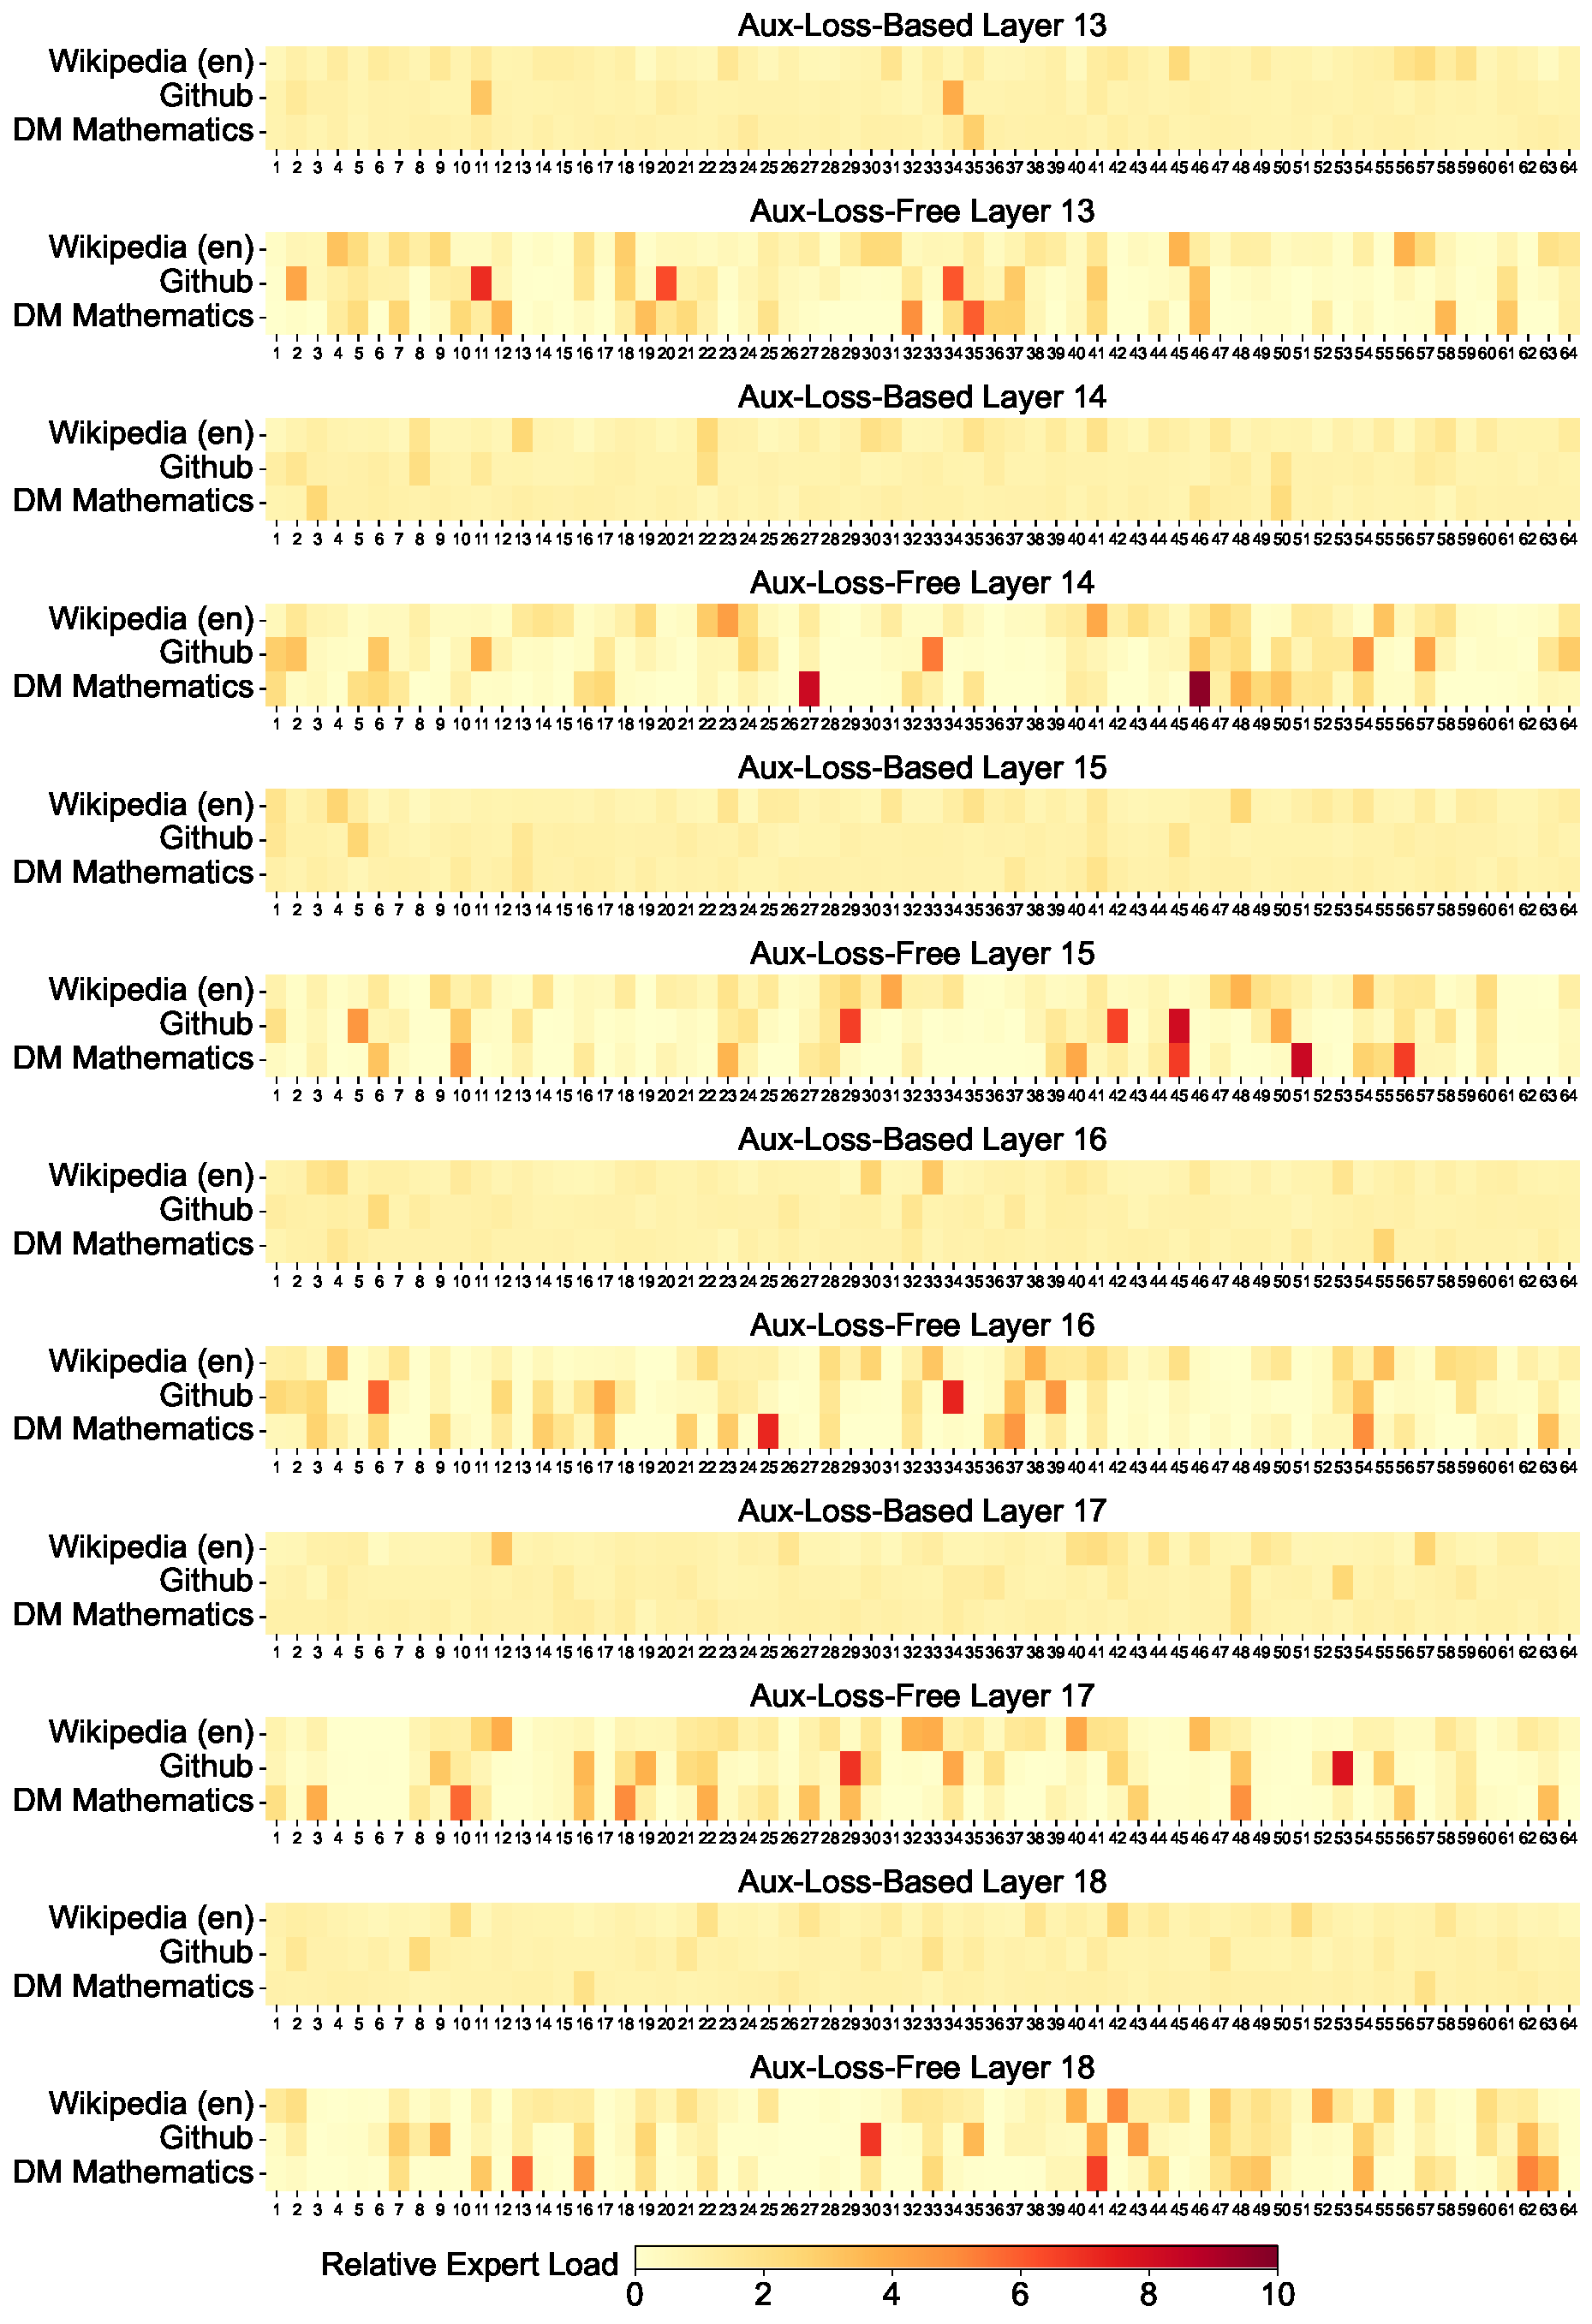
\includegraphics[width=0.95\linewidth]{figures/relative_expert_load_multi_13-18.pdf}
    }
\end{figure}

\begin{figure}[!t]
    \ContinuedFloat
    \subfigure[Layers 19-25]{
        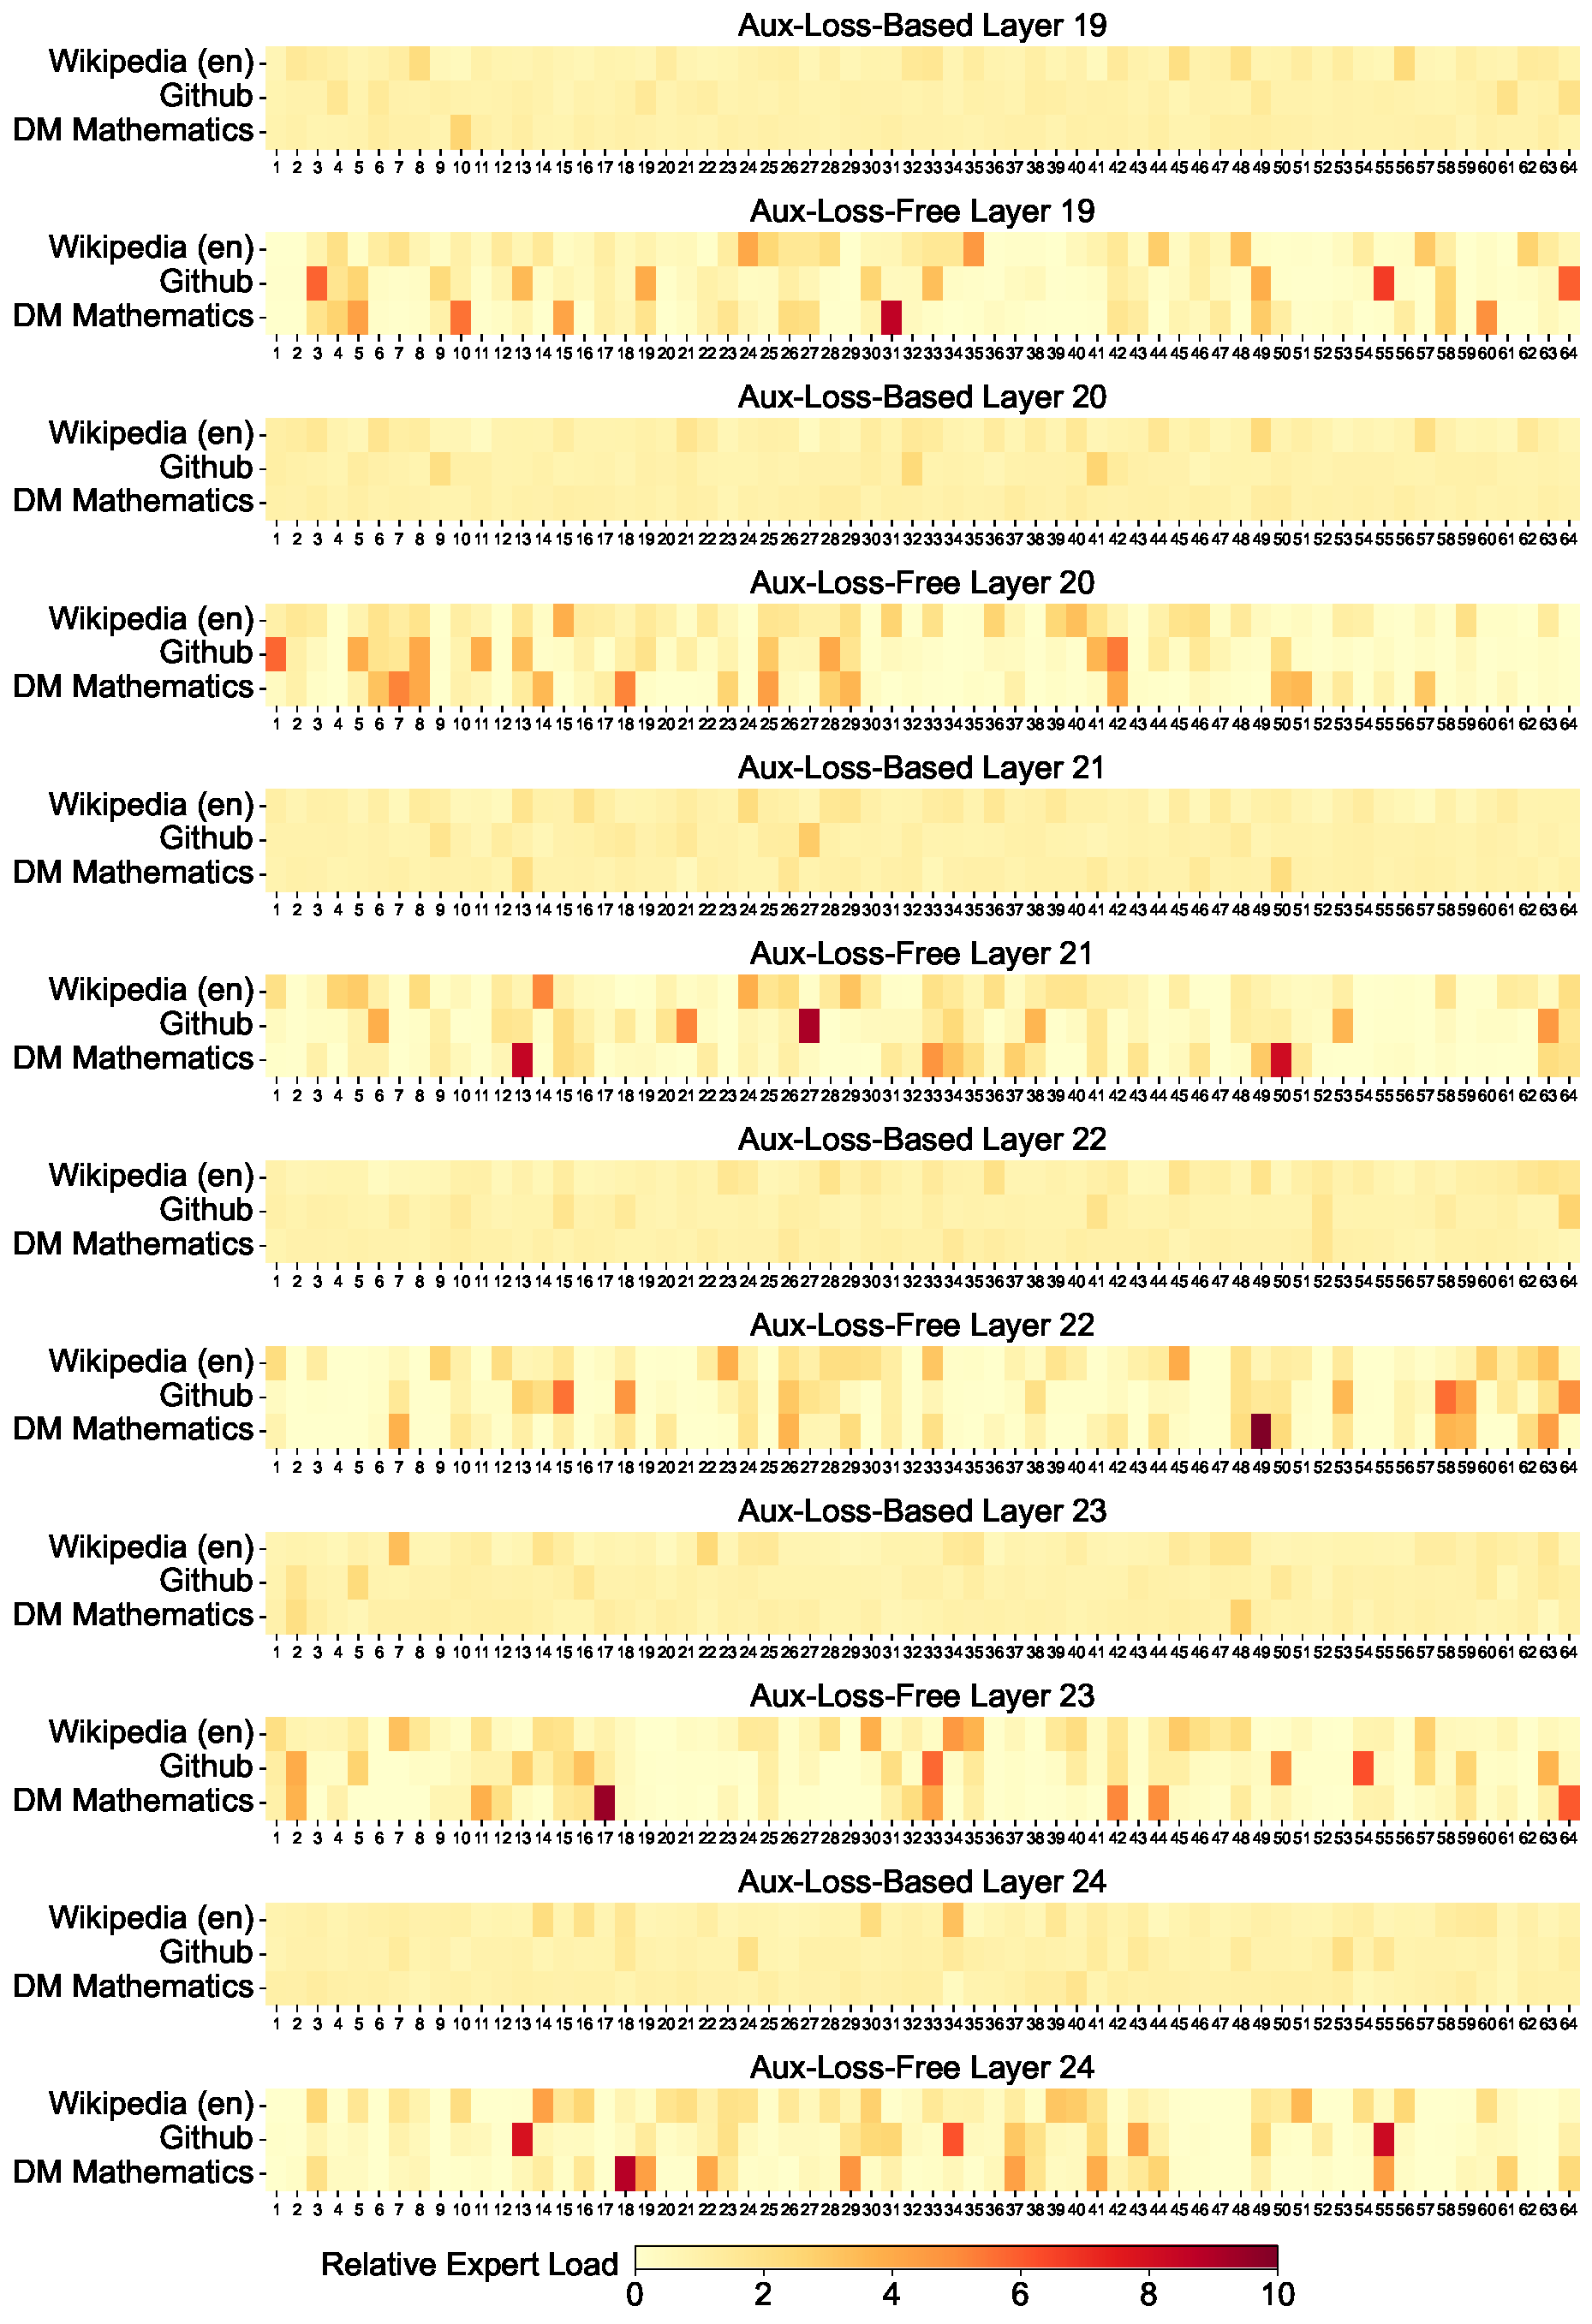
\includegraphics[width=0.95\linewidth]{figures/relative_expert_load_multi_19-24.pdf}
    }
\end{figure}

\begin{figure}[!t]
    \ContinuedFloat
    \subfigure[Layers 25-27]{
        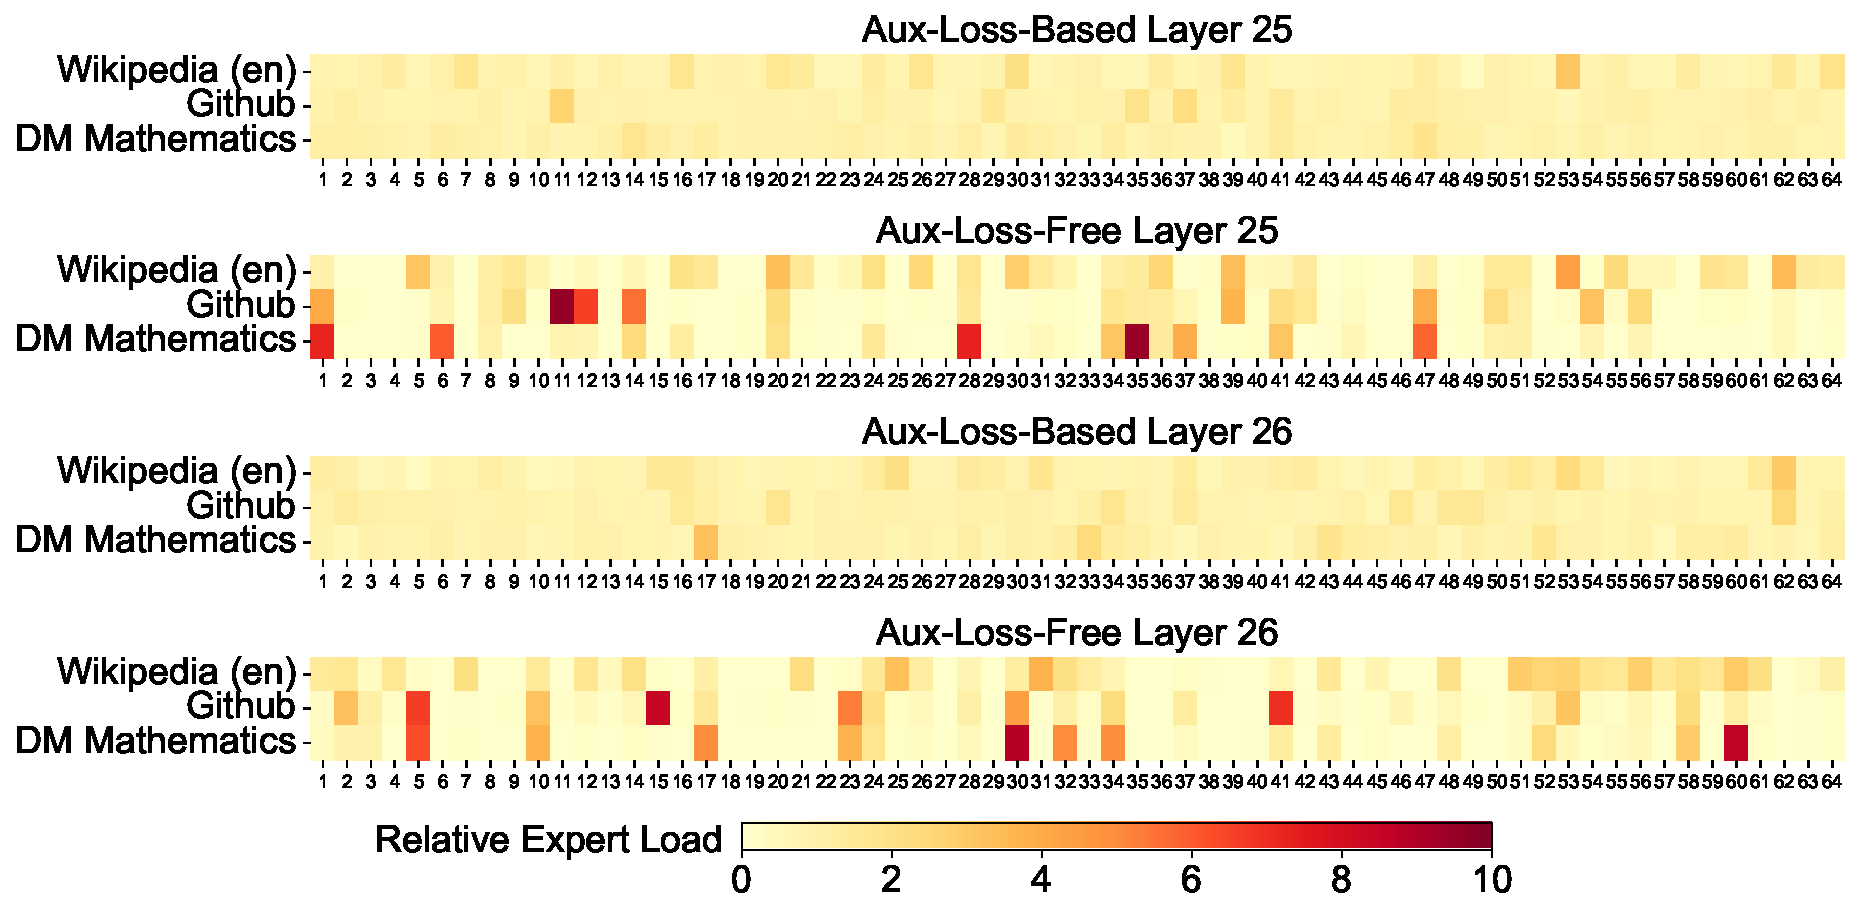
\includegraphics[width=0.95\linewidth]{figures/relative_expert_load_multi_25-26.pdf}
    }
    \caption{无辅助损失模型和有辅助损失模型在 Pile 测试集三个领域的专家负载。无辅助损失模型显示出比有辅助损失模型更强的专家专长模式。相对专家负载表示实际专家负载与理论平衡专家负载之间的比率。}
\label{fig:detailed_expert_load}
\end{figure}

\newpage

\end{document}
